%% JAIR submission format: the official jair.cls (JAIR Author Kit,
%% 2025/08/15) extending acmart, with BibLaTeX/biber and the acmauthoryear
%% style as the kit's template mandates. Build: pdflatex -> biber ->
%% pdflatex x2 (latexmk handles the cycle).
\documentclass[manuscript, screen, review]{jair}

\setcopyright{cc}
\acmDOI{10.1613/jair.1.xxxxx}

\JAIRAE{}
\JAIRTrack{}
\acmVolume{1}
\acmArticle{1}
\acmMonth{8}
\acmYear{2026}

%% The acmauthoryear citation style defines \citep and \citet itself
%% (acmauthoryear.cbx), so biblatex's natbib compatibility module must NOT
%% also be loaded: with natbib=true both define the same commands and the
%% second definition errors. The manuscript uses only \citep and \citet.
\RequirePackage[
  datamodel=acmdatamodel,
  style=acmauthoryear,
  backend=biber,
  giveninits=true,
  uniquename=init
  ]{biblatex}

\renewcommand*{\bibopenbracket}{(}
\renewcommand*{\bibclosebracket}{)}

\addbibresource{full_paper_jair.bib}

\usepackage{nicefrac}
\usepackage{multirow}
\usepackage{enumitem}
\graphicspath{{./}{../}}

%% acmart creates the theorem counter inside \AtEndPreamble, so a bare
%% \newtheorem here would run before the counter exists and error. Deferring
%% to \AtBeginDocument runs after every end-preamble hook.
\AtBeginDocument{\newtheorem{remark}[theorem]{Remark}}

\begin{document}

\title{Pricing the Sensing Budget in $\rho$-POMDPs,\\
with Expected Free Energy as the Canonical Information Weight}

\author{Patrick Cooper}
\affiliation{%
  \institution{Department of Computer Science, University of Colorado Boulder}
  \city{Boulder}
  \state{CO}
  \country{USA}
}
\email{patrick.cooper@colorado.edu}

\author{Alvaro Velasquez}
\affiliation{%
  \institution{Department of Computer Science, University of Colorado Boulder}
  \city{Boulder}
  \state{CO}
  \country{USA}
}
\email{alvaro.velasquez@colorado.edu}

\renewcommand{\shortauthors}{Cooper and Velasquez}

\begin{abstract}
\textbf{Background:} An agent acting under partial observability must decide how much effort to spend gathering information before committing to a decision. Standard POMDPs give it no direct way to state that spending limit, because information has value only through its downstream effect on reward. The $\rho$-POMDP framework rewards uncertainty reduction directly through a belief-dependent utility, but the weight placed on that utility is normally tuned by hand per task.
\textbf{Objectives:} We aim to (1) replace that hand-tuned weight with the operational shadow price of an explicitly stated sensing budget, so the design question becomes how much sensing can be afforded rather than what number the information term should carry, and (2) establish that active inference's Expected Free Energy supplies a principled anchor point on the resulting price curve rather than a searched hyperparameter.
\textbf{Methods:} We reformulate the information weight as the operational shadow price $w^*(B)$ of a sensing budget $B$, the weight at which the agent's induced sensing usage meets $B$. We prove exact scale equivariance for the implemented receding-horizon agent and monotone comparative statics for exact maximizers, define a set-valued price at usage gaps, and give an online dual controller with a stationary convergence guarantee and empirically demonstrated re-adaptation under reward-scale shift. We then prove that minimizing Expected Free Energy is exactly equivalent to solving a $\rho$-POMDP whose utility is expected information gain at weight $w{=}1$, for observe-then-commit POMDPs and, for the hidden-state-preserving observation and navigation actions, factored observation POMDPs covering the interleaved observe-act problems we study. The identification is exact under log scoring rules \citep{bernardo1979}. We evaluate both results against same-horizon planning, tuned information gain, POMCP on four of the observe-then-commit environments and on RockSample, and a near-optimal SARSOP reference on the three core observe-then-commit environments, across a suite spanning the classic Tiger problem, five further observe-then-commit environments, a cost-modified RockSample variant, and a Structural Inspection benchmark with over $65{,}000$ states.
\textbf{Results:} The budgeted formulation is exactly scale equivariant for the implemented agent, its usage curves collapse across reward scales, its closed-form onset thresholds are recovered as the first knot of the usage staircase, and the online dual controller tracks a stated budget through a tenfold reward rescale. The canonical untuned weight $w{=}1$ lands inside the reward-maximizing weight bracket on three of five swept environments and is beaten on the two exceptions, Testbed, where the reward-tied bracket sits at the low-weight boundary, and Tileworld, where the surface has a genuinely interior optimum. It remains competitive with per-task tuned information bonuses and is statistically equivalent to a near-optimal SARSOP reference, by TOST at the predeclared sensing-cost margin, on the three core observe-then-commit environments.
\textbf{Conclusions:} An information-gain utility's weight is best understood, and used, as the shadow price of an explicit sensing budget. Expected Free Energy supplies one canonical point on that price curve, an information-unit weight derived relative to the reward convention rather than searched per task. The design question changes from what the information weight should be to how much sensing the problem can afford.
\end{abstract}

%% JAIR note: do not include ACM CCS Concepts or keywords.

\maketitle

\section{Introduction}

Decision-making under partial observability requires agents to balance exploiting current knowledge against gathering information to reduce uncertainty about hidden states. In standard POMDPs, information gathering has no intrinsic value. It is useful only insofar as it leads to higher expected reward. This creates a well-known difficulty. The exploration--exploitation trade-off must be resolved either by the planning horizon or by heuristic exploration bonuses.

The $\rho$-POMDP framework \citep{araya2010} addresses this by extending POMDPs with a belief-dependent utility $\rho(b)$ that allows the agent to derive value directly from properties of its belief state. This enables explicit optimization over uncertainty reduction, information gain, or other belief-state properties alongside task reward. However, the choice of $\rho$ remains largely heuristic and environment-specific, and, when $\rho$ is an information-gain term, so does the weight placed on it.

This paper treats that weight as a design problem with a resource-allocation answer. State a sensing budget $B$, the amount of observation the agent may use before committing, and price the information-gain utility at the budget's \emph{operational shadow price} $w^*(B)$, which is the weight at which the agent chooses to spend about $B$ on sensing. That price is computable offline from a usage curve relating weight to expected sensing usage (Section~\ref{sec:budget}), trackable online by dual descent, with stationary convergence guaranteed (Proposition~\ref{prop:pi5}) and re-adaptation under mid-run reward-scale shift demonstrated empirically (Section~\ref{sec:dual_multiseed}). It is exactly scale equivariant for the implemented agent, so it need not be re-tuned when rewards are rescaled (Proposition~\ref{prop:pi1}). And it is set-valued, a bracket rather than a point, whenever the budget falls at a usage gap (Definition~\ref{def:pi3}). The question ``what weight should the information-gain utility carry'' becomes ``how much sensing can we afford,'' with the weight read off the stated budget rather than searched per task.

The active inference (AIF) framework \citep{friston2010, parr2019} identifies one canonical point on this price curve. AIF casts perception and action as approximate Bayesian inference, selecting policies that minimize Expected Free Energy (EFE). EFE naturally decomposes into a pragmatic term (goal-seeking) and an epistemic term (information-seeking). Because both terms come from a single variational objective, their relative coefficient is fixed once pragmatic value is identified with task reward. In the discrete-state formulation we use, that coefficient is $w{=}1$ in information units (Proposition~\ref{prop:equivalence}). The claim is exact under log scoring rules \citep{bernardo1979} and, under a shared reward convention, an empirically robust untuned default. It is not scale-invariant. Multiplying every reward and cost by $\alpha>0$ leaves the bit-valued information term unchanged, so a fixed $w{=}1$ implements a different trade-off at every scale. Rather than treating this as a limitation to caveat, we read it as confirmation that $w$ is a price. $w{=}1$ is recovered as exactly the special case of the budgeted formulation above that buys whatever sensing the ambient reward scale happens to imply, not a universal, scale-invariant calibration. A convention-free comparison between a reward-denominated quantity and a bit-denominated one is not on offer to any fixed weight, ours included. What the log-scoring derivation supplies is a principled anchor within that unavoidable choice rather than an escape from it, which is the sense in which $w{=}1$ remains an untuned default even though it is not a scale-invariant one.

We treat the information weight as a price and Expected Free Energy as one canonical point on the price curve, yielding an agent whose epistemic foraging is a consequence of a stated budget rather than an engineered bonus.\footnote{Code and experiment data are available at \url{https://github.com/PatrickAllenCooper/rho_aif}.} Our contributions are:
\begin{enumerate}
    \item Budgeted reformulation. We recast the information weight as the operational shadow price $w^*(B)$ of a sensing budget $B$ (Section~\ref{sec:budget}), prove exact scale equivariance of the resulting policy family for the implemented receding-horizon agent (Proposition~\ref{prop:pi1}), define a set-valued price at usage gaps (Definition~\ref{def:pi3}), and give an online dual controller with a stationary convergence guarantee (Proposition~\ref{prop:pi5}) whose decaying-step controller, with and without a reset-on-shift clock, re-adapts empirically under reward-scale shift (Section~\ref{sec:dual_multiseed}). This is the paper's primary contribution. It turns a hyperparameter into a stated resource constraint.
    \item Theory. A formal bridge between $\rho$-POMDPs and active inference, which is what licenses reading $w{=}1$ as an anchor on the price curve rather than an arbitrary choice. We prove the equivalence for observe-then-commit POMDPs (Proposition~\ref{prop:equivalence}), characterize when the information-unit weight $w{=}1$ is near-optimal (Proposition~\ref{prop:nearopt}), and extend the equivalence to factored observation POMDPs, interleaved settings where information gathering preserves the hidden state (Proposition~\ref{prop:factored}).
    \item Evidence. Controlled comparisons against same-horizon planning and tuned information gain across six observe-then-commit environments (Tiger, Diagnosis, Bandit, Tileworld, the two-state Testbed, and the distractor variant of Diagnosis, with the Navigation study of Appendix~\ref{app:navigation} counted separately because it has no commit-action menu), with POMCP \citep{silver2010} on the first four of those, together with four instances of a cost-modified RockSample variant \citep{smith2004} (Section~\ref{sec:experiments} states the six deviations from the original benchmark, and Appendix~\ref{app:rocksample} reports a genuine POMCP with a tuned, frozen configuration on all four instances). A Pareto analysis shows that on Diagnosis and Bandit, $w{=}1$ Pareto-dominates same-horizon planning, while remaining competitive with tuned Planning+IG across environments. A second experiment battery (Section~\ref{sec:budget_experiments}) shows usage-curve collapse across reward scales, closed-form onset thresholds recovered as the first knot of the usage staircase, multi-seed online tracking through a $\times 10$ reward rescale, and a near-optimal SARSOP reference matching EFE ($w{=}1$) within sampling error on the three core OTC environments.
    \item Practical guidance. A characterization of when EFE-as-$\rho$ helps and when it does not. The advantage appears when the agent must choose among multiple observation actions, a dependence isolated directly by holding the environment fixed and varying only the number of tests (Appendix~\ref{app:obs_scaling}), where at $N{=}8$ the gap is zero at $K{=}1$, within sampling error at $K{=}2$, and $+13.2$pp at $K{=}3$, with the $K{=}2$ evidence at the main battery's smaller $N$ carried by Diagnosis in Table~\ref{tab:main}, and it opens at the largest scale of the Tileworld sweep ($69.4\% \pm 1.0$pp vs.\ $1.4\% \pm 0.3$pp success, seed-level SE, at $8{\times}8$, Section~\ref{sec:results}, where we also show reward-only Planning stops scanning entirely at that scale and horizon). What our results actually support is narrower than a size law. The advantage tracks how much slack a problem's structure leaves between greedy and information-optimal behavior, which correlates with size on Tileworld but not in general. On RockSample, the advantage is largest with several rocks to check ($+9.54$ reward over reward-only Planning on RockSample[7,8], $K{=}8$) but does not persist to every instance we test, vanishing on RockSample[11,11] ($K{=}11$) where every tree-search agent scores within sampling error of every other. On the two larger instances a hand-coded unbounded-horizon heuristic beats all of them, which bounds what these instances can be asked to show about weighting and locates the limitation in the depth of the search rather than in the epistemic term (Section~\ref{sec:rocksample}). We also report where it does not help by construction. Ordinary information gain is reward-blind and will spend a sensing budget on task-irrelevant uncertainty, which a reward-relevance-weighted variant removes entirely at every swept weight without needing any information the agent does not already hold (Section~\ref{sec:distractor}). Naive information gain can also misvalue an action outright when observing changes the hidden state (Example~\ref{ex:destructive}).
\end{enumerate}

An abridged version of the equivalence results in Contribution~2 above, the observe-then-commit equivalence of Proposition~\ref{prop:equivalence}, the near-optimality characterization of Proposition~\ref{prop:nearopt}, the factored-observation extension of Proposition~\ref{prop:factored}, and the first experiment battery of Contribution~3, was accepted as a poster and spotlight presentation at the 7th International Workshop on Active Inference (IWAI 2026) \citep{cooper2026iwai}. This article is a substantially extended version. The entire budgeted $\rho$-POMDP formulation of Section~\ref{sec:budget} (Definition~\ref{def:pi3} and Propositions~\ref{prop:pi1}, \ref{prop:pi2}, \ref{prop:pi5}, and Corollary~\ref{cor:pi4}), the second experiment battery of Section~\ref{sec:budget_experiments}, and the distractor and destructive-sensing results of Contribution~4 are new material that was not part of the IWAI submission. Contribution~4 otherwise revises the IWAI version's characterization, which claimed the advantage grows with state space size and observation action count, a claim RockSample[11,11] does not support.

\section{Related work}

\paragraph{POMDPs and solvers.}
POMDPs formalize sequential decision-making under state uncertainty \citep{smallwood1973, kaelbling1998}. Exact finite-horizon POMDP planning is PSPACE-complete. Point-based offline methods (PBVI \citep{pineau2003}, HSVI \citep{smith2004}, SARSOP \citep{kurniawati2008}) approximate the value function on reachable beliefs \citep{shani2013}. Online solvers plan from the current belief. POMCP \citep{silver2010} uses MCTS with UCB1 and rollout evaluation, DESPOT \citep{ye2017} searches a regularized sparse belief tree, and POMCPOW \citep{sunberg2018} extends POMCP with progressive widening for continuous spaces. All explore implicitly through stochastic simulations rather than explicitly valuing information gain. A recent counterpoint reasons about value of information explicitly inside the tree search. \citet{laouar2026voi}, sharing an author with \citet{sunberg2018}, propose Value of Information Monte Carlo planning, which selectively skips observation branches whose expected value of information is low rather than exploring them uniformly. Section~\ref{sec:discussion} and Appendix~\ref{app:pomcp} report where a closed-form information valuation outperforms semi-informed rollouts in the configurations we test, without separating that contribution from solver configuration.

\paragraph{$\rho$-POMDPs.}
\citet{araya2010} introduced $\rho$-POMDPs, replacing the state-dependent reward $R(s,a)$ with a belief-dependent reward $\rho : \Delta(S) \times \mathcal{A} \to \mathbb{R}$, so the objective becomes $\max_\pi \mathbb{E}_\pi[\sum_t \gamma^t \rho(b_t,a_t)]$. They note that $\rho$ may itself combine the expected state-action reward with an uncertainty measure, which is the additive form $R(s,a) + \rho(b,a)$ used here. A belief-dependent-reward construction predates this formalization. \citet{boutilier2002} casts preference elicitation as a POMDP whose hidden state is the user's utility function and whose belief is a distribution over those functions, selecting the next preference query by sequential rather than myopic value of information. Its reward remains a function of the state, so it is a predecessor in motivation rather than in construction. What it shares with $\rho$-POMDPs is the aim of choosing queries for what they reveal, with an information-gathering criterion fixed by that problem rather than derived from a variational objective. When $\rho$ is convex the value function is likewise convex, which lets $\rho$ be approximated arbitrarily well by a piecewise linear and convex (PWLC) function and standard solvers reused with limited changes. PWLC structure in the value function itself follows when $\rho$ is PWLC. \citet{fehr2018} extended this to Lipschitz-continuous non-convex $\rho$, and \citet{benchetrit2025} developed an anytime incremental $\rho$-POMDP planner for continuous spaces built on progressive widening. Closely related, POMDP-IR \citep{spaan2015} augments planning with explicit information rewards for active cooperative perception. \citet{satsangi2018} exploit submodular value functions for scaling active perception and note the equivalence between POMDP-IR and $\rho$-POMDPs. Common choices for $\rho$ (entropy reduction, KL divergence from a target belief, and information gain) each encode a different notion of epistemic value, but the choice and weight remain heuristic and environment-specific. Our contribution is to derive a relative information-unit coefficient from the variational objective of active inference, yielding an untuned default under a shared reward convention.

\paragraph{Value of information and experimental design.}
The idea that information has quantifiable decision-theoretic value predates both POMDPs and active inference. \citet{howard1966} formalized the value of information in decision analysis, and \citet{lindley1956} introduced expected information gain as a criterion for optimal Bayesian experimental design. \citet{bernardo1979} showed that expected information is expected utility when rewards are proper log scoring rules, grounding the reward-to-information identification we use. In the bandit setting, information-directed sampling (IDS) \citep{russo2014} explicitly trades off instantaneous regret against information gain by minimizing the information ratio $\Gamma_t = \delta_t^2 / g_t$, where $\delta_t$ is the expected regret and $g_t$ is the information gain. The key structural difference from EFE is that IDS minimizes the ratio at each step (a relative weighting that adapts to the current belief), while EFE fixes the weight at $w{=}1$ (an absolute weighting in information units under a fixed reward convention).

This paper includes an observe-then-commit IDS baseline (Section~\ref{sec:methodology}, with full results in Appendix~\ref{app:ids}). \citet{walraven2024} connect active inference to information gathering in POMDPs, situating EFE-style epistemic value alongside classical POMDP information-seeking objectives. Our observe-then-commit structure parallels sequential Bayesian experimental design, where the agent selects experiments (observations) to maximize information about an unknown state before making a terminal decision. The $\rho$-POMDP framework with $\rho = I(b)$ operationalizes this connection. Our contribution is to show that EFE supplies a derived relative coefficient for the information gain term, exact under log scoring and empirically robust under a shared reward convention, rather than treating the weight as a free per-task hyperparameter.

\paragraph{Active inference and EFE.}
The Active Inference (AIF) framework \citep{friston2010} casts perception and action as variational inference under the free-energy principle. \citet{parr2022} provide a comprehensive textbook treatment. \citet{friston2015} formalized the decomposition of policy value into extrinsic (goal-seeking) and epistemic (information-seeking) components, showing that curiosity-driven exploration arises automatically from expected free energy minimization. \citet{dacosta2020} synthesized discrete-state AIF from first principles, showing that the posterior over policies takes the form $Q(\pi) \propto \exp(-\mathcal{G}(\pi))$ where $\mathcal{G}$ is the Expected Free Energy. \citet{parr2019} showed that EFE decomposes into pragmatic value (divergence from preferred observations) and epistemic value (expected information gain), with both arising from a single variational objective, requiring no tunable exploration weight, and compared it against the generalised free energy. Despite different constructions, the two functionals produced closely matching policy posteriors in that paper's simulations, though they are not identical in general and the coefficient result of Proposition~\ref{prop:equivalence} is established here for EFE only.

The mathematical foundations of EFE have been critically examined. \citet{millidge2021} showed that naively extending the variational free energy into the future does not yield exploratory behavior, proposing the Free Energy of the Expected Future (FEEF) as an alternative with clearer mathematical grounding. \citet{champion2024} addressed the ``unification problem'' by studying two candidate root EFE definitions. All four formulations follow from the first, but only a restricted class of prior preferences over observations is compatible with the generative model's likelihood mapping. The second admits a justification but recovers only two of the formulations. \citet{devries2025} recast EFE-based planning as variational inference on a generative model augmented with preference and epistemic priors, an alternative derivation intended to enable message-passing implementations that the paper itself leaves to future work. Two contemporaneous 2024--2026 papers examine EFE's relationship to other decision-theoretic targets rather than its internal formulation. \citet{wei2024voi} analyze EFE's optimality gap against a reward-only Bayes-optimal policy within a belief-MDP casting, treating the epistemic term as an information-value correction rather than an exact identity with a specific target. \citet{sweeney2026equivalences} survey formal correspondences between EFE minimization and six decision-theoretic frameworks (Bayesian decision theory, resource rationality, optimal control, reinforcement learning, rate-distortion theory, and maximum-entropy inference), a broader unification effort distinct from our narrower exact identity with $\rho$-POMDPs under log scoring at $w{=}1$ (Proposition~\ref{prop:equivalence}).

\paragraph{Sophisticated inference.}
Standard AIF evaluates policies open-loop. It scores whole action sequences under the current belief without conditioning later actions on intermediate, counterfactual observations. \citet{friston2021} introduced sophisticated inference, a closed-loop recursive extension implementing deep tree search over belief trajectories rather than states. Sophistication (maintaining beliefs about future beliefs) enables counterfactual reasoning about the downstream epistemic consequences of actions. \citet{dacosta2020b} proved that this recursive scheme recovers Bellman-optimal policies for any finite horizon, whereas standard AIF achieves optimality only for single-step planning. Our recursive EFE agent (Equation~\ref{eq:efe_recursive}) is derived from this framework, adapted to the $\rho$-POMDP commit-action structure. The recursive counterfactual reasoning over future beliefs is preserved. What changes is that our observe-then-commit setting does not involve state transitions between time steps, simplifying the belief-trajectory computation.

\paragraph{Scaling active inference.}
Discrete-state AIF with full policy enumeration is limited to small state--action spaces. Several lines of work address scaling. \citet{fountas2020} combined deep generative models with Monte Carlo tree search for EFE-optimal planning in continuous state spaces. \citet{tschantz2020} developed an RL-compatible objective (the free energy of the expected future) that inherits AIF's exploration--exploitation balance while scaling to standard RL benchmarks. \citet{maisto2025} combined active inference with Monte-Carlo tree search for large POMDPs, reproducing state-of-the-art POMDP solutions on RockSample \citep{smith2004}. Our MCTS-EFE variant (Section~\ref{sec:discussion}, Appendix~\ref{app:pomcp}) follows this direction, using EFE as a leaf heuristic within MCTS to extend planning horizons beyond exact tree search.

\paragraph{Exploration, control as inference, and intrinsic motivation.}
The control-as-inference perspective \citep{todorov2007, levine2018} casts maximum-entropy reinforcement learning as probabilistic inference, exactly under deterministic dynamics and variationally under stochastic dynamics. Soft actor-critic \citep{haarnoja2018} and KL-minimizing stochastic optimal control \citep{rawlik2012} are algorithmic instances. \citet{millidge2020} provided a formal comparison of AIF and control-as-inference, tracing their differences to how value is encoded in the generative model. \citet{sajid2021} showed that intrinsic motivation behaviors arise under EFE. Intrinsic motivation methods, including curiosity \citep{schmidhuber1991, pathak2017}, count-based exploration \citep{bellemare2016}, VIME \citep{houthooft2016}, and random network distillation \citep{burda2019}, all require tunable bonus weights. \citet{oudeyer2007} survey and classify the computational forms these intrinsic signals take. Bayes-Adaptive MDPs \citep{duff2002, guez2013} and Bayesian RL more broadly \citep{ghavamzadeh2015} address model uncertainty (unknown dynamics), distinct from our focus on state uncertainty under a known model. Our $\rho$-POMDP formalism makes the connection between EFE and these lines of work precise while fixing a derived information-unit weight under a shared reward convention. It does not inherit the convex value-function structure that convex $\rho$ yields \citep{araya2010}, nor the PWLC approximation that structure supports. Expected information gain is concave, not convex, in the belief, so $\rho_{\mathrm{EFE}}$ falls in the non-convex regime for which \citet{fehr2018} instead give Lipschitz-continuous $\epsilon$-optimal value functions, the property our value functions actually rely on.

\paragraph{Resource-constrained information acquisition.}
A separate literature treats information acquisition itself as resource-constrained, without reference to $\rho$-POMDPs. Rational inattention \citep{sims2003,matejka2015} takes a Shannon-capacity constraint as primitive, constrained MDPs dualize an expected-cost constraint via a Lagrange multiplier \citep{altman1999}, constrained POMDPs enforce the cumulative-cost bound directly by point-based dynamic programming over belief and admissible-cost pairs \citep{kim2011cpomdp}, Soft Actor-Critic's automatic entropy-temperature tuning \citep{haarnoja2018sac} drives a resource (policy entropy) to a target by dual gradient descent, and sequential Bayesian experimental design \citep{lindley1956,foster2021dad} adaptively selects the next experiment to maximize information about a latent parameter. Section~\ref{sec:budget_positioning} positions our budgeted $\rho$-POMDP formulation against all four in detail. The summary is that none of them supplies an operational sensing budget specifically for $\rho$-POMDP planning, exact scale equivariance of the resulting policy, or a set-valued price at usage gaps.

\section{Methodology}
\label{sec:methodology}

\subsection{The $\rho$-POMDP framework}

We restrict attention to observe-then-commit $\rho$-POMDPs, in which the action set $\mathcal{A}$ partitions into observation actions $\mathcal{A}_\text{obs}$ (which update the belief at known cost but do not change the hidden state) and terminal commit actions $\mathcal{A}_\text{com}$ (which end the episode with state-dependent reward). An episode consists of a variable-length sequence of observation actions followed by a single commit action. The hidden state is fixed throughout. We start with this class because it isolates the epistemic-value question from state-transition dynamics, admits the exact near-optimality analysis of Proposition~\ref{prop:nearopt} and near-optimal SARSOP baselines, and covers a useful range of applications (medical testing, sensor tasking) on its own. Proposition~\ref{prop:factored}, the RockSample results of Section~\ref{sec:rocksample}, the Structural Inspection results of Section~\ref{sec:inspection}, and the interleaved usage curves of Section~\ref{sec:interleaved_budget} extend the equivalence and the budgeted formulation beyond this class to interleaved observe-act settings.

A $\rho$-POMDP extends the standard POMDP with a belief-dependent utility $\rho : \Delta(S) \times \mathcal{A} \rightarrow \mathbb{R}$. The agent's objective becomes:
\begin{equation}
    \pi^* = \arg\max_\pi \mathbb{E}_\pi \left[ \sum_{t=0}^{H} \gamma^t \left( R(s_t, a_t) + \rho(b_t, a_t) \right) \right]
\end{equation}
Here $s_t$ is the (unobserved) hidden state and $b_t$ is the agent's belief over states at time $t$. The outer expectation $\mathbb{E}_\pi$ is over the joint trajectory distribution induced by $\pi$, i.e., over hidden-state transitions $s_t \sim T(\cdot \mid s_{t-1}, a_{t-1})$, observations $o_t \sim P(\cdot \mid s_t, a_{t-1})$, and the resulting deterministic Bayesian belief updates $b_t = \mathrm{update}(b_{t-1}, a_{t-1}, o_t)$. The reward term $R(s_t, a_t)$ therefore depends on the sampled hidden state, while $\rho(b_t, a_t)$ depends on the belief that state induces and on the action taken from it, coupling the two terms through the same trajectory distribution. When $\rho = 0$, we recover the standard POMDP. When $\rho$ encodes information gain, the agent is explicitly rewarded for reducing uncertainty.

\subsection{Expected Free Energy as $\rho$}

In the standard AIF formulation, the EFE for a policy $\pi$ at future time $\tau$ is:
\begin{equation}
    \mathcal{G}(\pi) = \underbrace{- \mathbb{E}_{Q(o_\tau|\pi)}[\ln P(o_\tau|C)]}_{\text{Pragmatic value}} - \underbrace{\mathbb{E}_{Q(o_\tau|\pi)}\left[D_{\mathrm{KL}}\left[Q(s_\tau|o_\tau, \pi) \,\|\, Q(s_\tau|\pi)\right]\right]}_{\text{Epistemic value}}
\end{equation}
where $C$ denotes the agent's preference distribution over outcomes, so $P(o_\tau|C)$ encodes preferred outcomes, and $D_{\mathrm{KL}}$ measures expected information gain. In our observe-then-commit setting, the pragmatic and epistemic terms take concrete forms. For commit actions, the pragmatic term reduces to expected reward under the current belief, $\mathcal{G}(\text{commit}_i) = -\mathbb{E}_b[R_i]$. We use the reward matrix directly rather than encoding rewards through preferred outcome distributions $P(o|C)$, avoiding the preference-calibration issue flagged as a source of hidden tuning in prior AIF work. For observation actions, the pragmatic term is the observation cost $c_k > 0$ (the magnitude the agent pays to observe), and the epistemic term is the expected information gain $I_k(b) = H(b) - \mathbb{E}_{o \mid \text{obs}_k}[H(b'_o)]$.

Following the sophisticated inference scheme of \citet{friston2021}, the EFE agent evaluates actions via a recursive tree search over belief states:
\begin{equation}
    \mathcal{G}(\text{observe}_k) = c_k - I_k(b) + \mathbb{E}_{o}\!\left[\min_a \mathcal{G}(a \mid b'_o)\right]
    \label{eq:efe_recursive}
\end{equation}
The agent selects $\arg\min_a \mathcal{G}(a)$. Standard AIF introduces a policy-precision parameter, written $\kappa$ here to keep it distinct from the reward inverse temperature $\beta$ used below, via a softmax policy $Q(\pi) \propto \exp(-\kappa \mathcal{G}(\pi))$. Our deterministic $\arg\min$ corresponds to $\kappa \to \infty$, which eliminates this tunable knob. Equation~\ref{eq:efe_recursive} contains no separate exploration weight, and this is not a modeling shortcut. When EFE is written in nats, expected information gain enters on the same footing as the KL terms that define the variational objective. This shared scale is why the $\rho$-POMDP reduction carries $w{=}1$ exactly (Proposition~\ref{prop:equivalence}).

\subsection{Formal equivalence with $\rho$-POMDPs}
\label{subsec:formal_rho_equiv}

The standard $\rho$-POMDP formulation is already stated for action-dependent belief utilities $\rho(b,a)$ \citep{araya2010}, and we adopt it directly, writing the augmented reward as $R(s,a) + \rho(b,a)$, which is the combination of expected state--action reward and uncertainty measure that \citet{araya2010} explicitly permit. The structural results of \citet{araya2010} apply when $\rho(\cdot, a)$ satisfies the relevant conditions for each fixed $a$.

Define $V(a, b, d) \triangleq -\mathcal{G}(a, b, d)$. Then Equation~\ref{eq:efe_recursive} becomes:
\begin{align}
    V(\text{observe}_k, b, d) &= -c_k + I_k(b) + \mathbb{E}_o\!\left[\max_a V(a, b'_o, d{+}1)\right] \label{eq:bellman_obs} \\
    V(\text{commit}_i, b, d) &= \mathbb{E}_b[R_i] \label{eq:bellman_commit}
\end{align}
This is exactly the Bellman recursion for a $\rho$-POMDP (Equation 1) with action-dependent belief utility:

\begin{proposition}
\label{prop:equivalence}
Define $\rho_{\mathrm{EFE}}(b, a)$ as:
\begin{equation*}
    \rho_{\mathrm{EFE}}(b, a) = \begin{cases} I_a(b) & \text{if } a \text{ is an observation action} \\ 0 & \text{if } a \text{ is a commit action} \end{cases}
\end{equation*}
where $I_a(b) = H(b) - \mathbb{E}_{o|a}[H(b'_o)]$ is the expected information gain from observation action $a$ at belief $b$. Assume (i) pragmatic value is identified with task reward at $\beta{=}1$ per reward unit, (ii) beliefs are updated by exact Bayesian conditioning, (iii) information is measured in the same units on both terms, and (iv) actions are selected by deterministic $\arg\min$ over $\mathcal{G}$, the $\kappa \to \infty$ limit of the standard softmax policy with precision $\kappa$ (a separate symbol from the reward inverse temperature $\beta$ of assumption~(i)). Commit actions carry $\rho_{\mathrm{EFE}}{=}0$ not by stipulation but because the episode terminates on commitment, so no further observation is emitted and the epistemic term has no successor belief to score. Then for undiscounted finite horizon ($\gamma{=}1$), minimizing recursive EFE (Eq.~\ref{eq:efe_recursive}) over horizon $H$ produces the same policy as solving the $\rho$-POMDP Bellman equation $V^*(b) = \max_a \{R(b,a) + \rho_{\mathrm{EFE}}(b,a) + \mathbb{E}_o[V^*(b'_o)]\}$ over the same horizon, with terminal commit actions carrying no continuation term.
\end{proposition}
\begin{proof}[Proof sketch]
The negation $V = -\mathcal{G}$ converts $\arg\min \mathcal{G}$ to $\arg\max V$. Substituting into Equation~\ref{eq:efe_recursive} gives, for observation actions, $V = -c_k + I_k(b) + \mathbb{E}_o[\max_{a'} V(a', b'_o)]$, which matches the $\rho$-POMDP Bellman backup with $R(b, \text{obs}_k) = -c_k$ and $\rho = I_k(b)$. For commit actions, $V = \mathbb{E}_b[R_i]$ with $\rho = 0$, matching a terminal $\rho$-POMDP action. The recursive structure is identical, so the policies agree at every belief node.
\end{proof}

Equation~\ref{eq:efe_recursive} instantiates the recursive, closed-loop form of EFE associated with sophisticated inference \citep{friston2021,dacosta2020b}, with pragmatic value carried by the reward matrix directly rather than by a preferred-outcome distribution. In \citet{champion2024}'s taxonomy of EFE formulations this is the variant whose epistemic term is the expected information gain about the hidden state, evaluated recursively over belief trajectories. We establish the $w{=}1$ coefficient for that formulation only. Whether the same coefficient survives under the Free Energy of the Expected Future \citep{millidge2021}, generalised free energy \citep{parr2019}, the entropy-corrected variational treatment of \citet{devries2025}, or the Bethe-Lagrangian stationary point of \citet{kouw2026bethe} is not established here, and a negative answer for any of them would narrow the scope of Proposition~\ref{prop:equivalence} without touching the budgeted results of Section~\ref{sec:budget}. Proposition~\ref{prop:equivalence} makes precise what EFE-as-$\rho$ means. The epistemic term of EFE functions as an action-dependent belief utility. Crucially, this is equivalent to Planning+IG with $w{=}1$ in information units under a fixed reward convention. EFE does not eliminate the weight. It supplies a derived relative coefficient from the variational objective, fixing $w{=}1$ without per-environment search. This equivalence is a notational bridge. It rests on the same substitution that underlies the Bellman-optimality result for sophisticated inference of \citet{dacosta2020b}, here applied with action-dependent $\rho = I_a(b)$ in the observe-then-commit partition, and Appendix~\ref{app:proof} carries the self-contained proof.

\paragraph{Reward-to-nats calibration.}
Identifying pragmatic value with task reward chooses $P(o|C) \propto \exp(\beta R)$ with $\beta{=}1$ per reward unit. Keeping $w$ fixed while rescaling all rewards by $k$ is equivalent to rescaling the effective weight by $1/k$, so $w{=}1$ is not scale-invariant. Equivalently, the reward-optimal weight scales as $w^*_{\mathrm{ret}}(k)\propto k$ (Appendix~\ref{app:reward_scaling}). Following \citet{bernardo1979}, the identification is exact when rewards are log scoring rules. Our claim is weaker and operational. Within a fixed reward convention, the information-unit weight is a robust untuned default. Our implementation computes entropy in bits (\texttt{scipy.stats.entropy} with $\mathrm{base}{=}2$), and every result reported as EFE ($w{=}1$) in this article runs the agent at $w{=}1$ in those bit units, i.e.\ one reward unit per bit, which is an effective nat-denominated weight of $1/\ln 2 \approx 1.44$. The exactly canonical nat-unit identification of Proposition~\ref{prop:equivalence} corresponds to $w = \ln 2 \approx 0.69$ in the implementation's bit units. On Tiger $[0.01, 20]$ and Diagnosis $[0.5, 20]$ both values lie inside the reward-maximizing tied bracket (Section~\ref{sec:pareto}), so the choice of information base changes no qualitative conclusion there. On Bandit the bracket is $[1, 2]$, which contains $w{=}1$ but not $0.69$. The sweep does not evaluate $0.69$ itself, and the nearest measured weight below the bracket, $w{=}0.5$, scores $6.05$ against the tied $6.24$, so on Bandit the base is not guaranteed innocuous either. It is not innocuous everywhere. On Testbed the nat-denominated $w{=}1$ sits just inside Proposition~\ref{prop:nearopt}'s near-optimality interval while the implemented bit-denominated agent, at $1.44$ nats, falls outside it (Table~\ref{tab:alpha_eta}), and on Tileworld both conventions are Pareto-dominated by $w{=}20$. Every empirical claim in this article concerns the bit convention, which is what the implementation runs and the tables report. The exactly nat-canonical agent of Proposition~\ref{prop:equivalence} is not separately measured, and we flag that as untested rather than assuming the two agree.

Whether $w{=}1$ is near-optimal for expected reward under that convention is an empirical question we address in Section~\ref{sec:pareto}. The following result characterizes the conditions under which $w{=}1$ lies in a near-optimality interval for the two-state case.

\begin{proposition}
\label{prop:nearopt}
Consider a two-state observe-then-commit $\rho$-POMDP with uniform prior $b(s_0){=}b(s_1){=}\tfrac{1}{2}$, a single observation action (accuracy $p > \tfrac{1}{2}$, cost $c > 0$), and two commit actions (correct reward $R^+$, incorrect penalty $R^- < 0$ with $|R^-| > R^+$). Define the reward asymmetry ratio $\alpha = |R^-|/R^+$ and the informativeness ratio $\eta = I_{\max}/c$ where $I_{\max} = \ln 2 - H_{\text{post}}(p)$ is the maximum expected information gain in nats. This proposition states two separate results at two separate horizons. Part (a) is a statement about $H{=}1$, a single decision to observe once or not and then commit, and Part (b) is a statement about $H{=}2$ (whether a second observation is also worthwhile). They share notation but are logically independent claims, proved separately below.

\textbf{Part (a) ($H{=}1$ lower threshold).} The minimum weight $w^*_{\mathrm{thresh}}$ above which the Planning+IG objective, expected reward plus $w$ times expected information gain, prefers observing once to committing immediately is:
\begin{equation*}
    w^*_{\mathrm{thresh}} = \frac{c \;-\; \left(p - \tfrac{1}{2}\right)(R^+ - R^-)}{\,I_{\max}\,} = \frac{c \;-\; \left(p - \tfrac{1}{2}\right)(1 + \alpha)\,R^+}{\,I_{\max}\,}
\end{equation*}
For any $w > w^*_{\mathrm{thresh}}$ the agent observes before committing at $H{=}1$. The threshold $w^*_{\mathrm{thresh}}$ is negative, making $w{=}1$ sufficient for at least one observation, whenever $\alpha > c / [(p - \tfrac{1}{2})\,R^+] - 1$. In particular, $w^*_{\mathrm{thresh}} \to -\infty$ as $\alpha \to \infty$ for any fixed $p > \tfrac{1}{2}$ and $c > 0$.

\textbf{Part (b) ($H{=}2$ near-optimality interval).} At the post-first-observation belief $b{=}(p, 1{-}p)$, define the instrumental value of a second observation $\mathrm{VoI}_2(b)$ and the expected information gain $I(b)$ of one further observation. The upper (over-observation) threshold is
\begin{equation*}
    w^*_{\mathrm{over}} = \begin{cases}
    (c - \mathrm{VoI}_2(b)) / I(b) & \text{if } \mathrm{VoI}_2(b) < c, \\
    +\infty & \text{otherwise.}
    \end{cases}
\end{equation*}
At $H{=}2$ for this two-state case, when $w^*_{\mathrm{thresh}} \leq 0$, so that the first observation is instrumentally justified, every $w \in (w^*_{\mathrm{thresh}},\, w^*_{\mathrm{over}}) \cap [0, \infty)$ reproduces the instrumentally optimal single observation, and we call this set the near-optimality interval. When $\mathrm{VoI}_2(b) \geq c$ a second observation is instrumentally justified at any weight, so no over-observation threshold exists and the interval is unbounded above. In this uniform-prior symmetric two-state model $\mathrm{VoI}_2(b) = 0$ identically, since the disconfirming second observation returns the belief exactly to the tie point, so the finite branch always applies and all four rows of Table~\ref{tab:alpha_eta} fall in it. The reading is sign-conditional. When $w^*_{\mathrm{thresh}} \leq 0$, weights inside the interval reproduce the instrumentally optimal single observation, while weights above a finite $w^*_{\mathrm{over}}$ buy a second observation whose instrumental VoI is below cost. When $w^*_{\mathrm{thresh}} > 0$ committing immediately is reward-optimal, weights below the threshold are exactly reward-optimal, and weights inside the interval buy one instrumentally unprofitable observation at a reward loss of $c - (p - \tfrac{1}{2})(R^+ - R^-)$, positive in this regime and bounded above by the observation cost $c$. Part (b) presupposes Part (a)'s threshold as its lower endpoint but is otherwise a distinct claim, about a distinct decision (the second observation, not the first).
\end{proposition}
\begin{proof}[Proof sketch]
\emph{Part (a).} At $H{=}1$, the agent observes once and commits. A Planning+IG agent with weight $w$ observes iff $-c + w \cdot I(b) + \mathbb{E}_o[\max_i \mathbb{E}_{b'_o}[R_i]] > \max_i \mathbb{E}_b[R_i]$, where the left side is the observe-then-commit value and the right side is the immediate commit value. For the uniform prior, the immediate commit value is $(R^+ + R^-)/2$. After one observation, the posterior concentrates. With probability $p$ the agent is correct, yielding expected commit value $p \cdot R^+ + (1-p) \cdot R^-$. The net gain from observing is $(p - \frac{1}{2})(R^+ - R^-) - c + w \cdot I_{\max}$. Setting this to zero gives $w^*_{\mathrm{thresh}} = [c - (p-\frac{1}{2})(R^+ - R^-)]/I_{\max}$. Substituting $R^- = -\alpha R^+$ yields the second form. When $\alpha \gg 1$, the marginal reward improvement $(p - \frac{1}{2})(1 + \alpha)R^+$ dominates the cost $c$, making $w^*_{\mathrm{thresh}}$ negative, so the agent should observe at any $w \geq 0$, including $w{=}1$.

\emph{Part (b).} Fix the post-first-observation belief $b{=}(p,1{-}p)$. The agent prefers a second observation over committing when $-c + w \cdot I(b) + \mathbb{E}_{o'}[\max_i \mathbb{E}_{b'_{o'}}[R_i]] > \max_i \mathbb{E}_b[R_i]$, i.e., when $w > (c - \mathrm{VoI}_2(b))/I(b)$ whenever $\mathrm{VoI}_2(b) < c$. That cutoff is $w^*_{\mathrm{over}}$. Combining both inequalities yields the $H{=}2$ near-optimality interval.
\end{proof}

Under the paper's reward convention, $w{=}1$ lies in this interval exactly for Tiger's genuinely two-state instance. For Diagnosis and Tileworld, which are multi-state, multi-action environments outside the proposition's stated hypothesis, the same thresholds are applied heuristically to a two-state reduction, for which no formal reduction is proved. Table~\ref{tab:alpha_eta} provides a descriptive comparison against Proposition~\ref{prop:nearopt} on this basis, exactly for the genuinely two-state rows and heuristically for the two-state-reduced multi-state rows (Diagnosis, Tileworld). It reports $\alpha$, $\eta$, the lower and upper thresholds $w^*_{\mathrm{lo}}$ and $w^*_{\mathrm{hi}}$, and the observed reward-maximizing weight from the Pareto sweep (Section~\ref{sec:pareto}). Bandit is omitted. It is multi-arm, so the two-state Proposition~\ref{prop:nearopt} does not apply directly.

\begin{table}[ht]
\centering
\caption{Reward asymmetry ($\alpha$), informativeness ($\eta$ in nats), lower observation threshold $w^*_{\mathrm{lo}}$, upper over-observation threshold $w^*_{\mathrm{hi}}$, and the observed reward-maximizing weight (or bracket) $w^*_{\mathrm{ret}}$ from a fresh Pareto sweep (Section~\ref{sec:pareto}, 11-point log grid $w \in [0.01, 200]$, 5 seeds $\times$ 500 episodes, \texttt{results\_pareto\_sweep.csv}). Where the sweep's reward is exactly tied across several adjacent weights, $w^*_{\mathrm{ret}}$ is reported as the tied bracket rather than an arbitrary point within it, per this paper's own shadow-price convention (Definition~\ref{def:pi3}). Only Tileworld has a genuinely unique argmax in this grid. Thresholds in nats. The $w{=}1$ column asks about the canonical nat-denominated weight, while the implemented bit-denominated agent corresponds to $1.44$ nats (see text). Bandit omitted as multi-arm, so Prop.~\ref{prop:nearopt} does not apply directly.}
\label{tab:alpha_eta}
%% Numbers in this table are produced by experiments/run_thresholds.py (analytic columns) + experiments/run_pareto.py (w*_ret brackets)
\begin{small}
\begin{tabular}{lcccccc}
\toprule
Environment & $\alpha$ & $\eta$ & $w^*_{\mathrm{lo}}$ & $w^*_{\mathrm{hi}}$ & $w{=}1$ in $(w^*_{\mathrm{lo}},w^*_{\mathrm{hi}})$? & $w^*_{\mathrm{ret}}$ \\
\midrule
Testbed & $1.0$ & $1.31$ & $-3.06$ & $1.01$ & Nat units only (see text) & $[0.01, 0.5]$ (tied) \\
Tiger & $10.0$ & $0.27$ & $-138.66$ & $6.89$ & Yes & $[0.01, 20]$ (tied) \\
Diagnosis & $5.0$ & $0.19$ & $-88.20$ & $7.91$ & Yes & $[0.5, 20]$ (tied) \\
Tileworld & $5.0$ & $0.19$ & $-88.20$ & $7.91$ & Yes & $20$ (unique) \\
\bottomrule
\end{tabular}
\end{small}
\end{table}

On Testbed, the lower threshold is negative and the upper bound is tight ($w^*_{\mathrm{hi}} \approx 1.01$). Nat-denominated $w{=}1$ sits just inside, while the implemented agent's bit-denominated $w{=}1$ corresponds to $1.44$ nats and falls outside the interval. This is consistent with the over-exploration observed relative to the reward-maximizing bracket $w^*_{\mathrm{ret}} \in [0.01, 0.5]$ (Appendix~\ref{app:testbed}). On the high-asymmetry rows the intervals are wide enough that both unit conventions are comfortably interior. Testbed's $\alpha{=}1.0$ sits at the boundary of Proposition~\ref{prop:nearopt}'s strict assumption $|R^-| > R^+$. Its row is included descriptively rather than as an instance of the proposition. High-asymmetry environments (Tiger, Diagnosis, Tileworld) have $w^*_{\mathrm{lo}} \ll 0$ and $w^*_{\mathrm{hi}} \approx 7$--$8$, so $w{=}1$ is comfortably interior to the near-optimality interval. The multi-step case beyond $H{=}2$ is harder to analyze because thresholds shift with belief. The qualitative prediction is borne out on Tiger and Diagnosis, where $w{=}1$ sits inside the reward-maximizing tied bracket, but not on Tileworld, whose reward-maximizing weight is uniquely $w{=}20$ in the implementation's bit units ($28.9$ nats), above the interval's nat-denominated upper endpoint of $7.91$, and where $w{=}1$ is Pareto-dominated.

\paragraph{Extension to discounting.} With $\gamma < 1$, the recursive EFE becomes $\mathcal{G}(\text{obs}_k) = c_k - I_k(b) + \gamma\, \mathbb{E}_o[\min_a \mathcal{G}(a, b'_o)]$, giving $V(\text{obs}_k) = -c_k + I_k(b) + \gamma\, \mathbb{E}_o[\max_a V(a, b'_o)]$. The information gain term $I_k(b)$ appears undiscounted at the current step, while future values are discounted. This preserves the $\rho$-POMDP equivalence with $\rho(b,a) = I_a(b)$, but the effective ratio of epistemic to pragmatic weight increases at early steps relative to late steps. In the undiscounted case ($\gamma{=}1$), both terms are weighted equally at every depth. With $\gamma < 1$ the epistemic term at a node is undiscounted while the reward it eventually buys is discounted, so the epistemic share of an observe branch's value rises with the length of the branch. This does not make the agent more exploratory overall. Discounting also shrinks the whole observe branch relative to committing now, and the measured effect in Appendix~\ref{app:discount} runs the other way, with EFE's observation count on Diagnosis falling from $9.68$ at $\gamma{=}1$ to $5.83$ at $\gamma{=}0.95$. The same substitution argument extends the equivalence to every $\gamma$. Our experiments (Appendix~\ref{app:discount}) show Tiger's EFE-Planning gap is significant only at the heaviest discounting tested ($\gamma{=}0.9$), while EFE's advantage over reward-only planning on multi-observation environments requires $\gamma \geq 0.99$, and heavy discounting truncates the effective horizon and erases it (Section~\ref{sec:discussion}).

\paragraph{Extension to factored observation POMDPs.}
\label{par:frontier}
Proposition~\ref{prop:equivalence} assumes the observe-then-commit structure. We now extend the equivalence to a broader class that includes interleaved observe-act POMDPs.

\begin{definition}[Factored observation POMDP]
\label{def:factored}
A POMDP is a factored observation POMDP if its state decomposes as $s = (s_{\mathrm{vis}}, s_{\mathrm{hid}})$ where $s_{\mathrm{vis}}$ is fully observable and $s_{\mathrm{hid}}$ is hidden, and the action set partitions into (i)~observation actions $\mathcal{A}_{\mathrm{obs}}$ that produce observations about $s_{\mathrm{hid}}$ without changing $s_{\mathrm{hid}}$ (though they may change $s_{\mathrm{vis}}$), (ii)~navigation actions $\mathcal{A}_{\mathrm{nav}}$ that change $s_{\mathrm{vis}}$ deterministically without changing $s_{\mathrm{hid}}$ and produce no informative observation, and (iii)~exploitation actions $\mathcal{A}_{\mathrm{exp}}$ that yield reward dependent on $s_{\mathrm{hid}}$.
\end{definition}

Observe-then-commit POMDPs are the special case where $\mathcal{A}_{\mathrm{nav}} = \emptyset$ and $s_{\mathrm{vis}}$ is trivial. Our RockSample variant \citep{smith2004} is an instance. $s_{\mathrm{vis}}$ is the agent's grid position together with the record of which rocks have been sampled (both fully observable), $s_{\mathrm{hid}}$ is the vector of rock qualities, which our variant holds fixed, check actions are observation actions, moves are navigation actions, and sample/exit are exploitation actions. In the original, sampling a good rock turns it bad, so the hidden vector is not fixed there.

For an action $a$ at belief $b$, write $b'_o$ for the observation-only posterior, $b'_o(s_{\mathrm{hid}}) \propto O(o \mid s_{\mathrm{hid}}, a)\, b(s_{\mathrm{hid}})$, and $b'_{o,T}$ for the joint transition--observation posterior that also propagates the hidden-state dynamics, $b'_{o,T}(s'_{\mathrm{hid}}) \propto \sum_{s_{\mathrm{hid}}} T_{\mathrm{hid}}(s'_{\mathrm{hid}} \mid s_{\mathrm{hid}}, a)\, O(o \mid s_{\mathrm{hid}}, a)\, b(s_{\mathrm{hid}})$. Define the \emph{transition--observation coupling term} as the expected divergence between the two, $\Delta_T(b,a) := \mathbb{E}_{o}\, D_{\mathrm{KL}}\!\left[\,b'_{o,T} \,\|\, b'_o\,\right]$. It measures how much the state-preserving belief update misrepresents the correct one when action $a$ moves the hidden state. Two conventions make the divergence well defined. On timing, observations are emitted throughout from the pre-transition hidden state, the convention of Example~\ref{ex:destructive}. On common support, $b'_o$ is regarded as a distribution over the post-transition variable $s'_{\mathrm{hid}}$ via the identity coupling $s'_{\mathrm{hid}} = s_{\mathrm{hid}}$ that the state-preserving assumption asserts, so both posteriors live on the same space.

\begin{proposition}
\label{prop:factored}
In a factored observation POMDP (Definition~\ref{def:factored}), let $b$ denote the belief over $s_{\mathrm{hid}}$. For any action $a$ that preserves $s_{\mathrm{hid}}$ (i.e., $a \in \mathcal{A}_{\mathrm{obs}} \cup \mathcal{A}_{\mathrm{nav}}$), the transition--observation coupling term vanishes, $\Delta_T(b, a) = 0$, and $\rho_{\mathrm{EFE}}(b, a) = I_a(b)$ for observation actions, $\rho_{\mathrm{EFE}}(b, a) = 0$ for navigation actions.
\end{proposition}

\begin{proof}[Proof sketch]
When action $a$ preserves $s_{\mathrm{hid}}$, the transition on the hidden component is $T_{\mathrm{hid}}(s'_{\mathrm{hid}} | s_{\mathrm{hid}}, a) = \delta(s'_{\mathrm{hid}} = s_{\mathrm{hid}})$. The belief update over $s_{\mathrm{hid}}$ is then $b'(s_{\mathrm{hid}}) \propto O(o \mid s_{\mathrm{hid}}, a)\, b(s_{\mathrm{hid}})$, depending only on the observation likelihood, identical to the observe-then-commit case. The posterior that would incorporate transitions, $b'_{o,T}$, coincides with the observation-only posterior $b'_o$, so $D_{\mathrm{KL}}[b'_{o,T} \| b'_o] = 0$. For observation actions, EFE reduces to cost minus information gain plus expected continuation, matching the $\rho$-POMDP Bellman equation with $\rho = I_a(b)$. For navigation actions, the observation is uninformative ($I_a(b) = 0$), giving $\rho = 0$.
\end{proof}

Proposition~\ref{prop:factored} extends the formal bridge from observe-then-commit to any POMDP where the hidden state is preserved by information-gathering and navigation actions. The agent interleaves observation, navigation, and exploitation. At each decision point, the EFE-as-$\rho$ equivalence holds for the observation and navigation subtree. $\rho_{\mathrm{EFE}}$ is well defined along any sequence of actions drawn from $\mathcal{A}_{\mathrm{obs}} \cup \mathcal{A}_{\mathrm{nav}}$, regardless of how many such actions precede a given decision. Exploitation actions are not covered by Proposition~\ref{prop:factored}. They are terminal or reward-bearing with respect to $s_{\mathrm{hid}}$ by construction, so they carry no belief-dependent utility term ($\rho_{\mathrm{EFE}} = 0$ for exploitation actions, exactly as for commit actions in the observe-then-commit case), and any subsequent replanning after an exploitation action recomputes $\rho_{\mathrm{EFE}}$ fresh from the resulting belief. The coupling term $\Delta_T$ only reenters if an action nominally classified as observation or navigation in fact changes $s_{\mathrm{hid}}$, which Definition~\ref{def:factored} rules out by construction rather than by approximation. This covers RockSample's check and navigation actions, mobile sensor placement, and sequential testing with spatial access costs, where the agent must navigate to observation locations before gathering information. RockSample's sample action is reward-bearing in $s_{\mathrm{hid}}$ and so belongs to the exploitation class, outside the proposition's scope. In the original benchmark it also mutates the rock-quality vector, while our variant leaves that vector fixed and records collection separately. Section~\ref{sec:rocksample} exercises this extension empirically across four RockSample instances (empirical agreement exercises the algebraic result, it does not prove it).

The factored observation structure is common in practice whenever the quantity being measured is static or slow-changing relative to the decision horizon (Table~\ref{tab:taxonomy}). The key requirement, that $T_{\mathrm{hid}}(s'_{\mathrm{hid}} | s_{\mathrm{hid}}, a) = \delta(s'_{\mathrm{hid}} = s_{\mathrm{hid}})$ for observation and navigation actions, breaks when information-gathering itself alters the hidden state. In such settings, the coupling term $\Delta_T \neq 0$ and the information-unit-weight equivalence does not hold. We discuss this further in the limitations paragraph of Section~\ref{sec:discussion}. The following example makes precise what fails and how badly.

\begin{example}[Destructive sensing can make naive information gain actively harmful]
\label{ex:destructive}
Let $s \in \{0,1\}$ with uniform prior $b=(0.5,0.5)$ and the two-state commit reward $r(\mathrm{Commit}_i,s) = +1$ if $i=s$, $-1$ otherwise (the Proposition~\ref{prop:nearopt} testbed). Add one destructive test action $a_D$ with cost $c>0$ that perfectly reveals the pre-transition state, $O(o{=}s \mid s,a_D)=1$, but always leaves the hidden state depleted afterward, $T(s'{=}0 \mid s,a_D)=1$ for every $s$. Drilling a core sample destroys whatever ore was there, rich or poor.

The state-preserving assumption behind Propositions~\ref{prop:equivalence}--\ref{prop:factored} treats $a_D$ as if it left $s$ untouched, giving the naive posterior $b'_o \propto O(o\mid s)\,b(s)$ (a point mass at the revealed value $o$) and the naive value
\[
V_{\mathrm{naive}}(a_D) = -c + w\,I(b) + \mathbb{E}_o\big[\max_i r(\mathrm{Commit}_i,o)\big] = -c + w\cdot 1\text{ bit} + 1,
\]
which at $w{=}1$ is $2-c$, exceeding $V_{\mathrm{naive}}(\mathrm{Commit}_i)=\mathbb{E}_b[r(\mathrm{Commit}_i,s)]=0$ for any $c<2$.

The correct joint transition--observation posterior, $b'_{o,T}(s') \propto \sum_s T(s'\mid s,a_D)\,O(o\mid s,a_D)\,b(s)$, evaluates to $b'_{o,T}=(1,0)$ for either observed outcome. The observation describes ore that drilling has already destroyed, so the correct post-action belief is certain the state is now $0$ no matter what was observed. The coupling term is not merely nonzero but maximal here. The posteriors $b'_{o,T}$ and $b'_o$ are disjoint point masses whenever $o{=}1$, so $D_{\mathrm{KL}}[b'_{o,T}\,\|\,b'_o]=\infty$. The correct Bellman value is
\[
V_{\mathrm{true}}(a_D) = -c + \max_i r(\mathrm{Commit}_i,0) = 1-c,
\]
exactly one bit of illusory credit below the naive estimate, for both outcomes.

The failure mode belongs to the state-preserving reduction, not to Expected Free Energy as such. Active inference's epistemic term is defined over post-transition variables, the divergence between $Q(s_\tau \mid o_\tau, \pi)$ and $Q(s_\tau \mid \pi)$ after the transition dynamics have acted. A transition-aware EFE evaluation therefore uses precisely the correct joint posterior $b'_{o,T}$ above and prices $a_D$ correctly. It assigns the drill zero epistemic value about the post-drill state (which is known to be depleted regardless of the outcome) and recovers $V_{\mathrm{true}}$. What fails is the factored reduction of Propositions~\ref{prop:equivalence}--\ref{prop:factored}, which isolates $\rho = I_a(b)$ under the assumption that sensing leaves the hidden state untouched. When that assumption breaks, the reduction credits information about a state the action has already destroyed.

For $c\in(1,2)$ the two evaluations disagree in sign. $V_{\mathrm{naive}}(a_D)=2-c>0=V_{\mathrm{naive}}(\mathrm{Commit}_i)$ recommends drilling, while $V_{\mathrm{true}}(a_D)=1-c<0=V_{\mathrm{true}}(\mathrm{Commit}_i)$ recommends committing immediately. That is a full ranking flip from a two-state, one-step example. The failure is worse than a mispriced tradeoff. An agent that drills and then acts on its now-obsolete observation realizes expected reward $-c + 0.5\,r(\mathrm{Commit}_0,0) + 0.5\,r(\mathrm{Commit}_1,0) = -c$ in the true environment, strictly below the immediate-commit value of $0$ for every $c>0$, not only within the sign-flip range. Verified numerically in \texttt{tests/test\_destructive\_boundary.py}. The transition-aware evaluation above is the corrected operator. What we do not pursue here is folding it back into the factored $\rho$-POMDP reduction and the budgeted machinery of Section~\ref{sec:budget}, which Section~\ref{sec:discussion} scopes as future work.
\end{example}

\begin{remark}[The scope restriction is on the reduction, not on what EFE can price]
\label{rem:transition-aware}
Example~\ref{ex:destructive} shows a failure of the factored $\rho$-POMDP reduction, not a failure of Expected Free Energy. For any action $a$ that violates Definition~\ref{def:factored}'s state-preserving hypothesis ($\Delta_T(b,a) \neq 0$), replacing the naive epistemic term $I_a(b) = \mathbb{E}_{o \mid a} D_{\mathrm{KL}}[Q(s_{\mathrm{hid}} \mid o, a) \,\|\, Q(s_{\mathrm{hid}} \mid a)]$, computed from the pre-transition posterior $b'_o$, with the transition-aware term computed from the correct joint posterior $b'_{o,T}(s') \propto \sum_{s} T(s' \mid s, a)\, O(o \mid s, a)\, b(s)$, under this article's observe-then-transition timing convention where the observation is emitted from the pre-transition hidden state and the dynamics then act, removes the illusory information credit. In Example~\ref{ex:destructive} the post-transition state is degenerate, the transition-aware epistemic term vanishes, and the substitution recovers the reward-only Bellman value $V_{\mathrm{true}}(a_D)$ exactly. In general it restores the correct belief dynamics while still crediting whatever genuine post-transition information the action carries, so it prices destructive sensing correctly rather than reducing to reward-only planning. Propositions~\ref{prop:equivalence}--\ref{prop:factored} therefore delimit which $\rho$-POMDPs the factored reduction targets (those with $\Delta_T \equiv 0$ on information-gathering actions), not which decision problems Expected Free Energy can correctly evaluate. EFE's epistemic term is defined over post-transition beliefs by construction, so it prices destructive sensing correctly once the coupling term is included. We leave folding $\Delta_T$ back into the budgeted machinery of Section~\ref{sec:budget} as future work (Section~\ref{sec:discussion}), but the scope restriction itself is a statement about the reduction's applicability, not a gap in the underlying theory.
\end{remark}

\begin{table}[ht]
\centering
\caption{Taxonomy of real-world POMDPs by factored observation structure. Factored settings preserve the hidden state under observation and navigation actions, while non-factored settings do not.}
\label{tab:taxonomy}
\begin{small}
\begin{tabular}{p{3.6cm}p{4.2cm}}
\toprule
\textbf{Factored} ($\Delta_T{=}0$) & \textbf{Non-factored} ($\Delta_T{\neq}0$) \\
\midrule
Non-destructive testing & Destructive testing (drilling) \\
Medical imaging (CT, MRI) & Biopsy / tissue sampling \\
Structural inspection & Active interventions \\
Environmental monitoring & Predator--prey (target moves) \\
Security screening & Chemical testing (consumes sample) \\
Mineral exploration & Quantum measurement \\
Mobile sensor networks & Adversarial surveillance \\
\bottomrule
\end{tabular}
\end{small}
\end{table}

\subsection{Agents}

We compare six core agents (Table~\ref{tab:agents}), all sharing the same belief-update machinery and differing only in objective function and planning depth. Further baselines outside this family are introduced below, reported in the RockSample and Structural Inspection tables of Sections~\ref{sec:rocksample} and~\ref{sec:inspection} and in the appendix tables. One of them warrants a naming note. The posterior-vote baseline draws $100$ states from the belief and takes the majority vote over each sample's optimal action, which approaches the most-likely-state rule as the sample count grows. It is not Thompson sampling, which matches probabilities by acting optimally for a single draw, and we do not claim it as such. The committed CSVs record it under the legacy label \texttt{ThompsonSamplingAgent}, retained so the artifacts stay stable. The Planning and Planning+IG baselines use the same recursive tree search as the EFE agent, isolating the effect of the $\rho$ function from planning depth. Every $H > 1$ agent is receding-horizon. At each real decision point it recomputes the full depth-$H$ tree from the current belief and executes only the resulting root action, replanning from scratch at the next step rather than committing to a fixed open-loop $H$-step policy.

\begin{table}[ht]
\centering
\caption{Agent specifications. All use exact Bayesian belief updates over a known generative model.}
\label{tab:agents}
\begin{small}
\begin{tabular}{lccl}
\toprule
Agent & $\rho$ function & Horizon & Controls for \\
\midrule
Myopic & $\rho = 0$ & $H{=}1$ & Weakest baseline \\
Planning & $\rho = 0$ & $H > 1$ & Planning depth \\
Info Gain & $w \cdot I(b)$ & $H{=}1$ & Epistemic bonus (myopic) \\
Planning+IG & $w \cdot I(b)$ & $H > 1$ & IG + planning depth \\
EFE & $I_a(b)$ via EFE & $H > 1$ & Joint objective (Prop.~\ref{prop:equivalence}) \\
Epistemic-only & $I_a(b)$ only & $H > 1$ & Ablation: no pragmatic term \\
\bottomrule
\end{tabular}
\end{small}
\end{table}

Planning+IG is the critical baseline. It uses the same tree search as the EFE agent with an additive IG bonus at the same horizon. It is also this paper's instantiation of the POMDP-IR / $\rho$-POMDP-with-information-gain family \citep{spaan2015,araya2010}, which \citet{satsangi2018} show to be equivalent formulations, so a reader from the active-perception literature should read Planning+IG at a tuned weight as the familiar baseline from that tradition rather than as a construction specific to this article. By Proposition~\ref{prop:equivalence}, the EFE agent is exactly Planning+IG with $w{=}1$, so any advantage is attributable to the weight choice rather than a different mechanism. The Epistemic-only agent sets $\mathcal{G}(\text{commit}) = 0$, removing reward awareness. It commits at chance on Tiger, Diagnosis, Bandit, and Tileworld (Section~\ref{sec:results}, per-agent numbers in Appendix~\ref{app:full_tables}). Testbed is the exception. Its observation is cheap enough that information gain alone clears the cost, so the agent observes $3.15$ times and its belief-argmax commit succeeds at $89.8\%$, tying reward-only Planning (\texttt{results\_summary.csv}). The pragmatic term is what makes commit timing reward-aware, and the four chance-level environments show what its removal costs. EFE computation is checked for consistency against \texttt{pymdp} \citep{heins2022} (Appendix~\ref{app:pymdp}). This is a qualitative agreement check on the epistemic term, not a certified numerical equivalence.

Myopic ($\rho{=}0$, $H{=}1$) still observes on many environments because one-step lookahead includes the post-observation commit value (instrumental VoI), not because of an epistemic bonus. In RockSample and Structural Inspection, the Greedy baseline samples without checking / diagnoses without testing, providing a no-information lower bound. We also include an observe-then-commit IDS baseline \citep{russo2014} that minimizes the information ratio over observation actions (results in the full experimental tables where reported).

For Info Gain and Planning+IG in the main tables, $w^*$ is the success-maximizing weight via grid search over $\{0.1, 0.5, 1, 2, 5, 10, 20, 50, 100\}$, tuned on 200 episodes per grid point for the observe-then-commit environments and on 100 for Tileworld, whose per-episode cost is an order of magnitude higher. The Pareto analysis (Section~\ref{sec:pareto}) sweeps an 11-point log grid over $w \in [0.01, 200]$ and reports the reward-maximizing weight $w^*_{\mathrm{ret}}$.

\section{Budgeted $\rho$-POMDPs and the price of information}
\label{sec:budget}

Section~\ref{sec:methodology} fixes the information-unit weight at $w{=}1$ and Section~\ref{sec:results} shows this default is empirically competitive under a shared reward convention. That convention is doing real work. If every reward and cost is rescaled by $\alpha>0$, the bit-valued information term is untouched, so the same fixed $w{=}1$ implements a different pragmatic--epistemic trade-off at every scale. Rather than tuning $w$ per task, we treat the missing degree of freedom as a \emph{sensing budget}. The designer states how much observation the agent may use. The weight that implements that budget is an operational shadow price, computable offline and, when the reward scale shifts mid-run, trackable online. One caveat delimits the formulation's scope. When the true economic cost of each sensing action is already known in the same units as the task reward, that cost belongs directly in $R$ and no budget is needed. The budgeted formulation is for the common case where the reward convention is arbitrary or the acceptable level of sensing is most naturally stated operationally rather than priced.

\subsection{The budgeted problem and the usage curve}
\label{sec:budget_theory}

Let $\pi$ range over a fixed policy class (the receding-horizon Planning+IG family of Section~\ref{sec:methodology}), and write $R(\pi)$ for expected episodic return and $U(\pi)$ for expected sensing usage (observation/test count, or cumulative sensing cost). The \emph{budgeted $\rho$-POMDP problem} is
\begin{equation}
\label{eq:budgeted}
\max_\pi \; R(\pi) \quad \text{subject to} \quad U(\pi) \le B.
\end{equation}
The literal Lagrangian for~\eqref{eq:budgeted} penalizes usage, $R(\pi) - \lambda U(\pi)$. Planning+IG instead maximizes $R(\pi) + w\,\mathbb{E}_\pi[I]$, an \emph{information-floor} dual with $I$ the cumulative expected information gain along $\pi$ (in standard optimization terms, a Lagrangian relaxation in which information is rewarded rather than usage penalized, the multiplier prices the epistemic quantity that sensing buys, not the sensing itself). For a fixed environment and agent family, write $U(w) := U(\pi^*_w)$ for the usage induced by the Planning+IG-optimal policy at weight $w$. Solving $U(w) = B$ for $w$ gives the operational shadow price $w^*(B)$, the weight that spends about $B$ units of sensing.

Two statements delimit precisely what $w$ prices. First, $w$ is an exact Lagrange multiplier of an information floor rather than of the usage cap in~\eqref{eq:budgeted}. If $\pi_w$ maximizes $R(\pi) + w\,I(\pi)$ over $\Pi$, then $\pi_w$ solves $\max_{\pi \in \Pi} R(\pi)$ subject to $I(\pi) \ge I(\pi_w)$, since any feasible $\pi$ satisfies $R(\pi) \le R(\pi_w) + w\,\big(I(\pi_w) - I(\pi)\big) \le R(\pi_w)$. Second, the operational shadow price $w^*(B)$ is a \emph{calibration} of this policy family to a usage budget, not the Lagrange multiplier $\lambda^*(B)$ of problem~\eqref{eq:budgeted} itself. We do not claim that maximizing $R + wI$ solves~\eqref{eq:budgeted} optimally, only that solving $U(w) = B$ selects, within the Planning+IG family, the member whose induced usage meets the budget. The two notions align in practice because usage is the vehicle by which this family acquires information, but they are not formally identified, and Section~\ref{sec:budget_positioning} states the resulting limitation against exact constrained-POMDP solvers.

\begin{definition}[Operational shadow price, set-valued]
\label{def:pi3}
Given the usage curve $U(w)$, define $w^*(B)$ as the crossing bracket $(w_{\mathrm{lo}}, w_{\mathrm{hi}}]$ whose lower endpoint is the largest grid weight with $U(w_{\mathrm{lo}}) < B$ and whose upper endpoint is the first subsequent grid weight with $U(w_{\mathrm{hi}}) \geq B$, so whenever a grid point at or above $B$ follows the last grid weight with usage below $B$, the reported bracket straddles the budget (a curve whose final grid point falls back below $B$ would instead yield a non-straddling fallback flagged as such, a shape no swept curve exhibits). Under the local non-monotonicity documented in Section~\ref{sec:pi2} the full inverse correspondence $U^{-1}(B)$ may contain earlier crossings. The reported bracket is a grid-resolution estimator of its last element, the convention the released solver implements (\texttt{rho\_aif/budget.py}), not an intrinsic multiplier set. Offline solving additionally accepts the nearest grid point as achieving the budget when $|U(w) - B| \leq \max(0.3,\, 0.1B)$, a numerical tolerance that affects achievability calls only, never the bracket. A budget is achievable (by per-episode mixtures where needed, below) iff $\inf_{w \ge 0} U(w) \le B \le \sup_{w \ge 0} U(w)$, up to the closure of the attainable usage set. The lower endpoint need not be $U(0)$. Usage is not monotone in $w$, and the implemented family can spend less at a positive weight than at $w{=}0$ (on Tileworld $6{\times}6$, reward-only Planning at $w{=}0$ scans $15.64$ times per episode while $w{=}1$ scans $14.75$, Section~\ref{sec:tileworld}). Within the suite, $U(0)>0$ reflects instrumental sensing (observing pays for itself on reward alone at some instances) and the upper endpoint reflects belief saturation and the episode step cap. When $B$ falls inside a usage gap, $w^*$ is genuinely interval-valued (a property of the population curve's discontinuity, distinct from the grid-resolution width of the reported bracket). No single weight attains usage exactly $B$, but randomizing per episode between the bracket endpoints' policies with probability $q = (B - U(w_{\mathrm{lo}}))/(U(w_{\mathrm{hi}}) - U(w_{\mathrm{lo}}))$ attains expected usage exactly $B$ by linearity. This mirrors the classical constrained-MDP fact that optimal budget-constrained policies may need to be randomized \citep{altman1999,kim2011cpomdp}.
\end{definition}

\subsection{Exact scale equivariance}
\label{sec:pi1}

Let the $\alpha$-rescaled environment multiply every pragmatic quantity (commit rewards, penalties, observation costs) by $\alpha>0$, leaving observation models and belief updates untouched, so information gain is unchanged. Assume argmax ties are broken by a fixed, scale-independent rule. The implementation compares candidates by strict improvement with an absolute $10^{-12}$ epsilon favouring the incumbent commit action, which is not literally scale-independent, since an $\alpha$-rescale turns the absolute epsilon into an effective relative tolerance of $10^{-12}/\alpha$. The exactness claim below inherits that caveat, though at the scales swept the measured collapse is bit-exact, so the caveat never binds.

\begin{proposition}[Exact scale equivariance]
\label{prop:pi1}
For every $\alpha>0$ and $w \ge 0$, the receding-horizon Planning+IG agent facing the $\alpha$-scaled environment with weight $\alpha w$ selects the same action as the agent facing the unscaled environment with weight $w$, at every belief. Consequently the closed-loop policies, and hence the induced usage distributions, coincide exactly:
\begin{equation}
\label{eq:pi1}
U_\alpha(\alpha w) = U(w).
\end{equation}
\end{proposition}
\begin{proof}
For any candidate plan, the $\alpha$-scaled value is $\alpha \cdot(\text{pragmatic sum}) + \alpha w \cdot (\text{IG sum}) = \alpha \cdot [\text{pragmatic sum} + w \cdot \text{IG sum}]$, i.e.\ exactly $\alpha$ times the unscaled value. Multiplying every candidate's value by the same positive constant preserves the argmax set, and the fixed tie-breaking rule selects the same element of that set. By induction over decision points, the closed-loop policies agree at every belief. Since the environment's stochastic dynamics are otherwise identical, the induced trajectory and usage distributions agree as well.
\end{proof}

This is stronger than an empirical scale-invariance check. It holds exactly for the implemented receding-horizon agent, not only for idealized maximizers over a static policy class. Three corollaries follow immediately. First, curve collapse is a theorem. $U$ plotted against $w/\alpha$ is the same curve at every scale, so any measured deviation across scales is Monte Carlo noise rather than a violation (Section~\ref{sec:collapse}). Second, crossing brackets rescale as sets, $w^*(B;\alpha) = \alpha \cdot w^*(B;1)$, including at gap budgets where $w^*$ is interval-valued. Third, a fixed $w{=}1$ at scale $\alpha$ is behaviorally identical to $w = 1/\alpha$ at scale $1$, so the \emph{implicit EFE budget} drifts with scale as $B_{\mathrm{EFE}}(\alpha) := U(1/\alpha)$. This is the precise sense in which the canonical weight of Proposition~\ref{prop:equivalence} is not scale invariant.

\subsection{Monotone comparative statics and the usage staircase}
\label{sec:pi2}

Exact scale equivariance says nothing about whether $U(w)$ is monotone, which is what makes $w^*(B)$ well-defined as a bracket rather than a possibly empty or multi-valued level set.

\begin{proposition}[Monotone comparative statics for exact maximizers]
\label{prop:pi2}
Let $\Pi$ be any fixed set of plans and, for $w \ge 0$, let $\pi_w \in \arg\max_{\pi \in \Pi} R(\pi) + w\, I(\pi)$. Then for $w_2 > w_1 \ge 0$,
\begin{equation}
I(\pi_{w_2}) \ge I(\pi_{w_1}) \quad \text{and} \quad R(\pi_{w_2}) \le R(\pi_{w_1}).
\end{equation}
\end{proposition}
\begin{proof}
Optimality of $\pi_{w_1}$ at $w_1$ gives $R(\pi_{w_1}) + w_1 I(\pi_{w_1}) \ge R(\pi_{w_2}) + w_1 I(\pi_{w_2})$, and optimality of $\pi_{w_2}$ at $w_2$ gives $R(\pi_{w_2}) + w_2 I(\pi_{w_2}) \ge R(\pi_{w_1}) + w_2 I(\pi_{w_1})$. Adding the two inequalities and simplifying yields $(w_2 - w_1)\big(I(\pi_{w_2}) - I(\pi_{w_1})\big) \ge 0$, and since $w_2 > w_1$, $I(\pi_{w_2}) \ge I(\pi_{w_1})$. Substituting this back into the first inequality gives $R(\pi_{w_1}) - R(\pi_{w_2}) \ge w_1\big(I(\pi_{w_2}) - I(\pi_{w_1})\big) \ge 0$.
\end{proof}

Two gaps separate this exact statement from clean monotonicity of the count-usage staircase actually plotted. First, the monotone quantity is cumulative expected information gain, not the observation count, and the two can locally disagree (fewer high-information observations versus more low-information ones). Second, receding-horizon re-planning composes single-step plan choices across an episode, and monotonicity of the per-step argmax does not automatically compose into monotonicity of the resulting trajectory-level usage. Both gaps are visible empirically. The count staircases on Bandit and Tileworld are only roughly monotone (Section~\ref{sec:stairs}), which is why the shadow-price solver defaults to grid search with bracket reporting rather than bisection on an assumed-monotone function.

\begin{corollary}[Proposition~\ref{prop:nearopt}'s onset thresholds are usage-staircase knots]
\label{cor:pi4}
In the two-state $H{=}1$ setting of Proposition~\ref{prop:nearopt} with $w_{\mathrm{thresh}} \geq 0$, equivalently $c \geq (p - \tfrac{1}{2})(R^+ - R^-)$, for any budget $B \in (0,1)$ the crossing bracket leaves zero exactly at $w_{\mathrm{thresh}}$. When $w_{\mathrm{thresh}} < 0$ every nonnegative weight already observes, so $U \equiv 1$ on $[0,\infty)$ and no onset knot lies in the nonnegative range. The onset boundary of the budgeted problem recovers Proposition~\ref{prop:nearopt}'s closed form as the first knot of the usage staircase.
\end{corollary}
\begin{proof}
At $H{=}1$ the only two plans are commit now and observe once then commit, and Proposition~\ref{prop:nearopt} establishes the observe plan is preferred iff $w > w_{\mathrm{thresh}}$. Consequently $U(w) = \mathbb{1}[w > w_{\mathrm{thresh}}]$ exactly for this single observe-or-commit decision, so $U$ is $0$ below $w_{\mathrm{thresh}}$ and $1$ above it, giving the stated crossing bracket for any $B \in (0,1)$. The claim is about this $H{=}1$ decision, not about the receding-horizon usage curves of Section~\ref{sec:budget_experiments}, which take many values and need not be monotone.
\end{proof}

The corollary is verified numerically (\texttt{TestProp2OnsetExact} in \url{tests/test_budget.py}). Usage is exactly $0$ at $0.9\,w_{\mathrm{thresh}}$ and at least $1$ at $1.2\,w_{\mathrm{thresh}}$ on a positive-threshold Testbed ($p{=}0.6$, $c{=}0.3$, $R{=}\pm 1$, $w_{\mathrm{thresh}} \approx 3.44$ bits). Section~\ref{sec:prop2exp} extends the check to a refined weight grid on two such environments.

\subsection{Solving for the shadow price}
\label{sec:budget_solve}

For each environment we estimate $U(w)$ on a log-spaced grid by multi-seed Monte Carlo (five seeds, $100$ episodes per $(w,\mathrm{seed})$ cell on the discrete observe-then-commit domains, $40$ on Tileworld-$6{\times}6$, lighter settings on tree-search domains, Section~\ref{sec:budget_experiments}). Per-seed means give a standard error at each grid point. Because discrete policy switches make the count-usage curve a noisy step function, we solve $w^*(B)$ by grid search minimizing $|U - B|$ and report the crossing bracket rather than a bisection root. Usage can be denominated either in observation count or in cumulative sensing cost. The two agree only when all observation actions share a cost, and Section~\ref{sec:cost_budget} demonstrates a case where they disagree in an interpretable way.

\subsection{Online dual control of the shadow price}
\label{sec:pi5}

An offline curve solve is unavailable when the reward scale can change mid-deployment. We adapt SAC's automatic entropy-temperature update \citep{haarnoja2018sac} to sensing usage in place of policy entropy. After each episode with observed usage $U_t$,
\begin{equation}
\label{eq:dual_update}
w_{t+1} = \mathrm{Proj}_{[0,\,w_{\max}]}\big(w_t + a_t\,(B - U_t)\big), \qquad a_t = \frac{\eta_0}{1 + \delta t},
\end{equation}
with $\mathbb{E}[U_t \mid w_t] = U(w_t)$. This is the Robbins--Monro \citep{robbins1951} recursion driving $U(w) - B$ to a sign change (a root when one exists, the crossing point of a jump otherwise), projected onto a bounded interval, with the sign convention that overspending usage decreases $w$ and underspending increases it. The projection onto the compact interval $[0, w_{\max}]$ is what the stochastic-approximation argument uses for boundedness. The implementation clips only at zero (\texttt{dual\_update} in \texttt{rho\_aif/budget.py} applies no finite upper clip), so Proposition~\ref{prop:pi5} covers the projected variant of the deployed controller rather than the deployed controller itself. We flag this mismatch rather than claim the unprojected recursion is provably bounded. Empirically, the iterates in every reported run remained within a bounded range, so retrofitting the projection at any $w_{\max}$ above that range would leave every reported trajectory unchanged.

\begin{proposition}[Dual controller: stationary convergence]
\label{prop:pi5}
Suppose the environment, agent family, and budget $B$ are stationary, per-episode usage noise is bounded (true here, since usage is bounded by the episode step cap), and there exists $w^* \in [0, w_{\max}]$ with $U(w) < B$ for $w < w^*$ and $U(w) > B$ for $w > w^*$ (the Robbins--Monro sign condition, $U(w^*) = B$ is not required, so the condition holds even when $U$ jumps over $B$ without touching it, i.e.\ at a gap budget in the sense of Definition~\ref{def:pi3}). Then under step sizes with $\sum_t a_t = \infty$ and $\sum_t a_t^2 < \infty$ (satisfied by~\eqref{eq:dual_update} with $\delta>0$, not by the constant-step $\delta{=}0$ default), and under the remaining regularity conditions of the cited theorems (martingale-difference noise with bounded conditional second moments, given here by bounded per-episode usage and the environment's episode-wise independence, with iterates confined to $[0, w_{\max}]$ by the projection in~\eqref{eq:dual_update}), $w_t \to w^*$ in probability \citep{robbins1951}, and with probability one under Blum's refinement \citep{blum1954}, with the projection onto $[0, w_{\max}]$ handled by the standard constrained stochastic-approximation treatment \citep{kushner1978}.
\end{proposition}

Under a constant step ($\delta{=}0$) the recursion does not converge to a point. The standard constant-step stochastic-approximation intuition is that the iterate is instead held near $w^*$ in a neighborhood whose width shrinks with the step size, and that this residual motion is the mechanism that lets the controller re-adapt after the budget or environment shifts. We deliberately state this as design intuition rather than as a claim of the proposition. Making it precise requires constant-step tracking arguments (stationary-distribution or moment bounds under drift and noise assumptions) that we do not develop here, and the re-adaptation behavior under reward-scale shift is assessed empirically in Section~\ref{sec:dual_multiseed}.

The proposition is conditional on a single, sign-consistent crossing of $B$. It is silent when $U$ is non-monotone enough to cross $B$ more than once, a real possibility per Proposition~\ref{prop:pi2}'s scope note. It also does not cover the \emph{reset-on-shift} mechanism used in Section~\ref{sec:dual_multiseed} on its own terms. Resetting the decay clock mid-run after a detected shift breaks the trajectory into a sequence of Robbins--Monro-style segments stitched together by a change-detection heuristic, rather than a single non-increasing step schedule. We therefore report reset-on-shift as an empirical nonstationary re-adaptation mechanism, distinct from the proposition's stationary convergence guarantee.

\subsection{Positioning against prior art}
\label{sec:budget_positioning}

We do not claim novelty for dualizing a resource constraint. That idea is classical in constrained MDPs \citep{altman1999}, rational inattention \citep{sims2003,matejka2015}, and SAC temperature auto-tuning \citep{haarnoja2018sac}. Sims \citep{sims2003} models agents with finite Shannon capacity, and Mat\v{e}jka and McKay \citep{matejka2015} derive discrete-choice logits from costly information acquisition. Both take an information-processing constraint as the primitive. We take an operational sensing budget as the primitive and recover the Planning+IG weight that implements it. \citet{kim2011cpomdp} extend constrained dynamic programming to partial observability directly, showing that optimal constrained POMDP policies can require randomization and giving point-based dynamic programming over belief and admissible-cost pairs. Their method is not a Lagrangian one, pruning instead with a minimax quadratically constrained program exactly and with a linear program at each collected belief point approximately. Their constraints are exogenous costs solved offline rather than an epistemic quantity computed from the belief and tracked online.

The single-price receding-horizon family, including the per-episode mixture of Definition~\ref{def:pi3}, attains the usage budget in expectation. We do not claim it is reward-optimal among all budget-feasible policies. An exact solver in the style of \citet{kim2011cpomdp} can randomize belief-dependently and may attain strictly higher constrained reward, particularly at gap budgets. Because such a reference can only lower-bound the constrained optimum, any measured gap to it understates the gap to the optimum. Section~\ref{sec:cpomdp} benchmarks against a near-optimal constrained-POMDP reference on the three core observe-then-commit environments (Tiger, Diagnosis, and Bandit), a Lagrangian-penalized SARSOP sweep with SARSOP solved to precision $10^{-3}$ and evaluated by Monte Carlo simulation rather than a certified exact solution, and finds the estimated optimality gap small, zero on Tiger and within Monte Carlo noise of zero on Bandit and Diagnosis.

We attempted the same measurement on RockSample[7,8] rather than leave it untried, and it failed informatively. Applying the identical usage-cap Lagrangian construction to this project's own depth-3 tree search, the reference planner for RockSample standing in for SARSOP, and sweeping the same 12-point grid (\url{experiments/run_rocksample_cpomdp_reference.py}) produces a degenerate frontier. It settles on checking zero or one rock across the entire lambda range, reward $9.5$ or $12.3$, and never approaches EFE's actual operating point of $9.84$ checks, so no meaningful reference reward is available there. The failure is structural rather than a tuning artifact. A literal usage-cap penalty rewards a check only through what a 3-step lookahead can see beyond it, and no such short horizon can justify checking eight rocks in sequence, whereas the information-floor dual that Planning+IG and EFE actually use credits each check's information gain immediately at the node where it occurs, independent of horizon. The usage-cap Lagrangian that gives a near-optimal reference on Tiger, Diagnosis, and Bandit relies on SARSOP's effectively unbounded horizon, and it has no depth-limited analogue that reaches RockSample's operating region. Closing this gap remains future work with a sharper target, either a genuinely deeper RockSample solver or a usage-cap construction that values information locally the way the information-floor dual already does.

Soft Actor-Critic's applications paper \citep{haarnoja2018sac} automatically tunes the entropy temperature by dual gradient descent on a target-entropy constraint, and our update~\eqref{eq:dual_update} mirrors that construction with sensing usage in place of policy entropy. The earlier fixed-temperature SAC paper does not contain this rule, hence the specific citation to the applications paper.

Adaptive test selection is also the subject of sequential Bayesian experimental design (SBED). Choose the next experiment to maximize expected information gain about a latent parameter, then update and repeat \citep{lindley1956}. Recent work amortizes this loop with a learned design policy so that near-optimal adaptive experiments run in real time \citep{foster2021dad}. SBED's design objective is expected information gain about the latent alone. Ours is expected task reward with sensing usage calibrated to an explicit budget through the scalarized $R + wI$ family, information gain being the quantity the weight prices. The two coincide when the budget is set so tightly that no reward-yielding action is left to trade off against sensing. Otherwise the budgeted objective declines an informative test that an SBED policy would take, because the decision variable here is how much to test, not only which test to run next.

Two contemporaneous 2024--2026 papers make an even closer structural comparison available. \citet{kouw2026bethe} derive expected free energy itself as the stationary point of a constrained Bethe-Lagrangian optimization, in which a Karush--Kuhn--Tucker multiplier on an information constraint recovers standard EFE at one specific multiplier value as the constraint moves through inactive, interior, and saturated regimes. This is a Lagrangian reading of EFE's information term, but of a different constraint (an information floor internal to the Bethe free energy) than the usage cap in~\eqref{eq:budgeted}, and it does not address scale equivariance, set-valued pricing at usage gaps, or online tracking under budget or reward-scale shift. \citet{stocco2024recursive} apply Lagrangian-guided Monte Carlo tree search with recursive, history-dependent dual ascent inside constrained POMDP planning itself, the same dual-ascent mechanism as our online controller (Proposition~\ref{prop:pi5}), but tracking per-node multipliers within a single tree search rather than a single scalar $w$ across episodes toward a stated sensing budget.

The budgeted formulation carries one cost. Estimating the usage curve $U(w)$ well enough to solve $U(w){=}B$ offline requires sweeping $w$ over a grid and running episodes at each point, which is at least as much sampling as the direct per-task weight tuning this paper criticizes. The budgeted formulation does not save that sampling. What it buys instead is threefold. The design primitive becomes a quantity a practitioner can actually state (a sensing budget in observation count or cost) rather than one they must guess. The resulting family is exactly scale equivariant (Proposition~\ref{prop:pi1}), so the curve computed at one reward scale transfers to every other without recomputation, which direct tuning does not. The online dual controller (Proposition~\ref{prop:pi5}) skips the offline curve entirely, converging from interaction alone to the budget crossing point, which is a budget-meeting weight where one exists and the crossing point of a usage jump otherwise. Generic Lagrangian duality is thus prior art in all of these literatures. The contribution is its concrete operationalization for budgeted $\rho$-POMDP sensing. Exact scale equivariance of the resulting policy family (Proposition~\ref{prop:pi1}), a set-valued shadow price at usage gaps rather than a single multiplier (Definition~\ref{def:pi3}), and an online controller with a stationary convergence guarantee (Proposition~\ref{prop:pi5}) and empirically demonstrated re-adaptation under distribution shift (Section~\ref{sec:dual_multiseed}).

\section{Experiments}
\label{sec:experiments}

A completed JAIR reproducibility checklist covering the claims, proofs, code, data, seeding, and statistical protocols of both experiment batteries appears as Appendix~\ref{app:repro}.

All environments are implemented as Gymnasium \citep{towers2024} environments. The first four (Tiger, Diagnosis, Bandit, Tileworld) follow the observe-then-commit structure of Section~\ref{sec:methodology}. RockSample and Structural Inspection are factored observe-act environments in the sense of Proposition~\ref{prop:factored}, with interleaved observation, navigation, and exploitation. The three core observe-then-commit environments (Tiger, Diagnosis, Bandit) use 1{,}000 episodes per seed across 5 random seeds ($\{42, 123, 456, 789, 1024\}$) for a total of 5{,}000 episodes. Tileworld and Structural Inspection use 500 per seed, and each RockSample instance uses the protocol stated in its table caption. Results report the mean across all episodes. Statistical comparisons use $t$-tests with Holm--Bonferroni correction, with the bootstrap protocol in Appendix~\ref{app:stats} and the intervals themselves in the committed \texttt{results\_bootstrap\_ci.csv}. Comparison against POMCP (including a simulation-budget scaling analysis with wall-clock timing at budgets 500--5{,}000 simulations) is in Appendix~\ref{app:pomcp}. Full specifications are in Appendix~\ref{app:envs}.

\paragraph{Tiger} \citep{kaelbling1998}. Two states, one observation action (listen, accuracy 0.85), two commit actions. A correct commit pays $+10$, an incorrect one $-100$, and each listen costs $-1$.

\paragraph{Sequential diagnosis.} $N{=}4$ conditions, $K{=}2$ binary tests (accuracy 0.80), $N$ diagnose actions. Correct $+10$, incorrect $-50$, test cost $-1$. The agent must choose which test to run.

\paragraph{Structured bandit.} $K{=}4$ arms, $K$ inspect actions (accuracy 0.80, cost $-0.5$), $K$ pull actions. Best arm $+10$, others $+1$. The agent must choose which arm to inspect.

\paragraph{Tileworld.} An $N{\times}N$ grid ($N{=}6$, $|S|{=}36$) with a hidden target tile. $K{=}6$ scan actions partition the grid via bit-level splits of row/column indices, each returning a noisy binary signal (accuracy $0.80$, cost $-1$). $N^2$ commit actions collect at a specific cell (correct $+10$, incorrect $-50$). A spatial generalization of diagnosis that produces visually interpretable belief evolution (Figure~\ref{fig:tw_comparison}).

\paragraph{RockSample} \citep{smith2004}. An $N{\times}N$ grid with $K$ rocks at known positions, each with hidden binary quality. Move actions change the agent's position. Check actions produce distance-dependent noisy observations of rock quality. Sampling collects the rock at the current position (good $+10$, bad $-10$), and exiting gives $+10$. All actions cost $-0.5$. We evaluate RS[5,3], RS[7,4], RS[7,8], and RS[11,11]. Unlike the above environments, RockSample has interleaved observe-act dynamics with state transitions, the setting addressed by Proposition~\ref{prop:factored}. This is a cost-modified variant of \citet{smith2004}'s benchmark, not the original, and it differs in six respects that a reader comparing against published RockSample numbers must know. Every action including checks carries the $-0.5$ cost (the original charges for neither, paying $+10$ for sampling a good rock, $-10$ for sampling a bad one, and $+10$ for reaching the exit, with all other moves free, so path length there is disciplined only by the discount factor), rock positions are fixed per instance, as in the original, but are our own choice rather than the specific maps used in the published instances, returns are reported undiscounted, with episodes truncating at the $N^2{+}10K$ step cap stated in Appendix~\ref{app:envs} where the original relies on its discount factor instead, the exit action grants its reward from any cell rather than only at the east edge (which makes exit an unconditional outside option, load-bearing for the POMCP analysis in Appendix~\ref{app:rocksample}), the hidden rock-quality vector stays fixed when a rock is sampled, whereas in the original sampling a good rock turns it bad, so re-sampling a collected rock here returns nothing rather than the bad-rock penalty (the fixity Proposition~\ref{prop:factored}'s application relies on), and the check sensor differs in both its close-range accuracy and its tail. The original is exact at range zero and blends toward chance as its efficiency decays with Euclidean distance, never reaching chance at finite range. Ours starts at $0.95$, halves every $4$ cells, and is floored at $0.5$ (\texttt{rho\_aif/environments/rocksample.py}), so it is exactly uninformative beyond $3.7$ cells rather than asymptotically so. The undiscounted, check-charging reward model is what makes sensing usage directly interpretable as a budget in Section~\ref{sec:budget}, which is why we adopt it, but it means the absolute returns reported here are not comparable to RockSample values in the literature. We use $|S|$ throughout for the number of hidden-state configurations ($2^K$ rock-quality vectors), excluding the fully observable agent position, so our $|S|{=}2{,}048$ for RS[11,11] is not the convention under which the literature quotes larger state counts for the same instance.

\paragraph{Structural inspection.} $N$ components at known spatial locations on a grid, each with a hidden binary state (nominal/faulty, prior $p_{\text{fault}}{=}0.3$). There are $K{=}2$ non-destructive test types, visual (accuracy $0.70$, cost $-0.5$) and detailed (accuracy $0.90$, cost $-2$). The agent navigates between components, runs tests, and declares a diagnosis for each. Correct nominal $+2$, correct fault $+5$, missed fault $-50$, false alarm $-5$, move cost $-0.5$. This is a factored observation POMDP (tests do not change fault states), mapping directly to industrial inspection, medical screening, and fault detection domains. We evaluate $N{=}8$ ($|S|{=}256$) and $N{=}16$ ($|S|{=}65{,}536$).

Two additional environments, a two-state testbed (Appendix~\ref{app:testbed}) and navigation (Appendix~\ref{app:navigation}), delimit the EFE agent's applicability on mild-penalty and small-state-space settings.

\section{Results}
\label{sec:results}

\subsection{Core environments}

\begin{table}[ht]
\centering
\caption{Results across three core environments (5{,}000 total episodes at 1{,}000 per seed $\times$ 5 seeds, $\{42,123,456,789,1024\}$). Here $w^*$ is $w^*_{\mathrm{succ}}$, the per-environment success-maximizing tuned weight (Section~\ref{sec:pareto} reports the reward-maximizing $w^*_{\mathrm{ret}}$ separately). Reward shown as mean $\pm$ seed-level SE (SE of the 5 per-seed means, the honest error bar for the number of independent replications actually run). The pooled episode-level SE, which treats all 5{,}000 episodes as independent, is the error bar reported in Appendix~\ref{app:full_tables}, and the committed CSVs carry both columns. The two are not uniformly ordered, with pooled SE smaller for some agent/environment cells and larger for others, depending on within-seed versus between-seed variance. Appendix~\ref{app:full_tables} adds the remaining agents, except the untuned Info Gain rows, which are bit-identical to Myopic, and Tiger's pymdp-AIF row. Effect sizes on reward (Cohen's $d$), including seed-level $t$-tests, are in Appendix~\ref{app:stats}. Bold marks EFE and any agent bit-identical to it (Tiger's Planning), not the single best value per column. Planning+IG's tuned success rate exceeds EFE's on Diagnosis and Bandit but at a reward cost, per the Pareto discussion below.}
\label{tab:main}
%% Numbers in this table are produced by experiments/run_experiment.py all
\begin{small}
\begin{tabular}{llccc}
\toprule
Environment & Agent & Obs. & Success & Reward \\
\midrule
\multirow{4}{*}{\shortstack[l]{Tiger\\[-1pt]{\scriptsize $H{=}6,\;w^*{=}50$}}} & Myopic & $1.00$ & 85.3\% & $-7.15 \pm 0.41$ \\
& \textbf{Planning} & $\mathbf{4.20}$ & $\mathbf{99.4\%}$ & $\mathbf{+5.19 \pm 0.21}$ \\
& Planning+IG & $5.66$ & 99.9\% & $+4.21 \pm 0.08$ \\
& \textbf{EFE} & $\mathbf{4.20}$ & $\mathbf{99.4\%}$ & $\mathbf{+5.19 \pm 0.21}$ \\
\midrule
\multirow{4}{*}{\shortstack[l]{Diagnosis\\[-1pt]{\scriptsize $H{=}3,\;w^*{=}50$}}} & Myopic & $2.00$ & 64.7\% & $-13.17 \pm 0.58$ \\
& Planning & $5.86$ & 88.8\% & $-2.57 \pm 0.20$ \\
& Planning+IG & $13.16$ & 99.2\% & $-3.66 \pm 0.12$ \\
& \textbf{EFE} & $\mathbf{9.66}$ & $\mathbf{97.2\%}$ & $\mathbf{-1.37 \pm 0.18}$ \\
\midrule
\multirow{4}{*}{\shortstack[l]{Bandit\\[-1pt]{\scriptsize $H{=}2,\;w^*{=}20$}}} & Myopic & $2.06$ & 62.2\% & $+5.56 \pm 0.09$ \\
& Planning & $3.29$ & 71.0\% & $+5.75 \pm 0.08$ \\
& Planning+IG & $9.57$ & 98.9\% & $+5.11 \pm 0.04$ \\
& \textbf{EFE} & $\mathbf{5.11}$ & $\mathbf{86.9\%}$ & $\mathbf{+6.27 \pm 0.04}$ \\
\bottomrule
\end{tabular}
\end{small}
\end{table}

On Tiger (single observation action), EFE and same-horizon Planning coincide exactly. This is a measured fact rather than a structural necessity. At Tiger's stakes ($+10$, $-100$) the epistemic term at $w{=}1$ is bounded by one bit per listen and never flips a decision that reward does not already dictate, so under the shared deterministic tie-break the two recursions select the same actions and the agents produce bit-identical trajectories (obs, success, and reward all tie to the displayed precision, Table~\ref{tab:main}, confirmed by \texttt{results\_tiger\_stats.csv}, where the difference is $0$ with $p{=}1$ and $d{=}0$ on every metric). EFE still matches the tuned Planning+IG alternative without weight selection. The Epistemic-only ablation commits immediately rather than over-exploring. On Tiger, Diagnosis, and Bandit alike it takes zero observations and succeeds at each environment's chance level ($49.7\%$, $24.7\%$, and $24.7\%$ respectively), and on Tileworld $6{\times}6$ it likewise commits immediately and matches Myopic's chance-level performance exactly ($2.9\%$, Appendix~\ref{app:full_tables}). With the pragmatic term ablated away, information gain in bits never clears the observation cost at these environments' priors, so the agent finds observing not worthwhile at the very first decision. Pure information gain without reward alignment produces degenerate non-exploration here, not the catastrophic over-exploration a naive information-seeking ablation might suggest. Either way, the pragmatic term is essential.

On Diagnosis and Bandit, EFE Pareto-dominates same-horizon Planning, reaching substantially higher success with comparable or better reward and no weight search. On Diagnosis, EFE outperforms Planning in success rate ($97.2\%$ against $88.8\%$, $+8.3$ pp, seed-level Welch $p{=}4.0{\times}10^{-8}$) while achieving better reward ($-1.37$ against $-2.57$, $p{=}0.002$). On Bandit it achieves both higher success ($86.9\%$ against $71.0\%$, $+15.9$ pp, $p{=}2.1{\times}10^{-5}$) and higher reward ($+6.27$ against $+5.75$, $p{=}0.001$). Tuned Planning+IG, success-maximizing on the tuning grid at $w^*{=}50$ on Diagnosis and $w^*{=}20$ on Bandit, reaches near-ceiling success of $99.2\%$ and $98.9\%$. On Diagnosis that still costs substantial reward from over-exploration (13.16 tests, $-3.66$ reward). On Bandit the correctly tuned weight leaves reward much closer to Planning and EFE than a mistuned weight would suggest (9.57 inspections, $+5.11$ reward, positive and only modestly below EFE's $+6.27$). Against tuned Planning+IG as well as $w{=}0$ Planning, EFE is the competitive untuned trade-off rather than uniquely best on every metric.

One baseline deserves explicit mention because it is the closest competitor in the suite among agents that do not tie EFE exactly. Posterior-vote, which draws $100$ states from the belief and takes the majority vote over each sample's optimal action, carries no information-gain term at all and is not significantly different from EFE on Bandit on any of the three metrics (reward $+6.32$ against $+6.27$, seed-level Welch $p{=}0.58$, success $87.0\%$ against $86.9\%$, $p{=}0.97$, inspections $5.01$ against $5.11$, $p{=}0.30$), and it nominally leads on reward. On Testbed it ties reward-only Planning exactly and also beats EFE. It does not transfer. On Diagnosis it tracks Planning rather than EFE ($-2.78$ against EFE's $-1.37$) and on Tiger it is well behind ($+3.79$ against $+5.19$). This bounds what the Bandit and Testbed results can be taken to show about the epistemic term specifically. Bootstrap 95\% CIs (10{,}000 resamples over 5{,}000 episodes, Appendix~\ref{app:stats}) confirm non-overlapping reward intervals between EFE ($[6.18, 6.37]$) and Planning ($[5.64, 5.86]$) on Bandit.

Viewed in the success-reward plane (Figure~\ref{fig:pareto}), the EFE agent sits inside the reward-maximizing tied bracket on three of the five swept environments and off it on two, while Planning under-explores and success-tuned Planning+IG over-explores. The regenerated sweep (\texttt{results\_pareto\_sweep.csv}) makes the exceptions precise. Reward is exactly tied across a wide contiguous weight range on four environments, so the reward-maximizing weight is a bracket rather than a point, and $w{=}1$ lies inside it on Tiger ($w^*_{\mathrm{ret}} \in [0.01, 20]$), Diagnosis ($[0.5, 20]$), and Bandit ($[1, 2]$). On Testbed, $w{=}1$ falls outside the argmax bracket $[0.01, 0.5]$ and is a genuine frontier trade-off, buying $+6.4$pp success ($96.4\%$ against $89.9\%$) for $-0.11$ reward. On Tileworld, the one environment with a unique argmax, $w{=}1$ is Pareto-dominated outright, because $w{=}20$ attains both higher reward ($-18.95$ against $-21.53$) and higher success ($91.8\%$ against $72.0\%$). The untuned default is reward-competitive where the reward surface is flat in $w$. It is beaten on Testbed, where the tied bracket sits at the sweep's low-weight boundary and $w{=}0$ Planning matches it, and on Tileworld, the one environment with a genuinely interior optimum.

Effect sizes clarify where the differences lie. Cohen's $d$ on reward between EFE and same-horizon Planning is negligible to none on Tiger, Diagnosis, and Bandit, exactly $0$ on Tiger since the two agents tie and $|d| < 0.15$ on Diagnosis and Bandit at the pooled episode level (Table~\ref{tab:effect_sizes}). On Diagnosis and Bandit both agents already achieve reasonable returns once they explore enough, and on Tiger there is no gap to measure. The key gap is whether they explore the right observations. On success rate, where that gap appears, $d$ is larger, around $0.33$ on Diagnosis and $0.40$ on Bandit (Appendix~\ref{app:stats}), in the small range. EFE moves the under-served objective without sacrificing reward, which is the Pareto pattern in miniature.

Two statistical conventions govern how we read those numbers. With a balanced design, meaning equal episodes per seed for both agents in a comparison, the seed-level and pooled point estimates of the mean difference coincide exactly, so agreement in sign is guaranteed by construction rather than an independent check. What the seed-level test adds is a significance decision computed from only 5 independent replications instead of 5,000 pseudo-replications. On that stricter test, every pooled comparison that was significant after Holm--Bonferroni correction, which is Diagnosis and Bandit on both metrics, remains significant at the seed level, and the one negligible pooled comparison in this set, Tiger EFE against Planning, is non-significant at both levels. Seed-level Cohen's $d$ magnitudes are not comparable to the pooled values, since they are computed from the standard deviation of only 5 seed means per group, a much smaller and noisier denominator that mechanically inflates $|d|$ by roughly one to two orders of magnitude, factors of about $6$ to $90$ across the committed comparisons (Appendix~\ref{app:stats} and the committed \texttt{*\_stats.csv} files, which carry a seed-level $d$ column for completeness). We therefore do not interpret seed-level $d$ magnitudes and rely on the seed-level $p$-values and confidence intervals above.

Large reward effects ($|d| > 0.8$) appear where Planning fails to explore sufficiently. Tileworld $8{\times}8$ gives pooled episode-level $|d| = 1.13$ (\texttt{results\_tileworld\_8x8\_stats.csv}). Against over-exploring baselines the largest reward effect across the tested environments is medium, $d{=}0.69$ on Testbed (Table~\ref{tab:effect_sizes}). The $6{\times}6$ comparison remains negligible at $d \approx 0.01$, since Planning and EFE scan similarly often at that smaller scale.

\subsection{Pareto analysis and the information-unit weight $w{=}1$}
\label{sec:pareto}

By Proposition~\ref{prop:equivalence}, EFE is exactly Planning+IG with $w{=}1$. To place that derived default on the success--reward frontier rather than relying on a single operating point, we sweep $w$ from $0.01$ to $200$ on the five observe-then-commit environments (Figure~\ref{fig:pareto}).

\begin{figure}[t]
\centering
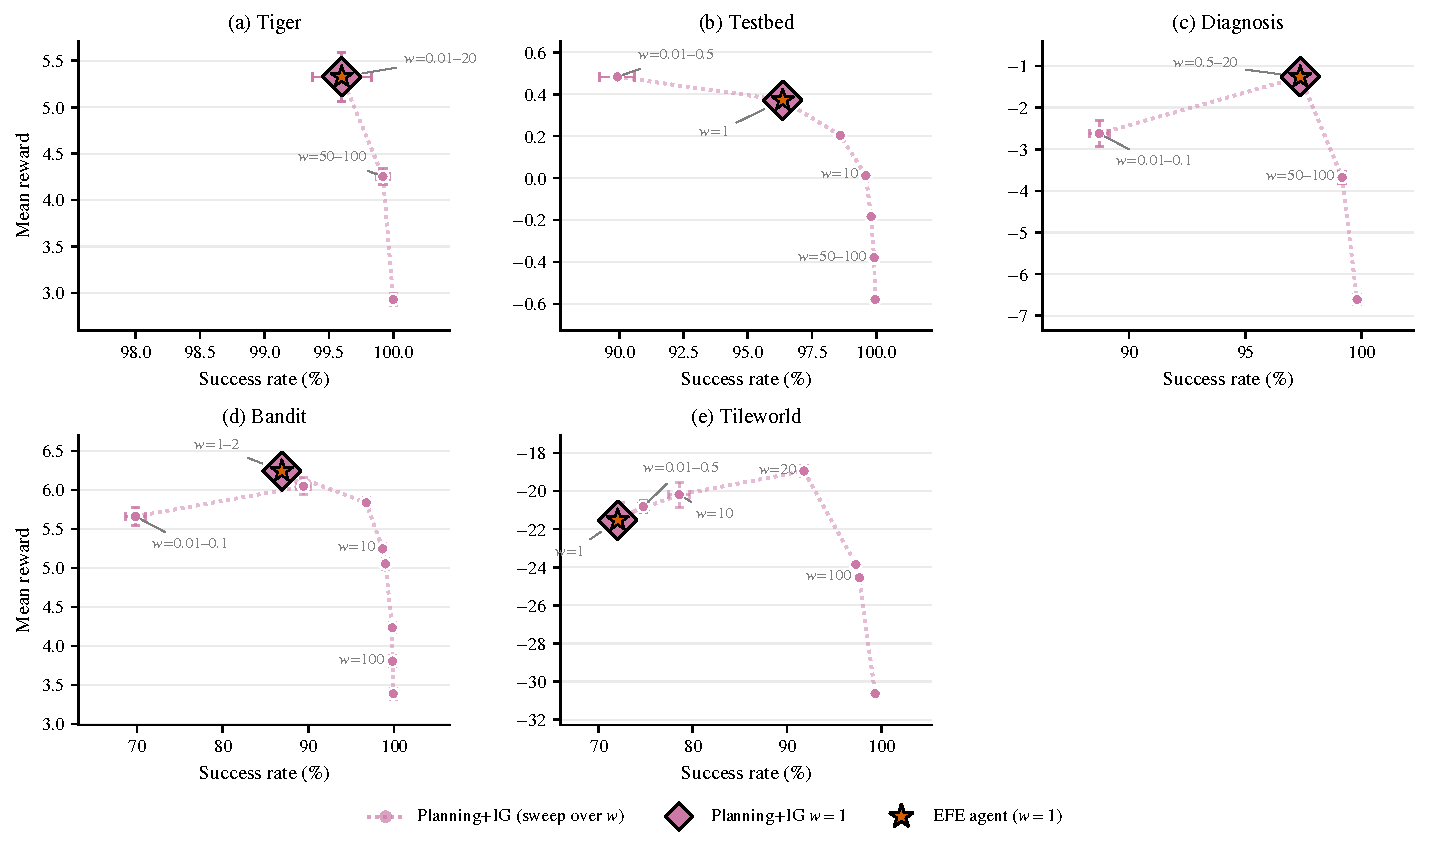
\includegraphics[width=\linewidth]{figures/fig_pareto.pdf}
\caption{Pareto analysis. Mean reward vs.\ success rate as $w$ varies from 0.01 to 200. The diamond marks Planning+IG at $w{=}1$ and the star marks the EFE agent. By Proposition~\ref{prop:equivalence} with shared deterministic tie-breaking, the markers coincide. On Tiger, Diagnosis, and Bandit the markers lie inside the reward-maximizing tied bracket. On Testbed they sit off it as a success-for-reward trade, and on Tileworld they are Pareto-dominated by $w{=}20$ on both axes (see text).}
\label{fig:pareto}
\Description{Five line plots arranged in a two by three grid, one per environment (Tiger, Testbed, Diagnosis, Bandit, Tileworld) with a legend in the sixth cell, each tracing mean reward against success rate as a pink dotted curve of connected dots swept over the info-gain weight, with weight labels from 0.01 to 100 along the points. On Diagnosis, Bandit, and Tileworld the curve rises to a knee and then bends sharply downward as success approaches 100 percent, while on Tiger and Testbed the curve only descends as success rises. A large pink diamond with a vermillion star inside sits on each curve, at the reward peak in the Tiger, Diagnosis, and Bandit panels, partway down the descent in the Testbed panel, and clearly down and to the left of the w equals 20 knee in the Tileworld panel.}
\end{figure}

On three of the five environments in the Pareto sweep, $w{=}1$ sits inside the reward-maximizing tied bracket, while the success-maximizing weight in the sweep lies at its upper endpoint, $w{=}200$, on all five environments. It sits outside that bracket on Testbed and is Pareto-dominated by $w{=}20$ on Tileworld (RockSample and Structural Inspection are not part of the sweep and are discussed separately in Sections~\ref{sec:rocksample} and~\ref{sec:inspection}). We emphasize that $w{=}1$ is near-optimal for reward on three of the five swept environments, not for success rate. Agents requiring near-certain accuracy (e.g., safety-critical applications) would benefit from higher weights at the cost of reduced reward. The contribution of EFE is deriving a principled weight from the variational objective that is near-optimal for reward maximization, rather than a grid search whose optimum changes by orders of magnitude across tasks.

\subsection{Tileworld: spatial epistemic foraging}
\label{sec:tileworld}

To test whether EFE's advantage extends to larger state spaces, we introduce a spatial generalization. The Tileworld projects the Diagnosis partition structure onto an $N{\times}N$ grid ($|S|{=}N^2$), producing spatially interpretable belief evolution (Figure~\ref{fig:tw_comparison}, with step-by-step belief strips in Appendix~\ref{app:tw_belief}).

\begin{table}[ht]
\centering
\caption{Tileworld $6{\times}6$ (2{,}500 episodes at 500 per seed $\times$ 5 seeds, $H{=}2$). Tuned weight $w^*_{\mathrm{succ}}{=}50$. Bold marks EFE and any agent not significantly different from it at the seed level (Welch $p > 0.05$, uncorrected), not the single best value per column.}
\label{tab:tileworld}
%% Numbers in this table are produced by experiments/run_tileworld.py all
\begin{small}
\begin{tabular}{lccc}
\toprule
Agent & Scans & Success & Reward \\
\midrule
Myopic & $0.00$ & 2.9\% & $-48.25$ \\
Planning ($H{=}2$) & $15.64$ & $\mathbf{73.8\%}$ & $\mathbf{-21.39}$ \\
Planning+IG ($w{=}50$) & $32.25$ & 97.3\% & $-23.85$ \\
\textbf{EFE} ($H{=}2$) & $\mathbf{14.75}$ & $\mathbf{72.0\%}$ & $\mathbf{-21.53}$ \\
\bottomrule
\end{tabular}
\end{small}
\end{table}

EFE and reward-only Planning are not significantly different on either reward ($-21.53$ vs.\ $-21.39$, seed-level Welch $p{=}0.82$, a failure to reject, not a TOST-backed equivalence claim) or success (72.0\% vs.\ 73.8\%, $p{=}0.17$, both bolded in Table~\ref{tab:tileworld}), but EFE reaches that outcome with significantly fewer scans (14.75 vs.\ 15.64, seed-level $p{=}8.8{\times}10^{-5}$, pooled $p<10^{-13}$). At this scale the epistemic bonus shows up in search cost rather than raw reward or success. Planning+IG's 32.25 scans, more than double EFE's, erode reward despite reaching 97.3\% success. The same over-exploration pattern from Diagnosis and Bandit recurs at this larger scale. Figure~\ref{fig:tw_comparison} visualizes the mechanism. EFE concentrates belief efficiently via partition-based narrowing and commits once confident, while Planning lacks scan-selection guidance and InfoGain-Tuned continues scanning past the point of diminishing returns.

\begin{figure}[t]
\centering
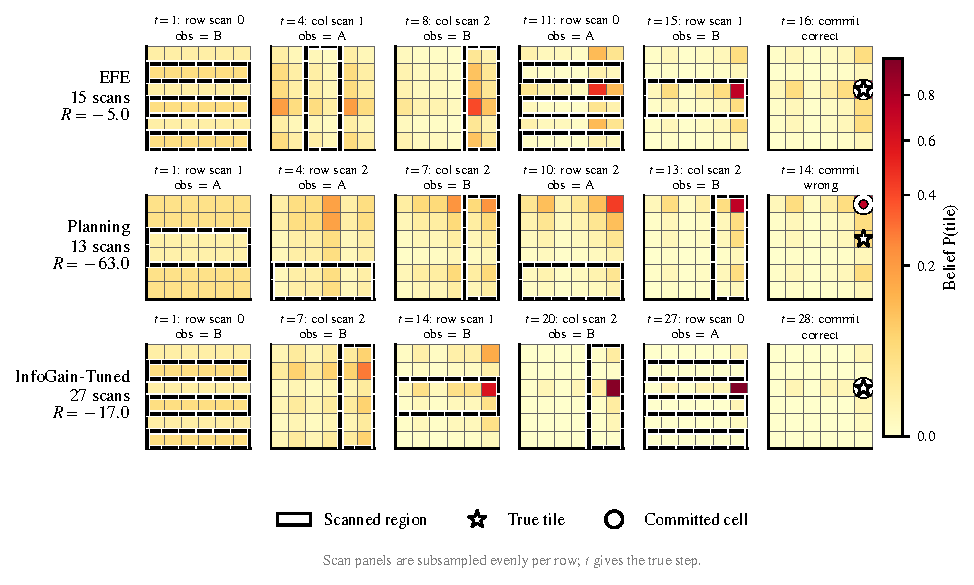
\includegraphics[width=\linewidth]{figures/fig_tileworld_comparison.pdf}
\caption{Agent comparison on the same $6{\times}6$ Tileworld episode. EFE (top) commits correctly with efficient scanning. Planning (middle) explores with less direction before committing. InfoGain-Tuned (bottom) over-scans well past the point of diminishing returns. The red circle marks the committed cell and the green star marks the target.}
\label{fig:tw_comparison}
\Description{Three rows of seven six-by-six grid heatmaps, one row per agent, showing numeric per-cell belief values that start uniform at 0.03. Blue rectangles outline the rows or columns scanned at each snapshot, and belief gradually concentrates into a single dark red cell. The top row ends with the circled commit cell coinciding with the star target after 15 scans. The middle row commits on a cell two rows above the star after 13 scans. The bottom row reaches a 0.98 belief on the correct cell but only after 27 scans.}
\end{figure}

\paragraph{Spatial scaling.} We scale the grid from $4{\times}4$ to $8{\times}8$ with five of the seven agents, omitting untuned Info Gain and EpistemicOnly (Figure~\ref{fig:tw_scaling}). At $8{\times}8$ ($|S|{=}64$), reward-only Planning collapses to $1.4\% \pm 0.3$pp success while EFE maintains $69.4\% \pm 1.0$pp (seed-level SE). The mechanism behind that contrast matters, because the headline number is easy to over-read. At $8{\times}8$ reward-only Planning takes zero scans and is bit-identical to Myopic on every outcome metric ($0.00$ scans, $1.4\%$ success, $-49.16$ reward for both). A single binary scan of a $64$-cell belief cannot repay its cost within an $H{=}2$ lookahead, so Planning never scans at all and the comparison at this scale is really EFE against a non-scanning agent. This is a joint horizon-and-scale effect at the fixed $H{=}2$ of this sweep, not evidence about reward-only planning at deeper horizons, where the scan would begin to pay for itself. Planning+IG at $w{=}100$ achieves $97.8\%$ success but at substantial reward cost due to extensive scanning. This reveals a nuanced picture. At $4{\times}4$ and $6{\times}6$, EFE's reward and success are within sampling error of reward-only Planning's (within 1 SE at both scales, with Planning nominally slightly ahead on both, no formal test was run for this specific sweep), and EFE's advantage opens up only at $8{\times}8$, exactly where Planning's success collapses. Planning+IG at $w{=}100$ achieves higher success rates at larger grids by exploring more, at a reward cost due to extensive scanning. The scaling sweep fixes $w{=}100$ for both weighted agents rather than tuning each in its own class as the main tables do, so this row is a fixed-weight comparison and not a tuned one. Safety-critical applications at large scale would therefore benefit from higher weights.

\begin{figure}[t]
\centering
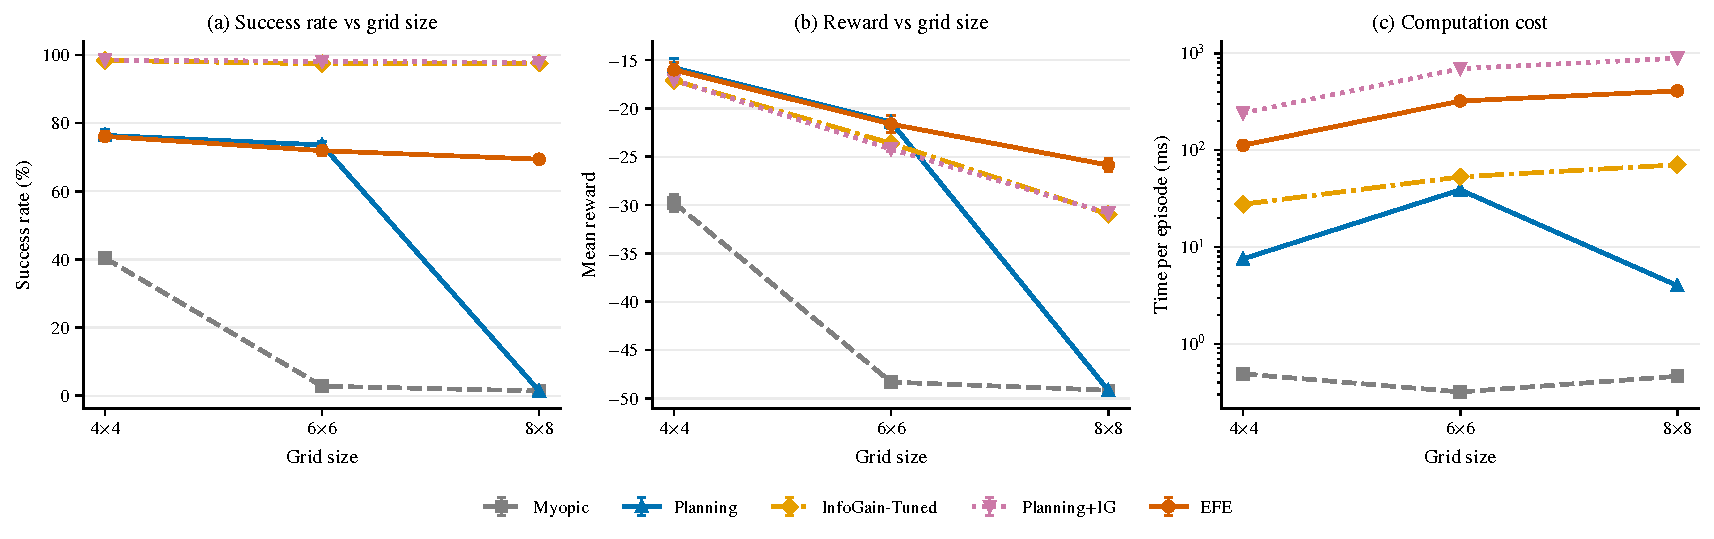
\includegraphics[width=\linewidth]{figures/fig_tileworld_scaling.pdf}
\caption{Tileworld scaling ($H{=}2$, 200 episodes per seed $\times$ 5 seeds) across Myopic, Planning, InfoGain-Tuned, Planning+IG, and EFE. Planning collapses at $8{\times}8$ ($|S|{=}64$), while EFE maintains $69.4\%$. Planning+IG at a fixed $w{=}100$, not tuned in class, achieves $97.8\%$ but at higher reward cost.}
\label{fig:tw_scaling}
\Description{Three line plots against grid sizes 4 by 4, 6 by 6, and 8 by 8. The left panel shows success rate, where the pink dotted Planning+IG and orange InfoGain-Tuned lines stay near 100 percent, the vermillion EFE line declines gently from about 76 to about 69 percent, the blue Planning line drops from about 76 percent to near zero at the largest grid, and the gray dashed Myopic line falls from about 40 percent to near zero by 6 by 6. The middle panel shows mean reward declining for all agents as grids grow, with the vermillion line ending highest near minus 26 and the blue and gray lines ending near minus 49. The right panel shows per-episode computation time on a log scale, where the pink line is highest and ends near 890 milliseconds, the vermillion line is next near 400 milliseconds, the orange line sits near 70 milliseconds, the blue line peaks near 40 milliseconds at 6 by 6 before falling to a few milliseconds, and the gray line is lowest below one millisecond.}
\end{figure}

\paragraph{Observation structure sensitivity.} A natural concern is whether EFE's advantage on Tileworld depends on the highly structured bit-level partition of scan actions. We test this by replacing the deterministic row/column splits with two alternative observation structures. Random partitions (each scan randomly assigns cells to two groups, breaking orthogonality) and overlapping partitions (scans use random linear combinations of coordinates, producing correlated and partially redundant observations). On $6{\times}6$ Tileworld ($H{=}2$, 200 episodes $\times$ 5 seeds, \texttt{results\_partition\_sensitivity\_6x6.csv}, \url{experiments/run_tileworld.py partition}), EFE against Planning in reward $\pm$ seed-level SE runs $-21.62 \pm 0.87$ (71.9\% success) vs.\ $-21.41 \pm 0.64$ (73.6\%) under the bitwise partition, $-29.31 \pm 0.43$ (56.1\%) vs.\ $-30.32 \pm 0.66$ (55.1\%) under the random partition, and $-47.53 \pm 0.73$ (8.5\%) vs.\ $-47.66 \pm 0.68$ (8.4\%) under the overlapping partition. No partition mode separates the two agents on reward at the seed level, the largest gap being $1.01$ reward under the random partition at $1.28$ seed-level SE of the difference (Welch $p{=}0.24$), and the nominal ordering itself changes direction across modes, with Planning nominally ahead under the bitwise partition and EFE nominally ahead under the random and overlapping ones. Planning is nominally ahead on success under the bitwise partition, but on success the two are within sampling error of each other under all three partition modes. The honest reading is that this battery does not resolve a Planning-versus-EFE ranking on reward or success under any partition structure. On scans, where the main $6{\times}6$ result lives, EFE stays ahead of Planning under all three modes ($14.76$ vs.\ $15.57$ bitwise, $12.97$ vs.\ $13.38$ random, $2.63$ vs.\ $2.70$ overlapping). An earlier unseeded version of this experiment showed EFE nominally ahead of Planning on reward under the bitwise partition, and the seeded rerun reverses that reward ordering, which is itself the clearest evidence that the nominal reward gaps here are sampling noise rather than signal. What the battery does establish is a large and consistent effect of observation structure on every agent. Both alternative modes cut absolute performance sharply, from roughly $-21$ reward under the bitwise partition to $-30$ under random scans and $-48$ under overlapping ones, because less complementary scans leave less recoverable information for any agent to exploit. We therefore treat the Tileworld result as scoped to the structured partition it was measured on, and we do not claim this experiment establishes EFE's advantage is model-independent.

\subsection{Interleaved observe-act: RockSample}
\label{sec:rocksample}

Proposition~\ref{prop:factored} covers check and navigation actions. To exercise that scope beyond observe-then-commit settings, we evaluate on a cost-modified variant of RockSample \citep{smith2004}, a widely used POMDP benchmark with interleaved observe-act dynamics (Section~\ref{sec:experiments} states the six deviations from the original). An agent navigates an $N{\times}N$ grid containing $K$ rocks at known positions, each with hidden binary quality. Actions include move (N/S/E/W, cost $-0.5$), check rock $k$ (noisy observation, accuracy decays with distance), sample (collect rock at current position, good $+10$, bad $-10$), and exit ($+10$). The Planning, Plan+IG, and EFE agents use depth-limited belief-space tree search over factored beliefs (independent per-rock), sharing one hand-coded leaf evaluation (\texttt{rho\_aif/agents/rocksample\_agents.py}) that, at the depth limit, greedily plans the remainder of the episode. It repeatedly moves to and samples the highest-scoring positive-expected-value unsampled rock, then exits. Because these three agents share that leaf value, they differ only in the information gain weight $w$.

% Auto-generated by experiments/build_rocksample_tables.py -- do not edit by hand.
\begin{table}[ht]
\centering
\caption{RockSample results. RS[5,3] and
 RS[7,4]: 500 episodes $\times$ 10 seeds (5{,}000 episodes). RS[7,8]
 and RS[11,11]: 100 episodes $\times$ 5 seeds (500 episodes, reduced
 protocol). Greedy samples without checking. POMCP is the genuine
 search-tree solver at its tuned, frozen configuration (2{,}048
 simulations, Appendix~\ref{app:rocksample}). Rollout only runs
 POMCP's approach-then-check rollout policy standalone, with no
 search tree. Bold marks the best mean reward per instance plus any
 agent not significantly different from it by a seed-level Welch
 $t$-test with Holm--Bonferroni correction, corrected within metric
 (complete pairwise statistics in the committed
 \texttt{results\_rocksample\_*\_stats.csv} files). Reward reported as mean $\pm$
 seed-level SE (SE of the per-seed means, RS[5,3]/RS[7,4]: 10 seeds;
 RS[7,8]/RS[11,11]: 5 seeds).
 Steps and Checks omitted here (per-instance step and check counts,
 and a Flat-MC(1000) reference on every instance, are in
 Appendix~\ref{app:rocksample}).}
\label{tab:rocksample}
\begin{small}
\begin{tabular}{llccc}
\toprule
Instance & Agent & Good & Bad & Reward \\
\midrule
\multirow{6}{*}{RS[5,3]}
 & Greedy & $1.49$ & $1.51$ & $+3.71 \pm 0.26$ \\
 & Planning ($w{=}0$, d=3) & $0.99$ & $0.04$ & $+14.28 \pm 0.13$ \\
 & Plan+IG ($w{=}5$, d=3) & $1.44$ & $0.01$ & $\mathbf{+16.41 \pm 0.13}$ \\
 & EFE ($w{=}1$, d=3) & $1.44$ & $0.03$ & $\mathbf{+16.47 \pm 0.12}$ \\
 & POMCP (2048 sims) & $0.68$ & $0.03$ & $+12.74 \pm 0.11$ \\
 & Rollout only (approach) & $1.41$ & $0.07$ & $\mathbf{+16.67 \pm 0.13}$ \\
\midrule
\multirow{6}{*}{RS[7,4]}
 & Greedy & $1.98$ & $2.02$ & $-1.38 \pm 0.36$ \\
 & Planning ($w{=}0$, d=4) & $0.95$ & $0.05$ & $+13.97 \pm 0.11$ \\
 & Plan+IG ($w{=}5$, d=4) & $1.69$ & $0.01$ & $+14.56 \pm 0.14$ \\
 & EFE ($w{=}1$, d=4) & $1.44$ & $0.01$ & $\mathbf{+15.96 \pm 0.15}$ \\
 & POMCP (2048 sims) & $0.66$ & $0.03$ & $+12.01 \pm 0.06$ \\
 & Rollout only (approach) & $1.88$ & $0.10$ & $\mathbf{+15.85 \pm 0.17}$ \\
\midrule
\multirow{6}{*}{RS[7,8]}
 & Greedy & $4.02$ & $3.98$ & $-5.60 \pm 1.03$ \\
 & Planning ($w{=}0$, d=3) & $0.48$ & $0.03$ & $+12.31 \pm 0.35$ \\
 & Plan+IG ($w{=}5$, d=3) & $3.40$ & $0.01$ & $+23.76 \pm 0.58$ \\
 & EFE ($w{=}1$, d=3) & $2.61$ & $0.06$ & $+21.85 \pm 0.79$ \\
 & POMCP (2048 sims) & $1.71$ & $0.10$ & $+15.07 \pm 0.45$ \\
 & Rollout only (approach) & $3.83$ & $0.19$ & $\mathbf{+28.33 \pm 0.82}$ \\
\midrule
\multirow{6}{*}{RS[11,11]}
 & Greedy & $5.48$ & $5.52$ & $-18.90 \pm 1.04$ \\
 & Planning ($w{=}0$, d=2) & $0.48$ & $0.03$ & $+13.23 \pm 0.18$ \\
 & Plan+IG ($w{=}5$, d=2) & $0.50$ & $0.03$ & $+13.18 \pm 0.15$ \\
 & EFE ($w{=}1$, d=2) & $0.48$ & $0.03$ & $+13.23 \pm 0.18$ \\
 & POMCP (2048 sims) & $0.49$ & $0.03$ & $+12.94 \pm 0.24$ \\
 & Rollout only (approach) & $5.22$ & $0.23$ & $\mathbf{+28.66 \pm 0.83}$ \\
\bottomrule
\end{tabular}
\end{small}
\end{table}


On RS[5,3], EFE and Plan+IG ($w{=}5$) are not significantly different ($+16.47$ vs.\ $+16.41$, seed-level Welch $p{=}0.74$, a failure to reject, not a TOST-backed equivalence claim), and both are bolded in Table~\ref{tab:rocksample} as statistical ties with the best row, which is the standalone heuristic at $+16.67$. On RS[7,4], EFE leads the weighted family outright ($+15.96$ vs.\ $+14.56$ for Plan+IG, $p<10^{-5}$) and is statistically tied with the heuristic's $+15.85$ ($p{=}0.65$, again a failure to reject rather than demonstrated equivalence). On RS[7,8], EFE and Plan+IG ($w{=}5$) are again not significantly different from each other ($+21.85$ vs.\ $+23.76$, $p{=}0.09$ uncorrected, not significant after Holm--Bonferroni), while both substantially outperform Planning ($+12.31$, $p<10^{-4}$). Against the heuristic's $+28.33$, both deficits survive the per-metric Holm correction (Plan+IG $p{=}2.4{\times}10^{-3}$, EFE $p{=}4.6{\times}10^{-4}$), so the table bolds the heuristic alone there. All three sit below the $+28.33 \pm 0.82$ reached by the unbounded-horizon approach-then-check heuristic on the identical protocol, so these are relative comparisons within a family that is jointly suboptimal on this instance. More checking beyond $w{=}5$ never significantly helps across these three instances, and twice significantly hurts. Plan+IG ($w{=}10$, Appendix~\ref{app:rocksample}) falls to $+20.55$ here ($p{=}0.003$, significant under the per-metric Holm family). The drop at RS[5,3] is decisive ($+14.60$ vs.\ $+16.41$, $p{=}3.5{\times}10^{-9}$), while at RS[7,4] the same step is flat ($p{=}0.18$) because EFE had already beaten both tuned weights outright from $w{=}1$. So among the weights we ran on RS[7,8], $w{=}5$ attains the highest reward, and it is not significantly different from $w{=}1$. We ran only $w \in \{5, 10\}$ as tuned comparators on RockSample, not the nine-point grid used for the observe-then-commit environments (Section~\ref{sec:methodology}), so this identifies the best of three sampled weights rather than a grid-searched argmax, and we make no claim that $w{=}5$ is the reward-maximizing weight over a denser sweep. The gap vs.\ $w{=}0$ Planning is largest on RS[7,8] among these three instances, though it does not extend to RS[11,11] below, where it vanishes entirely despite that instance having the most rocks to check. On RS[5,3], RS[7,4], and RS[7,8], EFE samples dramatically fewer bad rocks than Greedy ($0.01$--$0.06 \pm 0.001$--$0.013$ vs.\ $1.51$--$3.98 \pm 0.01$--$0.05$, seed-level SE, seed-level Welch $p<5{\times}10^{-8}$ at every instance), confirming that the information gain term drives checking behavior.

On RS[11,11] ($|S|{=}2{,}048$), EFE and Planning achieve identical reward ($+13.23$ each). Every tree-search agent vastly outperforms Greedy ($+12.9$ to $+13.2$ against $-18.9$), but nothing here differentiates EFE from reward-only planning. Every tree-search agent at its reported configuration, POMCP at its frozen setting included, converges to the same conservative pattern of checking one or two nearby rocks, sampling if a rock looks good, and exiting, so the weight on information gain moves reward by at most $0.06$. Moving from depth 2 to depth 3 does not change this. Rerunning at depth 3 (\texttt{results\_rocksample\_11x11\_depth3\_check.csv}) costs seconds and reproduces the same $+13.23$ and $+13.17$ pattern within 1 SE.

Two explanations fit that collapse. Either the instance leaves no exploitable slack, so every agent is already near the ceiling, or it leaves a great deal of slack that no depth-limited search can reach. A reference agent added for the POMCP comparison settles which one holds, and the answer is not the flattering one. The approach-then-check heuristic that serves as POMCP's rollout policy is a hand-coded, unbounded-horizon rule. It walks to the unresolved rock with the highest belief per unit of distance (the nearest one at a uniform prior), checks it at close range where accuracy is $0.95$, samples if the belief crosses a threshold, writes off any rock whose belief falls below $0.15$, and exits when nothing is left. Run standalone on the same $5$ seeds and $100$ episodes as the table above, it scores $+28.66 \pm 0.83$ on RS[11,11], where every tree-search agent, EFE and POMCP included, sits in the $+12.94$ to $+13.23$ band. On RS[7,8] it scores $+28.33 \pm 0.82$ against the best tree-search agent's $+23.76 \pm 0.58$.

So the first explanation fails. There is no shortage of slack at 11 widely spaced rocks. There is a great deal of it, and the depth-limited belief-space search cannot reach it. The mechanism is now identifiable. At this instance the informative checks are far from the agent, and a depth-2 or depth-3 tree cannot represent the walk that makes them informative, so within its horizon only a single check taken from the agent's own starting cell is worth making and the weight on information gain has almost nothing to act on. The shared greedy leaf heuristic values a rock at its belief-weighted sample reward, which is exactly zero at the uniform prior, so it recommends the exit. One further detail of that leaf deserves disclosure. Its completion estimate charges move costs for a walk to the east edge before collecting the exit reward (\texttt{rocksample\_agents.py}), while the environment pays the exit from any cell. The phantom travel cost deflates every depth-capped continuation relative to the exact value of exiting immediately, a bias toward earlier exits. Every agent in the family shares it identically, so within-family comparisons are unaffected, but it means the leaf's exit recommendation is overdetermined here rather than resting on the zero prior expectation alone. That is why depth 3 leaves reward unchanged and why every weight gives the same reward to within $0.06$, with the higher weights buying only about half an extra check per episode. POMCP corroborates the mechanism from the other side. Given horizon enough to reach the distant checks, its reward falls monotonically, from $+12.94$ at $H{=}10$ to $-54.78$ at $H{=}40$, because the tours it assembles from noisy distant checks do not pay (Appendix~\ref{app:rocksample}).

This is a limitation of the tree-search family at feasible depths on this instance, not evidence about information-gain weighting, and it bounds what RockSample[11,11] can be asked to show about EFE. It also sharpens the honest scope of the comparison. On the two larger instances our agents are competing against each other well below what a simple unbounded-horizon rule achieves. Per-instance detail, including the Flat-MC reference and the standalone heuristic on every instance, is in Appendix~\ref{app:rocksample}.

Read together with Tileworld and RS[7,8], these are one mechanism seen at three points rather than three unrelated per-instance results. EFE's advantage over reward-only Planning tracks how far the reward-only policy's default behavior already sits from the information-optimal one. On Tileworld, reward-only Planning scans too little to disambiguate a large grid, so directed information gain buys a large success-rate margin. On RS[7,8], eight rocks spread across a mid-sized grid leave real ambiguity about which are worth sampling, so choosing which rock to check pays off. On RS[11,11] the rocks sit far enough apart that no check beyond the agent's own cell is worth taking within the depths we run, so the weight has almost nothing to act on and every tree-search agent collapses to an early exit after one or two checks, far below what an unbounded-horizon heuristic achieves. The prediction this yields is that EFE's advantage should track how much slack a problem's structure leaves between the reward-only policy and the information-optimal one that the agent's search can actually represent, not problem size or agent count in themselves. We did not design or run instances specifically to stress-test that prediction, so it remains a mechanistic reading of the four RockSample instances and three Tileworld scales already reported rather than an independently validated scaling law.

\subsection{Structural inspection}
\label{sec:inspection}

To exercise Proposition~\ref{prop:factored}'s scope on a domain-realistic benchmark and demonstrate scalability beyond existing environments, we implement a Structural Inspection POMDP mapping directly to industrial fault detection, medical screening, and non-destructive testing domains. The agent inspects $N$ components arranged spatially, each with a hidden binary state (nominal/faulty). Two non-destructive test types provide accuracy--cost trade-offs, a visual check (accuracy 0.70, cost 0.5) and a detailed test (accuracy 0.90, cost 2.0). The agent navigates between components, selects tests, and declares diagnoses with asymmetric penalties (missed fault $-50$, false alarm $-5$). Tests do not alter component states, so this is a factored observation POMDP and Proposition~\ref{prop:factored} applies. As on RockSample, all tree-search agents here share one hand-coded leaf evaluation (\texttt{rho\_aif/agents/inspection\_agents.py}) that greedily completes the episode from the depth limit, so agents in this section differ only in the information-gain weight and not in their leaf value.

\begin{table}[ht]
\centering
\caption{Structural Inspection results. $N{=}8$ and $N{=}16$ run 2{,}500 episodes each (500 per seed $\times$ 5 seeds). Reward and accuracy are reported as mean $\pm$ seed-level SE, the SE of the 5 per-seed means. Greedy diagnoses without testing. Bold marks the best accuracy and the best reward per instance, plus any value within sampling error of that best (seed-level Welch $p > 0.05$, uncorrected). The two are not always the same agent. EFE is a competitive untuned trade-off, not uniquely best on all metrics. Accuracy is the fraction of components correctly diagnosed.}
\label{tab:inspection}
%% Numbers in this table are produced by experiments/run_inspection.py
\begin{small}
\begin{tabular}{llcccc}
\toprule
Instance & Agent & Accuracy & Missed & Tests & Reward \\
\midrule
\multirow{4}{*}{\shortstack[l]{$N{=}8$\\[-1pt]{\scriptsize $|S|{=}256$}}} & Greedy & $70.7 \pm 0.5\%$ & $2.34$ & $0.0$ & $-114.33 \pm 1.96$ \\
& Planning ($w{=}0$) & $73.0 \pm 0.3\%$ & $0.07$ & $12.7$ & $\mathbf{-17.85 \pm 0.23}$ \\
& Planning+IG ($w{=}5$) & $\mathbf{96.3 \pm 0.1\%}$ & $0.10$ & $19.7$ & $-27.98 \pm 0.44$ \\
& EFE ($w{=}1$) & $91.1 \pm 0.2\%$ & $0.09$ & $15.5$ & $-20.95 \pm 0.30$ \\
\midrule
\multirow{4}{*}{\shortstack[l]{$N{=}16$\\[-1pt]{\scriptsize $|S|{=}65{,}536$}}} & Greedy & $70.5 \pm 0.4\%$ & $4.72$ & $0.0$ & $-233.09 \pm 3.13$ \\
& Planning ($w{=}0$) & $78.2 \pm 0.2\%$ & $0.24$ & $22.4$ & $\mathbf{-45.42 \pm 0.23}$ \\
& Planning+IG ($w{=}5$) & $\mathbf{97.3 \pm 0.0\%}$ & $0.14$ & $38.3$ & $-54.74 \pm 0.40$ \\
& EFE ($w{=}1$) & $90.8 \pm 0.1\%$ & $0.24$ & $28.1$ & $\mathbf{-45.80 \pm 0.60}$ \\
\bottomrule
\end{tabular}
\end{small}
\end{table}

EFE ($w{=}1$) is a competitive untuned trade-off rather than uniquely best. On $N{=}8$ ($|S|{=}256$), Planning wins reward ($-17.85$), while EFE achieves $91.1\%$ accuracy ($-20.95 \pm 0.30$), gaining $+18.0$pp accuracy over Planning ($73.0\%$, seed-level Welch $p<10^{-10}$) at a moderate reward cost. Planning+IG ($w{=}5$) reaches $96.3\%$ accuracy but at $-27.98$ reward, over-testing relative to reward. On $N{=}16$ ($|S|{=}65{,}536$), Planning posts the best mean reward ($-45.42$, with EFE a close second at $-45.80$ whose deficit is not significant, seed-level $p{=}0.57$, so the two reward cells are bolded together), while Planning+IG ($w{=}5$) wins accuracy ($97.3\%$) at substantial reward cost ($-54.74$, the worst of the three informed agents) from extensive over-testing ($38.3 \pm 0.05$ tests vs.\ EFE's $28.1 \pm 0.09$, seed-level SE, roughly $36\%$ more, seed-level Welch $p{=}1.7{\times}10^{-11}$). EFE outperforms Planning by $+12.6$pp accuracy ($90.8\%$ vs.\ $78.2\%$, seed-level $p<10^{-7}$) at a reward cost of only $0.39$ that is itself not significant, a far better accuracy-per-reward trade than Planning+IG's. This is the largest state space in our evaluation and confirms that the factored belief tree search scales to realistic domains. The penalty structure is asymmetric on the missed-fault side. Declaring nominal pays $+2$ when correct and $-50$ when a fault is missed ($\alpha = 25$ for that decision), while declaring a fault is symmetric ($+5$ when correct, $-5$ on a false alarm, $\alpha = 1$). Reading Proposition~\ref{prop:nearopt}'s two-state thresholds onto this multi-state environment is a heuristic reduction, as with the two-state-reduced rows of Table~\ref{tab:alpha_eta}, and on the missed-fault side, where the large penalty sits, that reading places the environment in the regime where the proposition predicts $w{=}1$ is a reasonable untuned default.

\subsection{Summary}

Taken together, the experiments tell a consistent story. The behavior predicted by Propositions~\ref{prop:equivalence} and~\ref{prop:factored} is what we observe. EFE matches Planning+IG at $w{=}1$ within their stated scope, and that information-unit weight lands inside the reward-maximizing bracket on three of the five swept environments without per-environment search. Where multiple observation actions matter most, as on Diagnosis and Bandit, untuned EFE Pareto-dominates same-horizon planning. Where tuned bonuses chase success harder, they can beat EFE on accuracy at a reward cost. Across Tileworld, RockSample, and Inspection, EFE remains a competitive untuned trade-off rather than uniquely best on every metric. The advantage over $w{=}0$ Planning opens at the largest scale of the Tileworld sweep (Figure~\ref{fig:tw_scaling}), and it is not a general size pattern. It vanishes entirely on RockSample[11,11] despite that instance having the most rocks to check, and on Structural Inspection the accuracy advantage narrows from $+18.0$pp at $N{=}8$ ($|S|{=}256$) to $+12.6$pp at $N{=}16$ ($|S|{=}65{,}536$) even as its reward cost narrows in parallel.

\section{Experiments: shadow prices and sensing budgets}
\label{sec:budget_experiments}

Section~\ref{sec:results} evaluated the equivalence and near-optimality claims of Sections~\ref{sec:methodology}--\ref{sec:experiments}. This section evaluates the budgeted reformulation of Section~\ref{sec:budget}. It covers usage-curve collapse across reward scales, closed-form onset recovery, online tracking through a reward rescale, cost-denominated budgets, interleaved (non-observe-then-commit) settings, a near-optimal offline reference, an atlas of implicit budgets, and an explicit test of what the budget does and does not fix. All headline runs use five seeds $\{42,123,456,789,1024\}$ and $100$ episodes per evaluation cell unless noted. The tree-search cells are the noted exceptions, their per-episode cost being an order of magnitude higher than the observe-then-commit domains. Tileworld-$6{\times}6$ runs $40$ episodes per usage-curve cell and $30$ per scale-collapse cell, and Inspection-$N{=}8$ runs $30$ per usage-curve cell. Code and CSVs accompany the repository.

\subsection{Curve collapse across reward scales}
\label{sec:collapse}

On Diagnosis and Bandit we estimate $U(w;\alpha)$ at reward scales $\alpha \in \{0.1, 1, 10\}$ on $\alpha$-scaled weight grids so that $w/\alpha$ abscissae align. Figure~\ref{fig:collapse} shows the curves collapsing on Diagnosis. Every matched $w/\alpha$ point coincides exactly across scales (bit-exact, not merely within $2\cdot\mathrm{SE}$, under the per-episode seeded pipeline), and the crossing bracket of budget $B{=}8$ in $w/\alpha$ units coincides across $\alpha$ ($(0.141, 0.323]$ at every scale). We extend the check to Tiger and Tileworld-$6{\times}6$ to avoid resting the headline claim on two environments (Table~\ref{tab:collapse-breadth}).

\begin{figure}[t]
\centering
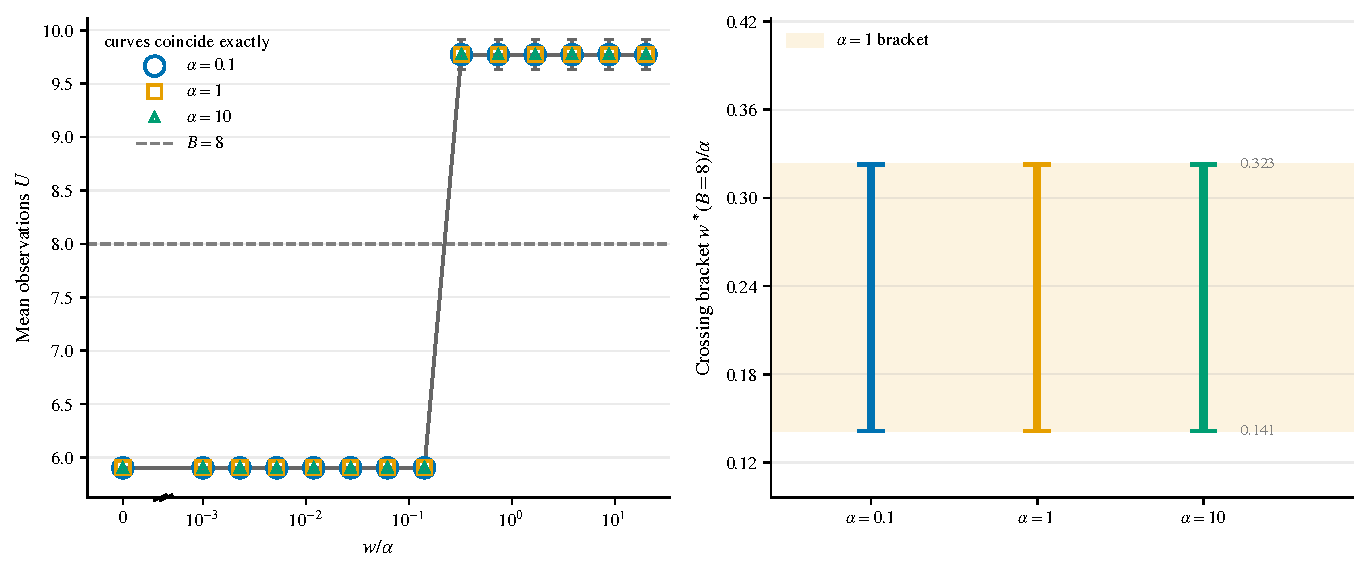
\includegraphics[width=0.85\textwidth]{figures/price_scale_invariance.pdf}
\caption{Curve collapse on Diagnosis. The left panel plots $U$ against $w/\alpha$ at three reward scales. The right panel shows crossing brackets of $B{=}8$ in $w/\alpha$ units coinciding across scales, a set-valued shadow price.}
\label{fig:collapse}
\Description{Two panels. Left: mean observations against the ratio of w to alpha on a log-style axis, with three overlapping error-bar curves in blue, orange, and green that stay flat near 6, jump steeply to about 10 near a ratio of 0.2, and stay flat thereafter. A gray dashed horizontal line at 8 crosses inside the jump. Right: three identical vertical interval bars at alpha equals 0.1, 1, and 10, all spanning the same range of the ratio axis, with a shaded band marking the alpha equals 1 bracket.}
\end{figure}

\begin{table}[t]
\centering
\caption{Curve-collapse breadth. Fraction of matched $w/\alpha$ points across $\alpha \in \{0.1,1,10\}$ within $2\cdot\mathrm{SE}$, and whether the $B$-crossing bracket coincides across scales (in $w/\alpha$ units).}
\label{tab:collapse-breadth}
%% Numbers in this table are produced by experiments/run_price_of_information.py --mode full --only scale
\small
\begin{tabular}{lccp{4.3cm}}
\toprule
Environment & Within $2\cdot\mathrm{SE}$ & Max spread & Bracket at $B$ \\
\midrule
Diagnosis ($B{=}8$) & $100\%$ & $0.00$ obs.\ (bit-exact) & $(0.141, 0.323]$ at every $\alpha$ \\
Bandit ($B{=}8$) & $100\%$ & $0.00$ obs.\ (bit-exact) & $(3.84, 8.76]$ at every $\alpha$ \\
Tiger ($B{=}4$) & $100\%$ (trivial) & $0.00$ obs.\ (bit-exact) & unbracketed ($B$ below observed $U$ at every $\alpha$) \\
Tileworld-$6{\times}6$ ($B{=}15$) & $100\%$ & $0.00$ obs.\ (bit-exact) & $(5.80, 20.0]$ at every $\alpha$ \\
\bottomrule
\end{tabular}
\end{table}

Every environment shows bit-exact collapse. Every matched $w/\alpha$ point coincides exactly across the three scales, not merely within Monte Carlo tolerance, and every crossing bracket coincides across scales down to floating-point noise ($\le 10^{-15}$). This is the strongest form the check can take, and it is available only because environment streams are seeded per episode, which makes Proposition~\ref{prop:pi1}'s theorem an exact empirical replay rather than an approximate one. Diagnosis and Bandit exhibit the exact collapse the proposition guarantees. Tiger passes trivially. Instrumental listening already saturates usage (constant $4.37$ observations at every grid point) across the entire $w/\alpha \in [0,20]$ range tested, so the budget formulation has no usable dial in this window. Proposition~\ref{prop:pi1} guarantees collapse of whatever curve there is, not that every environment has an informative curve to collapse. Tileworld-$6{\times}6$'s bracket coincides exactly at $(5.80, 20.0]$ for every scale.

\subsection{Proposition~\ref{prop:nearopt} onset on positive-threshold testbeds}
\label{sec:prop2exp}

Standard Tiger and Testbed parameters yield negative $w_{\mathrm{thresh}}$, so any $w \ge 0$ observes and the duality check of Corollary~\ref{cor:pi4} is vacuous there. We therefore construct positive-threshold InfoSeeking environments ($p \in \{0.60, 0.58\}$, $c{=}0.3$, $R_\pm = \pm 1$) with closed forms $w_{\mathrm{thresh}} \approx 3.44$ and $7.55$ in the implementation's bit units, which is the convention the swept weight grid uses, equivalently $4.97$ and $10.89$ nats. A refined weight grid around the threshold shows $U{=}0$ at and below $w_{\mathrm{thresh}}$, with onset in $(w_{\mathrm{thresh}}, 1.03\cdot w_{\mathrm{thresh}}]$ on both environments (upper relative error $3\%$, Figure~\ref{fig:prop2}), matching Corollary~\ref{cor:pi4}. Negative-threshold sanity checks on standard Testbed and Tiger remain consistent ($U(0) > 0$ when $w_{\mathrm{thresh}} < 0$).

\begin{figure}[t]
\centering
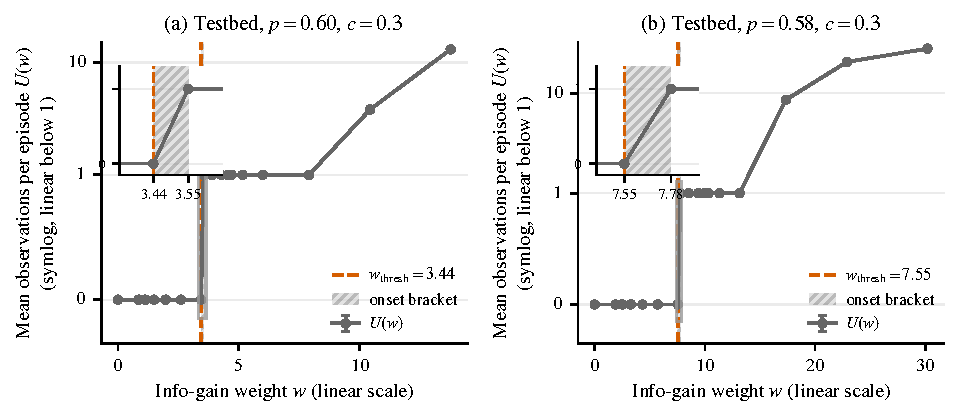
\includegraphics[width=\textwidth]{figures/price_prop2_jumps.pdf}
\caption{Onset of observing on positive-threshold testbeds. The orange dashed vertical line marks the $H{=}1$ closed-form threshold (Proposition~\ref{prop:nearopt}) and the green band is the empirical onset bracket after grid refinement.}
\label{fig:prop2}
\Description{Two panels of mean observations versus the weight w, each showing a blue solid curve with round markers that sits at zero, steps up to one just past an orange dashed vertical threshold line with a thin green onset band, plateaus at one, and then climbs steeply at large weights to about 13 in the left panel and about 28 in the right panel. The threshold lines sit near w equals 3.4 on the left and 7.6 on the right.}
\end{figure}

\subsection{Multi-seed online dual control under reward rescale}
\label{sec:dual_multiseed}

On Diagnosis with target $B{=}8$, learning rate $\eta_0{=}0.05$, decay $\delta{=}0.02$, and a $\times 10$ reward-and-cost rescale at episode~$200$ of a $400$-episode run, we sweep $10$ independent controller seeds for decay-only and reset-on-shift variants (window~$20$, $k{=}3$, absolute floor $0.5$), extending the single-trajectory workshop result to a multi-seed comparison with confidence intervals. Re-adaptation is measured as episodes from rescale until rolling-20 usage, computed strictly from post-rescale episodes only, stays within $\pm 1$ of $B$ for $20$ consecutive episodes. Restricting the window to post-rescale episodes matters. A window allowed to straddle the rescale point reports a spuriously fast recovery by mixing in already-converged pre-rescale usage (\texttt{experiments/run\_price\_of\_information.py:\allowbreak readaptation\_episodes}). Under the corrected metric, decay-only recovery averages $150.9$ episodes, $95\%$ CI $[142.9, 158.9]$ (normal-approximation CIs throughout this analysis), with $10/10$ seeds recovering inside the $200$ post-rescale episodes. Reset-on-shift mean $57.0$, CI $[52.0, 62.0]$, $10/10$ recovered, all but one seed triggering exactly one learning-rate reset (one seed triggers two). The CIs are disjoint, and reset-on-shift re-adapts roughly $2.65\times$ faster than decay alone. Post-rescale steady-state $|U-B|$ is $0.10$ ($[0.056,0.144]$) under reset versus $0.19$ ($[0.061,0.323]$) under decay-only. Pre-rescale steady-state error is $0.15$ ($[0.095,0.209]$) for both variants (identical, since decay and reset only diverge after the rescale), close to the tolerance used to declare recovery. Figure~\ref{fig:dualmultiseed} shows the median trajectory with interquartile band for both variants.

\begin{figure}[t]
\centering
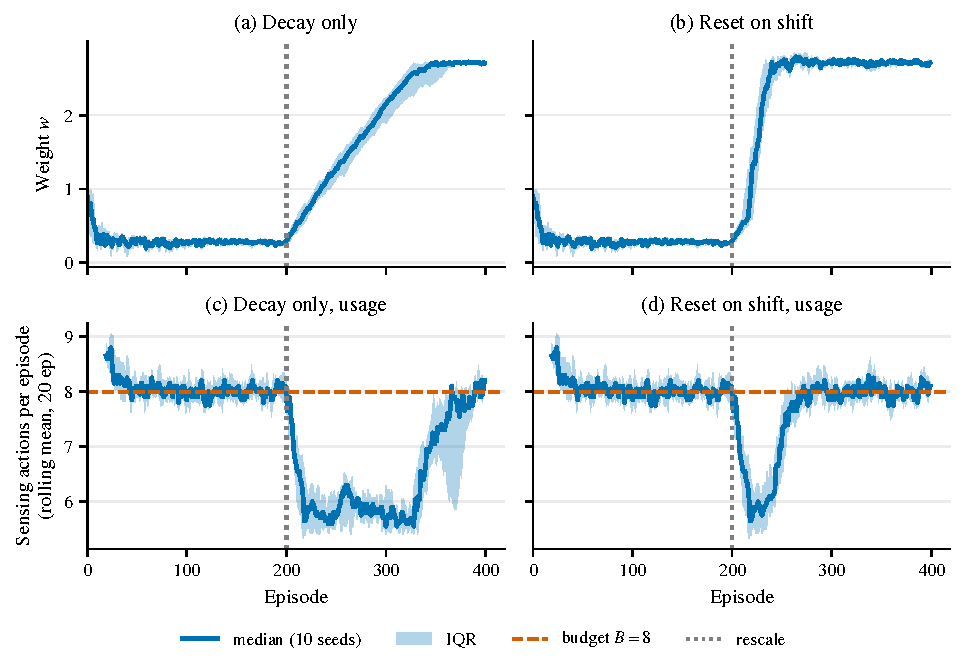
\includegraphics[width=0.85\textwidth]{figures/price_dual_multiseed.pdf}
\caption{Multi-seed ($n{=}10$) dual control of $w$ on Diagnosis through a mid-run $\times 10$ reward rescale (vertical line). Median trajectory with interquartile band. Decay-only (left) vs.\ reset-on-shift (right). Reset-on-shift re-adapts in a mean of $57$ episodes vs.\ $151$ for decay alone (post-shift-only rolling window), with disjoint 95\% CIs.}
\label{fig:dualmultiseed}
\Description{A two-by-two grid of time series over 400 episodes, with one column per controller variant. Top row. The median weight trajectory with a shaded interquartile band drops from about 1 to about 0.3, holds flat until the dotted vertical line at episode 200, then climbs to about 2.7. The left variant climbs gradually over roughly 150 episodes while the right variant jumps up within about 50 episodes. Bottom row: rolling median usage hovers on the dashed budget line at 8, dips to between about 5 and 6 after the shift, and returns to the budget line, slowly on the left and quickly on the right.}
\end{figure}

The multi-seed result strengthens rather than merely replicates the single-trajectory workshop finding. Under the corrected pipeline, both variants recover on all $10$ seeds tested within the $200$-episode post-rescale window, but decay-only takes roughly $2.65\times$ longer on average and reaches a looser post-rescale steady state, whereas reset-on-shift recovers faster on every seed and reaches a tighter post-rescale steady state on six of the ten seeds. Both arms run the decaying step of Equation~\ref{eq:dual_update} at $\delta{=}0.02$, so this is nonstationary re-adaptation outside Proposition~\ref{prop:pi5}'s stationary scope. The mechanism is the residual step size that the constant-step discussion after Proposition~\ref{prop:pi5} identifies. At the rescale episode the decayed step is still large enough to move the iterate. The proposition's stationary convergence guarantee is not being tested here, since the environment is deliberately shifted mid-run.

\subsection{Cost-denominated budgets}
\label{sec:cost_budget}

The count-usage curves above treat every observation as one unit regardless of price. To demonstrate the units story end to end, we introduce a Diagnosis variant with heterogeneous per-test costs ($[0.5, 2.5]$ across the two test types, same accuracy) and estimate both the count-usage curve $U_{\mathrm{count}}(w)$ and the cost-usage curve $U_{\mathrm{cost}}(w)$ on the same agent family. The mean cost paid per test, $U_{\mathrm{cost}}(w)/U_{\mathrm{count}}(w)$, is not constant. It varies from $1.26$ to $1.41$ across the weight grid, a $12.0\%$ spread relative to the grid-mean cost per test, rising as high $w$ pushes the agent onto relatively more of the expensive test. This confirms the units story directly. A count budget cannot see that the agent's test mix shifts toward the more expensive test as $w$ rises, while a cost budget prices that shift. At the two comparable operating points we solve for, however, the two denominations happen to land in the same crossing bracket at this grid's resolution. A count budget $B{=}8.86$ brackets $w^*$ in $(10, 31.6]$, and a cost budget $B_{\mathrm{cost}}{=}11.50$ (a comparable operating point in dollars-of-sensing rather than test-count) also brackets $w^*$ in $(10, 31.6]$ (Figure~\ref{fig:costbudget}). The same coincidence holds at the higher pair of budgets we test ($B{=}13.71$ count, $B_{\mathrm{cost}}{=}19.20$ cost, both bracketing $w^*$ in $(31.6, 100]$). With a $12\%$ cost-ratio spread and log-spaced grid knots roughly $2$--$3\times$ apart, the two denominations are not guaranteed to disagree at every tested budget pair, only to disagree in general when the ratio's variation is large enough relative to the grid's resolution.

\begin{figure}[t]
\centering
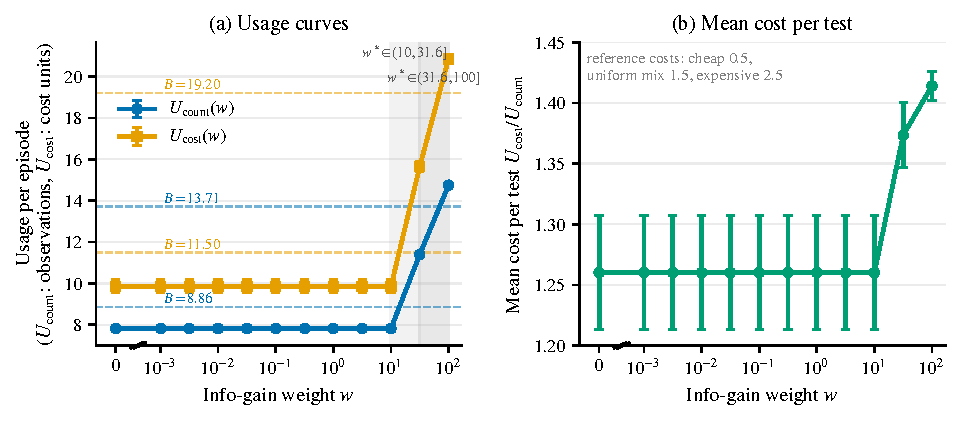
\includegraphics[width=0.85\textwidth]{figures/price_cost_budget.pdf}
\caption{Cost- vs.\ count-denominated usage curves on heterogeneous-cost Diagnosis. The two curves disagree because sensing cost per test is not constant across $w$, while their crossing brackets happen to coincide at both tested budget pairs.}
\label{fig:costbudget}
\Description{Two panels versus the info-gain weight on a log axis. The left panel has two error-bar curves, a blue count-usage curve flat near 7.5 to 8 and an orange cost-usage curve flat near 9.5 to 10, both rising sharply beyond a weight of 10 to about 15 and 21 respectively, with the gap between them widening. The right panel has a green curve of mean cost per test that stays between about 1.26 and 1.41, sitting between dashed reference lines for the cheap test at 0.5, a uniform mix at 1.5, and the expensive test at 2.5, and drifting slightly upward at the largest weights.}
\end{figure}

\subsection{Interleaved settings: RockSample and Structural Inspection}
\label{sec:interleaved_budget}

The observe-then-commit environments above cannot exercise every structural feature of Proposition~\ref{prop:factored}'s factored-observation class, since observation and commitment are temporally separated by construction. We extend usage-curve estimation to the interleaved tree-search agents of Section~\ref{sec:rocksample} and Section~\ref{sec:inspection}, counting check/test actions as sensing usage. RockSample[5,3] (usage range $[3.00, 8.83]$ over a $10$-point weight grid, $5$ seeds $\times$ $50$ episodes), RockSample[7,4] ($[2.00, 14.54]$, $8$-point grid, $30$ episodes), and Inspection-$N{=}16$ ($[22.38, 58.56]$, $10$-point grid, $50$ episodes). Figure~\ref{fig:interleaved} shows all three staircases. $U(w)$ is nondecreasing at every sampled grid point on RockSample[7,4] and Inspection-$N{=}16$, a cleaner monotonicity than Bandit and Tileworld exhibit (Section~\ref{sec:stairs}). RockSample[5,3] is the exception, dipping from its instrumental floor $U(0){=}3.70 \pm 0.11$ (SE) down to $3.00 \pm 0.00$ at $w{=}0.316$ before rising, a gap of roughly six SEs, the same kind of non-monotone dip the observe-then-commit environments show, so the interleaved class does not uniformly enjoy the cleaner monotonicity the other two instances show. At least four budgets are bracketed with SEs per environment. The large instrumental floors ($U(0) = 3.70$ / $2.00$ / $22.38$) confirm that unachievable-low-budget regimes (Definition~\ref{def:pi3}) matter in interleaved settings too. On RockSample[7,4] and Inspection-$N{=}16$ an agent cannot buy less sensing than reward alone already motivates. RockSample[5,3] is the exception, where a small positive weight buys slightly less ($3.00$ observations at $w{=}0.316$ against $3.70$ at $w{=}0$), the same non-monotone dip discussed above.

\begin{figure}[t]
\centering
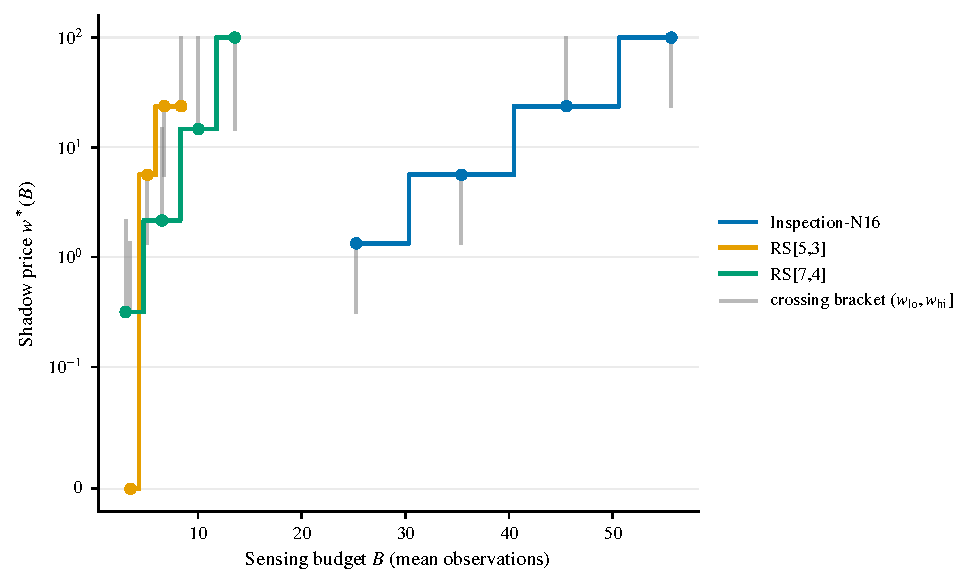
\includegraphics[width=0.85\textwidth]{figures/price_staircase_interleaved.pdf}
\caption{Shadow-price staircases $w^*(B)$ on three interleaved (non-observe-then-commit) settings, RockSample[5,3], RockSample[7,4], and Inspection-$N{=}16$, with crossing brackets marked. The underlying usage curves $U(w)$ are monotone at every sampled grid point on RockSample[7,4] and Inspection-$N{=}16$, while RockSample[5,3] dips once near $w{=}0.316$ before rising (see text).}
\label{fig:interleaved}
\Description{A single step plot of shadow price against sensing budget, with a logarithmic vertical axis running from 0 to 100. Three colored staircases. All three staircases rise from left to right without any downward step. The orange RockSample[5,3] staircase climbs from a price of 0 at a budget of about 3.5 to a price of about 24 by a budget of about 6.7, the green RockSample[7,4] staircase climbs from a price of about 0.3 at a budget of about 3 to a price of 100 at a budget of about 13.5, and the blue Inspection staircase sits farthest right, climbing from a price of about 1.3 at a budget of about 25 to a price of 100 at a budget of about 56. Gray vertical bars mark the crossing bracket at each step point.}
\end{figure}

\subsection{Supporting: shadow-price staircases}
\label{sec:stairs}

Figure~\ref{fig:stairs} reports $w^*(B)$ over identifiable budgets inside $[U_{\min}, U_{\max}]$ for Tiger, Diagnosis, Bandit, Tileworld-$6{\times}6$, and Inspection-$N{=}8$. Tiger, Diagnosis, and Inspection are exactly nondecreasing at every sampled grid point. Bandit and Tileworld show local non-monotonicity from discrete policy switches (the count-usage gap identified in Proposition~\ref{prop:pi2}'s scope note), so we report brackets and standard errors rather than singleton prices. Tiger's price is weakly identified, consistent with Table~\ref{tab:collapse-breadth}. Instrumental listening already saturates most of the usage range at $w{=}0$.

\begin{figure}[t]
\centering
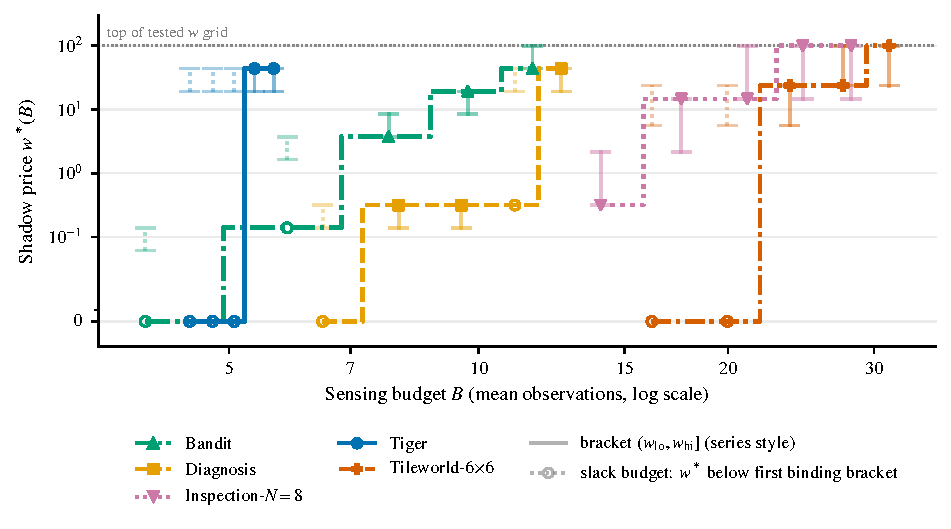
\includegraphics[width=0.85\textwidth]{figures/price_shadow_curves.pdf}
\caption{Operational shadow-price staircases with vertical crossing brackets, observe-then-commit and inspection domains.}
\label{fig:stairs}
\Description{A single plot of shadow price against sensing budget on a logarithmic vertical axis, with five colored staircase curves and gray vertical bracket bars. The vermillion Tiger staircase rises almost vertically near a budget of about 5.5. The blue Bandit and orange Diagnosis staircases climb between budgets of roughly 4 and 13. The green Inspection and pink Tileworld staircases climb between roughly 14 and 31. Tiger, Bandit, and Diagnosis step upward from zero to a top price of about 44, while Inspection and Tileworld reach 100, some with locally uneven step placement.}
\end{figure}

\subsection{A near-optimal offline reference: SARSOP}
\label{sec:sarsop}

The camera-ready replies to the workshop version promised a near-optimal offline baseline. We retire that debt here. We build the original APPL C++ SARSOP toolkit \citep{kurniawati2008} from source (Appendix~\ref{app:sarsop_build}) and export the three core observe-then-commit benchmarks to the Cassandra \texttt{.pomdp} format generically from the same generative model the agents already use, solve to precision $10^{-3}$ (under one second per environment at $\gamma{=}0.999$), and evaluate the resulting alpha-vector policy in-simulator through the same episode runner used for the other observe-then-commit agents, so the agents compared in Table~\ref{tab:sarsop} share mechanics and metrics exactly. Table~\ref{tab:sarsop} reports the full protocol ($5$ seeds $\times$ $500$ episodes).

\begin{table}[t]
\centering
\caption{SARSOP near-optimal reference vs.\ EFE ($w{=}1$) on the three core OTC environments (mean $\pm$ SE reward, mean usage $\pm$ SE in observation count, $\gamma{=}0.999$).}
\label{tab:sarsop}
%% Numbers in this table are produced by experiments/run_sarsop_baseline.py
\small
\begin{tabular}{lcccc}
\toprule
Environment & SARSOP reward & EFE reward & SARSOP usage & EFE usage \\
\midrule
Tiger & $5.061 \pm 0.158$ & $5.061 \pm 0.158$ & $4.323 \pm 0.045$ & $4.323 \pm 0.045$ \\
Diagnosis & $-1.452 \pm 0.336$ & $-1.217 \pm 0.184$ & $9.68 \pm 0.12$ & $9.73 \pm 0.13$ \\
Bandit & $6.280 \pm 0.134$ & $6.261 \pm 0.112$ & $5.16 \pm 0.09$ & $5.09 \pm 0.07$ \\
\bottomrule
\end{tabular}
\end{table}

On Tiger, SARSOP and EFE select identical actions on every episode. With a single observation action the near-optimal policy and the EFE policy coincide exactly. On Diagnosis and Bandit the two show no statistically significant reward difference at our sample sizes, with the Diagnosis means differing by about $0.6$ SE, and their usage differs by less than $0.1$ observations (Table~\ref{tab:sarsop}, Diagnosis $9.68 \pm 0.12$ against $9.73 \pm 0.13$, Bandit $5.16 \pm 0.09$ against $5.09 \pm 0.07$).

We formalize this with a predeclared-margin two one-sided tests (TOST) procedure \citep{schuirmann1987}. The margin was fixed before inspecting these samples at the cost of one sensing action in each environment, which is $\pm 1.0$ reward for Tiger and Diagnosis and $\pm 0.5$ for Bandit. It is an operational margin for this domain, not a universal equivalence standard. The test is an unpaired Welch $t$-test on per-seed means ($n{=}5$ seeds, $500$ episodes per seed) rather than on pooled episode-level values, so degrees of freedom reflect independent seeds. We do not pair by seed index even though EFE and SARSOP share a nominal seed list. Once the two policies diverge on an episode they consume the environment's random draws in different orders, so a shared seed label does not make the trajectories correlated, and pairing would understate the variance. All three environments reject both one-sided nulls at $\alpha{=}0.05$ (Tiger $p{=}0.0010$, Diagnosis $p{=}0.0458$, Bandit $p{=}0.0130$), the $90\%$ CI of each mean difference lies entirely inside the margin (Tiger $[-0.41,+0.41]$, Diagnosis $[-0.51,+0.98]$, Bandit $[-0.35,+0.31]$), and the three tests survive Holm--Bonferroni correction as a family. EFE at the canonical weight is therefore statistically equivalent to the SARSOP reference within the predeclared margin on this suite (\texttt{results\_tost\_sarsop.csv}).

Five seeds is thin. We reran the identical procedure at $n{=}20$ seeds, fixed before running rather than added post hoc, reusing the same SARSOP policies (\texttt{results\_tost\_sarsop\_n20\_robustness.csv}). All three environments remain equivalent, $p_{\mathrm{TOST}}$ tightens by roughly six, five, and eight orders of magnitude (Tiger $4.5{\times}10^{-10}$, Diagnosis $6.8{\times}10^{-7}$, Bandit $6.0{\times}10^{-11}$), and the intervals narrow accordingly, with Tiger's $90\%$ CI shrinking from $[-0.41,+0.41]$ to $[-0.21,+0.21]$.

Two negative results belong here. Inverting the offline usage curve to match SARSOP's usage exactly, rather than comparing at $w{=}1$, is ill-posed on Tiger because the curve is flat (Table~\ref{tab:collapse-breadth}), forcing a bracket as wide as $w \in (19.3, 43.9]$ to nominally match a target the curve cannot discriminate. We also considered POMCPOW \citep{sunberg2018} and declined it, because it exists to handle continuous state, action, and observation spaces via progressive widening, and every benchmark here is a discrete POMDP, with a near-optimal SARSOP reference on the three core observe-then-commit environments, and discrete POMCP (Appendix~\ref{app:pomcp}) already in hand on Tiger, Diagnosis, Bandit, Tileworld, and RockSample.

\subsection{A near-optimal constrained-POMDP reference}
\label{sec:cpomdp}

A natural objection to the single-price family is that no exact constrained-POMDP reference bounds it from above. We provide a near-optimal one for the three environments where SARSOP already serves as our near-optimal reference (Tiger, Diagnosis, Bandit, Section~\ref{sec:sarsop}), by extending the same SARSOP export with a literal per-unit usage penalty in the reward model. Each observation action's reward becomes $-(\text{cost}_j + \lambda)$ for $\lambda \ge 0$, so solving the resulting POMDP to SARSOP's precision ($10^{-3}$) gives, for that $\lambda$, a near-optimal solution to $\max_\pi \mathbb{E}_\pi[R] - \lambda\,\mathbb{E}_\pi[U]$ over the full space of POMDP policies (not the additive Planning+IG family). The reference is near-optimal rather than certified exact, because SARSOP is a point-based approximate solver and the reported reward and usage are themselves Monte Carlo estimates from simulated episodes, not closed-form quantities. For a finite discounted constrained MDP, strong Lagrangian duality holds \citep{altman1999}. That result covers finite state spaces, and the belief MDP here is continuous, so we do not assume a zero duality gap carries over. The swept points are supported points of the achievable region in any case, so they bound the frontier from below, and any duality gap makes the reference conservative rather than optimistic about what is achievable. Conservative here refers to frontier achievability alone. For the optimality comparison the direction reverses, since a reference that undershoots the constrained optimum makes our agents look closer to optimal than they are, so the measured gap to the reference is a lower bound on the true gap. Sweeping $\lambda$ over a log-spaced $12$-point grid ($\lambda \in [0, 100]$, $\gamma{=}0.999$, $5$ seeds $\times$ $300$ episodes per $\lambda$) traces an estimated upper concave envelope of the achievable $(\mathbb{E}[U], \mathbb{E}[R])$ region, sampled at these 12 supported points rather than continuously. A per-episode mixture of two adjacent swept policies approximates any intermediate budget, the same mixture argument used for the Planning+IG shadow price (Definition~\ref{def:pi3}), though the approximation inherits whatever slack the constituent near-optimal solutions carry. $\lambda{=}0$ recovers the ordinary reward-only SARSOP solve of Table~\ref{tab:sarsop} as a sanity check.

\begin{table}[h]
\centering
\caption{Estimated CPOMDP reference gap at the budget $B_{\mathrm{EFE}} = U(\text{EFE}, w{=}1)$, interpolated on the Lagrangian-sweep reference frontier. $R_{\mathrm{ref}}$ is the near-optimal SARSOP-Lagrangian reward at that usage (not a certified bound). The gap is $R_{\mathrm{ref}} - R_{\mathrm{EFE}}$. Planning+IG at the usage-matched weight $w^*$ (not $w{=}1$, but $w^*{=}0.00$, $0.45$, and $1.07$ for Tiger, Diagnosis, and Bandit respectively) attained reward bit-identical to EFE's on all three environments in this run (\texttt{results\_cpomdp\_baseline.csv}. \texttt{R\_PIG} matches \texttt{R\_EFE} to the precision stored), an empirical finding about this policy family and this suite, not a consequence of Proposition~\ref{prop:equivalence}, which is stated for $w{=}1$ specifically. A single gap column covers both.}
\label{tab:cpomdp}
%% Numbers in this table are produced by experiments/run_cpomdp_baseline.py
\small
\begin{tabular}{lccccc}
\toprule
Environment & $B_{\mathrm{EFE}}$ & $R_{\mathrm{ref}}$ & $R_{\mathrm{EFE}}$ & Gap & Gap \% \\
\midrule
Tiger & $4.32$ & $5.016$ & $5.016$ & $0.000$ & $0.00\%$ \\
Diagnosis & $9.82$ & $-1.297$ & $-1.224$ & $-0.073$ & $-5.65\%$ \\
Bandit & $5.10$ & $6.313$ & $6.320$ & $-0.007$ & $-0.11\%$ \\
\bottomrule
\end{tabular}
\end{table}

Table~\ref{tab:cpomdp} reports the comparison. The estimated gap is zero on Tiger and within one grid step of zero on Bandit ($-0.11\%$). Diagnosis shows a small negative gap ($-5.65\%$, i.e., the reference value is slightly below $R_{\mathrm{EFE}}$). Since a true optimum cannot lie below EFE's measured reward, a negative estimated gap indicates reference-frontier noise or resolution limits rather than a real violation. We attribute it to finite-sample noise at the usage ceiling combined with interpolation past the sampled grid. EFE's own measured usage ($9.824$) marginally exceeds the highest usage realized anywhere on the $12$-point $\lambda$ grid ($9.817$, at $\lambda{=}0.107$), so the reported $R_{\mathrm{ref}}$ is the clamped boundary value rather than an interpolation between two bracketing points, and both quantities are themselves $1{,}500$-episode Monte Carlo estimates with standard errors of comparable magnitude to the gap ($\pm 0.13$--$0.31$). A finer $\lambda$ grid near $0$ and more episodes per point would sharpen this estimate. We report the current resolution rather than tuning the grid to close the gap. Read together with Table~\ref{tab:sarsop}'s TOST result, the finding is that the calibrated Planning+IG family is not just close to the single reward-maximizing operating point, but empirically close to this near-optimal reference at the usage-matched budget $B_{\mathrm{EFE}}$, on this three-environment suite (\texttt{results\_cpomdp\_baseline.csv}, \texttt{results\_cpomdp\_frontier.csv}, \texttt{experiments/run\_cpomdp\_baseline.py}).

This provides a near-optimal constrained-POMDP reference for the discrete observe-then-commit suite. The optimality gap is estimated rather than certified, since it rests on an approximate solver evaluated by simulation. The scope is deliberately narrow. It does not extend to RockSample or Structural Inspection's larger factored state spaces, where SARSOP itself is no longer a practical solver at the sizes we study (Section~\ref{sec:budget_positioning} and Appendix~\ref{app:calibration}), so even an approximate optimality-gap estimate there remains future work.

\subsection{Distractor robustness: reward-irrelevant sensing}
\label{sec:distractor}

A recurring question about information-gain objectives is how they behave when uncertainty exists over state components that do not affect reward. We construct \texttt{DistractorDiagnosisEnv}, an $8$-joint-state Diagnosis variant ($4$ conditions $\times$ a binary nuisance bit, commit rewards depend only on the $4$-way condition) with one additional test that is informative only about the nuisance bit. Every observation model in the environment factors through exactly one of the two independent components, so the distractor test carries exactly zero information about the condition marginal. This is provable from the factorization, and it is unit-tested.

Sweeping Planning+IG over a log weight grid refined around the onset ($5$ seeds $\times$ $100$ episodes), the distractor fraction of total sensing usage is exactly $0$ for $w \le 3.5$, is $0.103 \pm 0.001$ at $w{=}4$, reaches $0.233 \pm 0.003$ by $w{=}5$, and saturates in the $0.330$--$0.332 \pm 0.004$--$0.005$ range for $w \ge 31.6$ (seed-level SE, Figure~\ref{fig:distractor}). The onset therefore lies in the bracket $(3.5, 4.0]$, where the agent buys its first distractor test. Ordinary information gain does not distinguish reward-relevant from reward-irrelevant uncertainty, so once the weight is large enough to make the distractor's nonzero (but task-useless) information gain worth its cost, Planning+IG spends budget on it. The sensing budget of Section~\ref{sec:budget} caps how much total sensing is bought but does not by itself redirect that spending toward reward-relevant tests. EFE at the canonical $w{=}1$ happens to stay at zero distractor fraction on this instance, but only because the onset bracket $(3.5, 4.0]$ lies above $1$ here, not because EFE is structurally immune to the effect. An instance with a lower onset would show EFE chasing the distractor too. A budget caps total spend but does not redirect it, because $I(b)$ is computed over the full joint belief rather than over the quantities the pending commit decision actually depends on. The repair is to score information gain on the reward-relevant marginal, $\tilde{I}_a(b) = D_{\mathrm{KL}}\!\big[Q(s_{\mathrm{rel}} \mid o, a) \,\|\, Q(s_{\mathrm{rel}} \mid a)\big]$, restricted to the state components $s_{\mathrm{rel}}$ the commit reward depends on.

Identifying $s_{\mathrm{rel}}$ turns out to need no information the agent does not already hold. Two states are reward-equivalent when every commit action pays the same in both, so no belief mass moved between them can change which commit action is optimal, and that partition is read directly off the commit reward matrix the agent is given (Section~\ref{sec:methodology}). We implement the variant that way, as a partition into reward-equivalence classes with information gain scored on the class marginal. Belief dynamics are untouched, since the continuation always propagates the full joint posterior and only the epistemic scoring term changes. On an environment where no two states are reward-equivalent the variant reduces exactly to ordinary information gain.

Sweeping both variants over the same refined weight grid makes the effect a paired curve rather than a single point (Figure~\ref{fig:distractor}). The relevance-weighted agent takes exactly zero distractor tests at every one of the sixteen swept weights, against $6.46$ tests and $33.2\%$ of total usage for ordinary information gain at $w{=}100$. It recovers the full reward cost of that spending, $-2.45$ to $-1.45$ at $w{=}4$, $-4.31$ to $-1.45$ at $w{=}5$ and $w{=}10$, and $-10.48 \pm 0.11$ to $-3.64 \pm 0.36$ at $w{=}100$ (seed-level SE). Accuracy is never the price, with success rates bit-identical through $w{=}31.6$ and nominally higher for the variant at $w{=}100$ ($99.2\%$ against $98.4\%$, not significant). Seed-level Welch tests with Holm--Bonferroni correction over the weight-by-metric family confirm the usage and distractor-count differences at every weight past onset, and the reward difference at $w{=}31.6$ and $w{=}100$ ($p{=}1.2{\times}10^{-5}$ and $1.5{\times}10^{-5}$).

The boundary of what this fixes matters as much as the fix. At the two largest weights the relevance-weighted agent still runs $13.16$ task tests where a moderate weight runs $9.77$, so it has stopped buying reward-irrelevant information and has not stopped over-buying reward-relevant information. The two instruments are complementary rather than redundant. A sensing budget caps how much information is bought, and relevance weighting decides what it is bought about. Neither substitutes for the other, and this environment needs both.

\begin{figure}[t]
\centering
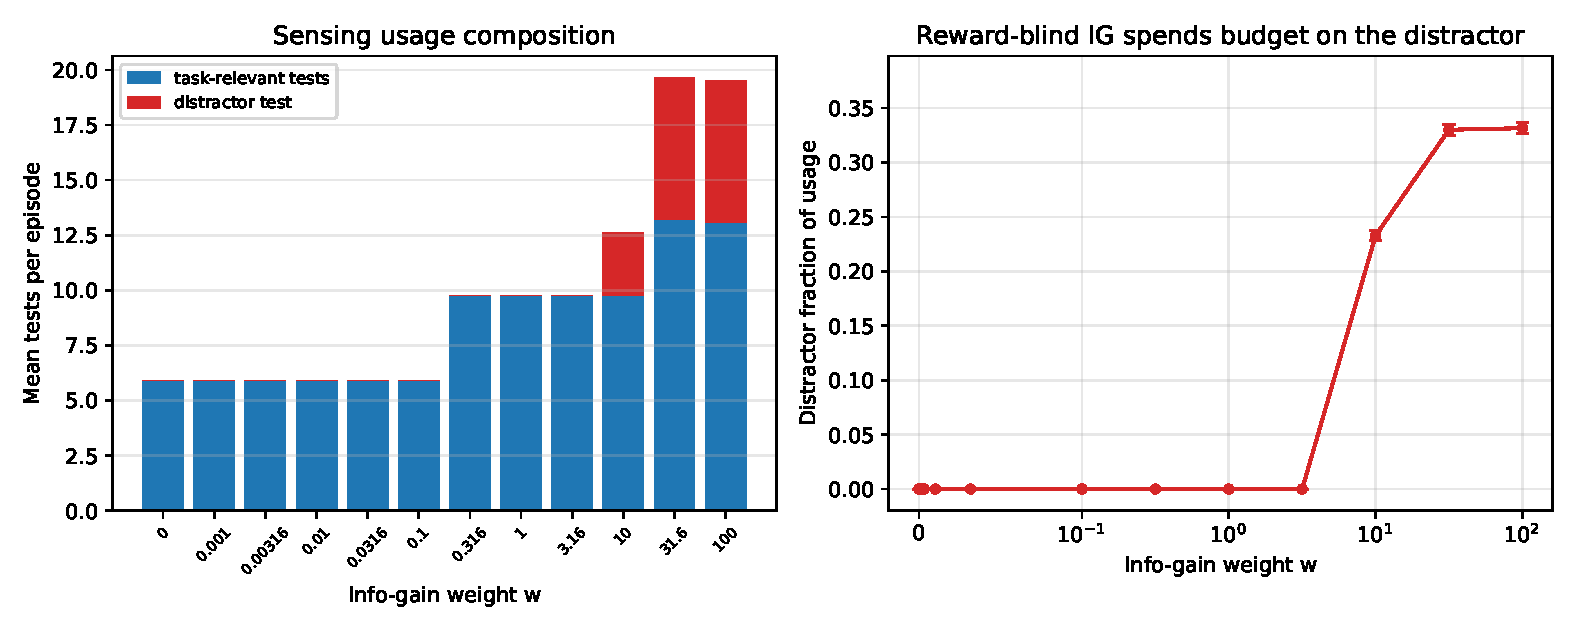
\includegraphics[width=0.85\textwidth]{figures/distractor_composition.pdf}
\caption{Reward-irrelevant sensing on \texttt{DistractorDiagnosisEnv}. The left panel decomposes ordinary Planning+IG's usage into task-relevant and distractor tests as $w$ grows. Distractor spend is zero below the onset bracket $(3.5, 4.0]$ and saturates at roughly a third of total usage. The right panel plots the distractor fraction for ordinary information gain against the reward-relevance-weighted variant on the same grid. The weighted variant is flat at exactly zero everywhere. Error bars are seed-level SE over 5 seeds.}
\label{fig:distractor}
\Description{Two panels. The left panel is a stacked bar chart of mean tests per episode across sixteen weight values, with blue task-relevant segments stepping from about 6 up to about 13 and a vermillion distractor segment that is absent at small weights, first appears at a weight of 4, and grows the stack to about 20 tests at the two largest weights. The right panel plots two curves of distractor fraction against weight on a log axis. The vermillion curve for ordinary information gain is flat at zero up to a weight of 3.5, rises steeply from 0.10 at weight 4 through 0.23 at weight 5, and levels off near 0.33. The green curve for the reward-relevance-weighted variant lies flat on zero across the entire range.}
\end{figure}

We also checked whether information-directed sampling (IDS) \citep{russo2014}, which is explicitly reward-aware through its information-ratio numerator, is immune. It is not, for an implementation reason worth reporting exactly. IDS's \texttt{info\_astar} term (information about the optimal commit) is correctly zero for the distractor action, but the implementation falls back to a raw state-entropy term (\texttt{info\_state}) whenever \texttt{info\_astar} is at or near zero, and that fallback lets the distractor's genuine nuisance-bit informativeness through. Instrumented directly, IDS's distractor fraction is $0.305 \pm 0.005$ (seed-level SE), close to but measurably below Planning+IG's saturated $0.330$--$0.332 \pm 0.004$--$0.005$ at large $w$ (roughly a $3$-SE gap, so not a clean tie, though both sit well above zero). This is not evidence that reward-aware information measures are useless against distractors in general. It is evidence that a specific, common implementation pattern (falling back to unconditional entropy reduction when the reward-conditional information measure vanishes) reintroduces exactly the reward-blindness the reward-aware measure was meant to avoid. Neither ordinary information gain nor the in-repo IDS adaptation is therefore a clean immune baseline against reward-irrelevant sensing on this benchmark. The reward-relevance-weighted variant above is the clean case, and the contrast is instructive. It has no raw-entropy fallback to reintroduce reward-blindness, because it does not compute a reward-conditional quantity that can vanish and then need replacing. It scores ordinary information gain on a coarsened state space, so a test that is uninformative about the reward-equivalence classes earns exactly zero rather than a small positive number that a fallback then rescues. Appendix~\ref{app:ids} reports the IDS baseline in full on the observe-then-commit environments.

\subsection{The $w^*$ atlas}
\label{sec:w_atlas}

Table~\ref{tab:w-atlas} (Appendix~\ref{app:w_atlas}) collects the implicit EFE budget $B_{\mathrm{EFE}} = U(w{=}1)$ and two canonical-budget crossing brackets for the eight benchmark instances whose usage curves we estimate, aggregating those curves across Sections~\ref{sec:results} and~\ref{sec:budget_experiments}. This is an atlas of measured operating points, not a predictive meta-model relating $B_{\mathrm{EFE}}$ to environment parameters (reward scale, state count, horizon). No such closed form is claimed, and the atlas should not be read as one.

\section{Discussion}
\label{sec:discussion}

\paragraph{The information weight as an operational shadow price.}
Every claim below about $w{=}1$ being an untuned default is conditional on one reward convention shared across every comparison in this paper. That conditioning is the correct framing rather than a caveat. Information gain is measured in bits while task reward is measured in whatever units the designer chose, so the pragmatic-epistemic exchange rate $w$ is necessarily convention-dependent, and Proposition~\ref{prop:pi1} proves that dependence is exact and predictable rather than merely bounded for the implemented agent. This lets us replace ``what should $w$ be'' with ``how much sensing can we afford,'' a question with a physically meaningful answer that a designer can state without knowing anything about information theory. The answer is a budget $B$ in observation count or cost. Section~\ref{sec:budget_experiments} shows the resulting operational shadow price $w^*(B)$ is computable offline from a usage curve and convergent under stationarity via dual descent (Proposition~\ref{prop:pi5}), with re-adaptation through a reward-scale shift demonstrated empirically (Section~\ref{sec:dual_multiseed}). At the specific budget $B_{\mathrm{EFE}} = U(w{=}1)$ it recovers EFE's canonical weight as the special case that buys whatever sensing the ambient reward scale happens to imply (Section~\ref{sec:pi1}). The distractor-robustness result (Section~\ref{sec:distractor}) marks the boundary of what a budget alone can do, and supplies the missing half. A sensing budget caps how much total information an agent buys, and neither ordinary information gain nor the reward-aware IDS baseline we tested redirects that budget away from reward-irrelevant uncertainty on its own. Scoring information gain on the reward-relevance partition does redirect it, to exactly zero reward-irrelevant spend at every swept weight, using nothing the agent does not already hold. Price and relevance are complementary instruments. The budget decides how much information is bought, the partition decides what it is bought about.

\paragraph{When does EFE-as-$\rho$ help?}
The per-decision value-of-information audit trail (Appendix~\ref{app:audit}) exposes the decomposition behind these decisions, and Appendix~\ref{app:calibration} scores the terminal belief itself rather than the decision it produces. EFE's advantage requires (1)~multiple observation actions with differential informativeness and (2)~sufficient planning horizon for recursive EFE to propagate epistemic value. When condition (1) fails, as on Tiger with its single listen action, reward-only planning matches EFE. The Tileworld adds a third axis. As the state space grows, the reward signal becomes too diffuse to guide scan selection. The separation is a threshold rather than a steady growth, absent within one standard error of the difference at $4{\times}4$ and $6{\times}6$ and opening at $8{\times}8$, where Planning collapses (Figure~\ref{fig:tw_scaling}). Within-episode dynamics (Appendix~\ref{app:foraging}) show the mechanism. EFE concentrates belief via partition-based narrowing and commits once the value of committing exceeds the value of observing, a crossover that emerges automatically from $w{=}1$ without tuning (Figure~\ref{fig:traj}, Appendix~\ref{app:efe_trajectory}).

\paragraph{The information-unit weight and why it works.}
EFE does not eliminate the exploration--exploitation weight. It supplies a derived relative coefficient in information units under a fixed reward convention. The Pareto analysis (Figure~\ref{fig:pareto}) shows this weight sits inside the reward-maximizing tied bracket on three of the five swept environments, while the success-maximizing $w^*_{\text{succ}}$ used for Planning+IG in the main tables lies at $10$--$50$. The gap between $w^*_{\text{ret}}$ and $w^*_{\text{succ}}$ has practical implications. $w{=}1$ targets expected reward, not success probability. In safety-critical settings where near-certain accuracy is required, a higher weight may be appropriate, though such weights must still be tuned per-environment. EFE provides a principled starting point rather than a scale-free automatic calibration. On Tiger and Diagnosis, moving to the success-tuned $w{=}50$ buys at most $1.8$pp of accuracy while costing $1.07$ and $2.41$ reward, and the reward stays flat between $w{=}1$ and that point. Bandit trades more evenly, gaining $9.8$pp success for $0.41$ reward at $w{=}5$, and Tileworld rises to an interior reward optimum at $w{=}20$ before falling. Moreover, adding planning depth to a weighted IG bonus amplifies the weight's effect, making the tuning problem harder with depth. At $w{=}100$ on Bandit under the canonical 5-seed protocol, Planning+IG at $H{=}2$ takes $12.36$ inspections against myopic Info Gain's $11.50$ (seed-level Welch $p{=}0.003$, \url{experiments/run_bandit_w100_depth_comparison.py}). Identifying pragmatic value with task reward chooses $P(o|C) \propto \exp(\beta R)$ with $\beta{=}1$ per reward unit, so keeping $w$ fixed while rescaling rewards by $k$ rescales the effective weight by $1/k$. The claim is exact under log scoring rules \citep{bernardo1979}. Our implementation uses bits ($\mathrm{base}{=}2$). Nat/bit conversion multiplies $w$ by $\ln 2 \approx 0.69$. On Tiger and Diagnosis the conversion stays inside the wide reward-tied bracket and changes no qualitative conclusion, though the sweep does not evaluate $0.69$ itself. On Bandit it lands just below the $[1,2]$ bracket. On Testbed it changes which claims hold, and on Tileworld both conventions are Pareto-dominated by $w{=}20$. Section~\ref{sec:pareto} reports the measured sweeps behind each exception.

The information-unit weight's advantage requires $\gamma \geq 0.99$ on multi-observation environments. Our discount-sensitivity analysis (Appendix~\ref{app:discount}, 5 seeds) reveals a sharp transition. On Diagnosis ($N{=}4$), EFE's success advantage over Planning is $+8.6$pp at $\gamma{=}1.0$ and $+7.9$pp at $\gamma{=}0.99$ (both seed-level Welch $p<10^{-4}$), but is not statistically significant at $\gamma{=}0.95$ or $\gamma{=}0.90$ (diff $\approx 0.04$pp, $p{=}0.96$ at both). The mechanism is that discounting truncates the effective planning horizon below the number of observations needed for confident diagnosis, erasing EFE's advantage. On Tiger (single observation), EFE and Planning differ significantly only at the heaviest discounting tested ($\gamma{=}0.90$, $+2.7$pp, $p<10^{-3}$) and are numerically identical at $\gamma \geq 0.95$. This is a meaningful practical limitation. Applications with high time pressure or non-stationary environments that mandate heavy discounting will not benefit from EFE's epistemic drive.

\paragraph{Zero-shot weight transfer.}
The tuning problem is not merely inconvenient. Transfer depends on the tuning criterion. Table~\ref{tab:transfer} evaluates $w{=}1$, reward-tuned weights $w^*_{\mathrm{ret}}$, and success-tuned weights $w^*_{\mathrm{succ}}$ across environments. Success-tuned transfer harms reward at the top of the grid. $w^*_{\mathrm{succ}}{=}50$, the class-correct success-tuned weight for both Tiger and Diagnosis, yields $+4.25$ on Tiger and $-0.38$ on Testbed versus $w{=}1$ at $+5.33$ and $+0.37$. Reward-tuned moderate weights ($w\in\{0.5,1\}$) transfer well within the shared reward scale, and $w{=}1$ is tied for best on Tiger and Diagnosis (alongside $w{=}0.5$, Testbed's $w^*_{\mathrm{succ}}{=}10$, and Bandit's $w^*_{\mathrm{succ}}{=}20$, since both reward landscapes are flat enough at moderate weights that the ties collapse together) and remains best outright on Bandit without search. The honest conclusion is that moderate weights transfer robustly under a shared reward convention whatever their provenance, while success-tuned weights overfit once pushed to $w{=}50$, the top of the tested grid. In that moderate band, $w{=}1$ is the variational default, not a scale-free optimum.

\begin{table}[ht]
\centering
\caption{Zero-shot weight transfer (500 episodes $\times$ 5 seeds, reward reported as mean $\pm$ seed-level SE, \texttt{results\_transfer.csv}). Rows include $w{=}1$, reward-tuned weights ($w^*_{\mathrm{ret}}$), and success-tuned weights ($w^*_{\mathrm{succ}}$), the Planning+IG-class values recorded in \texttt{results\_supplementary\_tuned\_weights.csv}, matching the evaluated agent class. Success-tuned transfer harms reward at the top of the grid, while moderate weights transfer well. Bold. Best reward per column (Tiger and Diagnosis show a four-way tie among $w \in \{0.5, 1, 10, 20\}$, bit-identical under the fixed pipeline, not merely within SE).}
\label{tab:transfer}
%% Numbers in this table are produced by experiments/run_transfer.py
\begin{small}
\begin{tabular}{lcccc}
\toprule
Weight & Tiger & Diagnosis & Bandit & Testbed \\
\midrule
$w{=}0.5$ ($w^*_{\mathrm{ret}}$ Diag./Testbed) & $\mathbf{+5.33 \pm 0.26}$ & $\mathbf{-1.26 \pm 0.34}$ & $+6.05 \pm 0.11$ & $\mathbf{+0.48 \pm 0.02}$ \\
$w{=}1$ (EFE / $w^*_{\mathrm{ret}}$ Tiger/Bandit) & $\mathbf{+5.33 \pm 0.26}$ & $\mathbf{-1.26 \pm 0.34}$ & $\mathbf{+6.24 \pm 0.09}$ & $+0.37 \pm 0.01$ \\
$w{=}10$ ($w^*_{\mathrm{succ}}$ Testbed) & $\mathbf{+5.33 \pm 0.26}$ & $\mathbf{-1.26 \pm 0.34}$ & $+5.25 \pm 0.06$ & $+0.01 \pm 0.01$ \\
$w{=}20$ ($w^*_{\mathrm{succ}}$ Bandit) & $\mathbf{+5.33 \pm 0.26}$ & $\mathbf{-1.26 \pm 0.34}$ & $+5.05 \pm 0.07$ & $-0.18 \pm 0.01$ \\
$w{=}50$ ($w^*_{\mathrm{succ}}$ Tiger/Diag.) & $+4.25 \pm 0.08$ & $-3.68 \pm 0.14$ & $+4.23 \pm 0.06$ & $-0.38 \pm 0.01$ \\
\bottomrule
\end{tabular}
\end{small}
\end{table}

\paragraph{When is $w{=}1$ near-optimal?}
Proposition~\ref{prop:nearopt} formalizes lower and upper thresholds for the two-state case. $w^*_{\mathrm{lo}}$ depends on reward asymmetry $\alpha = |R^-|/R^+$, informativeness $\eta = I_{\max}/c$, and accuracy $p$, while $w^*_{\mathrm{hi}}$ bounds over-observation at the post-first-observation belief. Table~\ref{tab:alpha_eta} is consistent with this prediction on the genuinely two-state rows and, more heuristically, on the two-state-reduced rows (Bandit omitted as multi-arm). High-asymmetry environments ($\alpha \geq 5$, namely Tiger, Diagnosis, and Tileworld) have $w^*_{\mathrm{lo}} \ll 0$ and $w^*_{\mathrm{hi}} \approx 7$--$8$, so $w{=}1$ is interior. Testbed places $w{=}1$ near the upper bound, consistent with over-exploration.

To assess whether the $H{=}1$ analysis extends to multi-step planning, we conducted a Monte Carlo study over 100 randomly generated two-state environments (sampling $\alpha \in [1, 50]$, $p \in [0.55, 0.95]$, cost $\in [0.1, 5]$). For each environment and $H \in \{1, 2, 3\}$, we compute the reward-optimal $w^*$ by grid search and classify $w{=}1$ as near-optimal when the reward gap from $w^*$ is within $\max(5\%, 0.5)$ of the best reward (Figure~\ref{fig:nearopt_horizon}). The near-optimality rate increases from 30\% at $H{=}1$ to 58\% at $H{=}2$ and 79\% at $H{=}3$, confirming that multi-step planning amplifies the value of observation and expands the region where $w{=}1$ is near-optimal. High-asymmetry environments ($\alpha \geq 10$) follow the same trend, rising from 26\% to 53\% to 79\%. The complement is the more useful number for a practitioner and we state it directly. $w{=}1$ fails this near-optimality test in about $21\%$ of the random family even at $H{=}3$, and in $70\%$ of it at $H{=}1$. The criterion is also lenient by construction, counting $w{=}1$ as near-optimal whenever it is within $\max(5\%, 0.5)$ of the best achievable reward, so the absolute floor of $0.5$ reward units does most of the work on environments whose reward range is small. This is qualitatively consistent with the Bandit result. Bandit's reward asymmetry is low relative to the high-asymmetry environments above (correct-arm reward $+10$ vs.\ small-reward-arm $+1$, not the two-state $\alpha{=}|R^-|/R^+$ ratio this section's formula assumes, so we do not report a numeric $\alpha$ for it), so the $H{=}1$ analysis predicts only marginal sufficiency, yet multi-step EFE at $H{=}2$ achieves $86.9\%$ success (Table~\ref{tab:main}).

Many real-world decision problems have $\alpha \gg 1$. In medical diagnosis, fault detection, and security screening, a missed condition costs far more than another test. This is the regime where the interval analysis is most favorable to $w{=}1$, and the multi-step study shows the near-optimality basin widening with planning depth ($79\%$ of $\alpha \ge 10$ environments pass at $H{=}3$, up from $26\%$ at $H{=}1$). The practical consequence is calibrated accordingly. In these domains the information-unit weight is a strong untuned starting default under the shared reward convention, not a guarantee of near-optimality, and the budgeted machinery of Section~\ref{sec:budget} is the recourse when the default's induced sensing does not match what the application can afford.

\paragraph{Robustness to model misspecification.}
Our main results assume exact knowledge of the generative model. Appendix~\ref{app:misspec} investigates robustness when the agent's believed observation accuracy differs from the true value, over mismatches from $-0.15$ to $+0.10$. On Tiger, success stays within $2.7$pp of the calibrated $99.6\%$ at every tested level, and EFE and Planning respond identically to every tested mismatch (Table~\ref{tab:misspec-tiger}), so there is no measurable EFE-specific buffering effect on this environment. On Diagnosis, degradation is larger but graceful, and both agents' behavior steps between two levels rather than degrading smoothly with the mismatch magnitude. Overestimating sensor accuracy (positive mismatch) is more harmful than underestimating it, because the agent commits prematurely on insufficient evidence.

\paragraph{Approximate planning with MCTS-EFE.}
At each depth the tree branches over $K$ observation actions and then, per action, over its $|\mathcal{O}|$ observation outcomes, so the exact tree search cost is $\mathcal{O}((K \cdot |\mathcal{O}|)^H)$, limiting practical horizons to $H{=}2$--$3$ with $K \geq 3$. To push beyond this, we implement MCTS with EFE as a leaf heuristic. The tree policy uses UCB1 with observation-outcome enumeration, and leaf nodes are evaluated via greedy EFE rollouts. On Tiger at $H{=}10$, MCTS-EFE with 500 simulations achieves $97.7\% \pm 0.5$pp success ($23$--$28$ ms per episode, \texttt{results\_mcts\_efe.csv}), compared to $88.8\% \pm 0.2$pp for POMCP at the same simulation count ($15$--$19$ ms per episode, seed-level SE, seed-level Welch $p{=}5.2{\times}10^{-6}$, the comparison is simulation-matched, not compute-matched, since MCTS-EFE's leaf evaluations are more expensive per simulation). In this configuration, EFE's closed-form information valuation provides a stronger leaf heuristic than semi-informed rollouts. We say ``in this configuration'' advisedly. The observe-then-commit POMCP runs with a single untuned UCB1 exploration constant per battery, $10.0$ in the baseline comparison of Appendix~\ref{app:pomcp} and $5.0$ in the MCTS-EFE comparison reported here, so we cannot separate the contribution of directed observation selection from that of solver configuration there, and a per-environment exploration sweep could narrow this gap. The RockSample POMCP, by contrast, was tuned over a predeclared grid on disjoint seeds (Appendix~\ref{app:rocksample}). The comparison avoids a pure-random-rollout strawman. Our implementation already uses belief-optimal commits (not purely random rollouts). Observations are sampled uniformly, but the rollout terminates with the commit action maximizing expected reward under the Bayesian-updated belief (Appendix~\ref{app:pomcp}). Directed observation selection appears to be what drives the remaining performance gap, though it is not fully separable from solver configuration. EFE chooses which test to run based on information gain, while POMCP samples tests uniformly. The claim is not that EFE-based planning exceeds state-of-the-art POMDP solvers, but that the EFE leaf heuristic provides a principled, zero-tuning alternative to heuristic rollout design. POMCP with fully informed rollouts (e.g., using domain knowledge or a learned value function for observation selection) would narrow the gap further.

The approach also scales to multiple observation actions. For single-observation environments, the observation-outcome enumeration (2 outcomes per action) keeps expansion costs low. On Diagnosis ($N{=}4$, $K{=}2$ tests), MCTS-EFE at $H{=}5$ achieves $94.2\% \pm 0.5$pp success compared to POMCP's $68.7\% \pm 1.8$pp at the same simulation count (200 simulations, seed-level SE, seed-level Welch $p{=}7.2{\times}10^{-5}$, \texttt{results\_mcts\_efe.csv}), demonstrating that EFE scales to multi-observation environments. To exercise the approach on a larger multi-observation environment, we evaluate on Tileworld $6{\times}6$ ($|S|{=}36$, $K{=}6$ scans). MCTS-EFE saturates at $95.4\% \pm 0.6$pp success across both simulation budgets tested (200 and 500, seed-level SE), well above Exact-EFE's $71.9\% \pm 1.5$pp, but at a reward cost ($-25.02$ vs.\ Exact-EFE's $-21.62$) from scanning substantially more (32.3 vs.\ 14.8 observations on average). MCTS's sampled rollouts do not value information as precisely as the exact recursion, so it trades reward for a large success-rate gain by scanning more thoroughly. On Tiger and Diagnosis the trade runs the other way, with MCTS-EFE close to Exact-EFE on success and below it on reward as well ($+3.74$ against $+5.65$ on Tiger, $-3.26$ against $-1.44$ on Diagnosis). POMCP collapses on this larger observation menu regardless of simulation budget ($10.7\% \pm 1.1$pp at 200 simulations, $5.6\% \pm 1.1$pp at 500, seed-level SE), so MCTS-EFE's $85$--$90$pp success-rate gap over POMCP (seed-level Welch $p<10^{-9}$ at both budgets) indicates that directed observation selection remains essential at this scale even though the specific reward/success trade-off MCTS-EFE strikes here differs from the smaller environments. Semi-informed rollouts still cannot identify which of the 6 scans to perform. For larger observation spaces, more efficient tree policies, such as progressive widening or double progressive widening \citep{benchetrit2025}, would further improve scalability. We leave this to future work.

\paragraph{When to use EFE-as-$\rho$, in summary.}
Our analysis identifies the following conditions favoring EFE over tuned alternatives:
\begin{itemize}[leftmargin=1.5em,itemsep=1pt,topsep=2pt]
\item[] The three numeric thresholds below ($\alpha$, $H$, $\gamma$) are estimated from this paper's benchmark suite, not established regime boundaries. Read them as starting heuristics whose evidence is the experiments reported here.
\item Reward asymmetry $\alpha \geq 5$. The penalty for a wrong commit far exceeds the observation cost, placing $w{=}1$ well inside Proposition~\ref{prop:nearopt}'s $H{=}2$ near-optimality interval on our suite (Proposition~\ref{prop:nearopt}). The random-environment study tempers this into a favorable-regime heuristic rather than a guarantee ($79\%$ of $\alpha \ge 10$ samples pass at $H{=}3$, Appendix~\ref{app:nearopt_horizon}).
\item Multiple observation actions. EFE's joint pragmatic--epistemic objective selects which information to gather, producing gains over reward-only planning even at matched horizon.
\item Enough slack between greedy and information-optimal behavior that the agent's search can actually reach it. State-space size alone does not predict this. As the reward signal diffuses, directed information gathering becomes essential. On the Tileworld sweep the separation is a threshold rather than a steady growth. EFE ties Planning within one standard error of the difference at $4{\times}4$ and $6{\times}6$, then separates at $8{\times}8$, where Planning collapses ($69.4\%$ against $1.4\%$ success, Figure~\ref{fig:tw_scaling}). This is not a general scaling law in the other direction either. Diagnosis at $N{=}16$ under the $H{=}2$ scaling protocol shows no consistent EFE--Planning gap (Appendix~\ref{app:scaling}). The advantage vanishes on RockSample[11,11] ($|S|{=}2{,}048$, Section~\ref{sec:rocksample}) and, on Structural Inspection ($|S|$ up to $65{,}536$), the accuracy gap narrows, not grows, from $N{=}8$ to $N{=}16$. What predicts the advantage is how much slack separates greedy from information-optimal behavior, not $|S|$ per se.
\item Interleaved observe-act with preserved hidden state. When the hidden state does not change under observation and navigation actions (factored observation POMDPs, Table~\ref{tab:taxonomy}), the information-unit-weight equivalence holds and EFE directs both where to go and what to check (Tables~\ref{tab:rocksample},~\ref{tab:inspection}).
\item Cross-environment deployment. When the weight cannot be tuned per-task, how well a moderate weight transfers depends on the target environment. $w{=}1$ ties the transferred success-tuned $w{=}10$ and $w{=}20$ on Tiger and Diagnosis, where only $w{=}50$, the top of the tested grid, degrades, while on Bandit and Testbed every transferred success-tuned weight costs reward relative to $w{=}1$ (Table~\ref{tab:transfer}).
\item Planning horizon $H \geq 2$. Recursive EFE propagates epistemic value across steps. At $H{=}1$, it reduces to myopic IG with $w{=}1$.
\item Discounting $\gamma \geq 0.99$. Heavier discounting truncates the effective horizon below the number of observations needed for confident disambiguation, erasing EFE's advantage on multi-observation environments (Appendix~\ref{app:discount}). Like the other thresholds in this list, this one is read off two environments at one horizon each and should not be treated as a general boundary.
\end{itemize}
EFE is not recommended when $\alpha \approx 1$ (symmetric penalties), in navigation-style POMDPs where observations are tied to translation and a greedy mover already receives informative feedback (Table~\ref{tab:nav_scaling}), or when the model overestimates observation accuracy, the direction where measured degradation already appears at $+0.05$ mismatch (Appendix~\ref{app:misspec}).

\paragraph{Limitations and future work.}
The formal equivalence extends from observe-then-commit (Proposition~\ref{prop:equivalence}) to factored observation POMDPs (Proposition~\ref{prop:factored}), covering settings where observation actions preserve the hidden state. POMDPs where information-gathering actions change the hidden state (e.g., destructive testing) require the full coupling term $\Delta_T$ and are not covered. Extending the formal treatment to such settings remains future work. For slowly drifting hidden states (e.g., progressive disease), $\Delta_T$ is small but nonzero. The approximation error is governed by how far the transition kernel sits from the identity on the hidden state, not by its entropy. Example~\ref{ex:destructive} makes the distinction concrete, since its destructive test is deterministic and therefore has zero transition entropy while its coupling term is maximal. Characterizing the regime where the error remains acceptable is an open question.

On the practical side, scaling MCTS-EFE to multi-observation environments requires more efficient tree policies, as discussed above. The EFE agent assumes a known generative model. The misspecification analysis (Appendix~\ref{app:misspec}) shows graceful degradation with moderate model errors, but extending to full model learning (where AIF and BAMDPs converge) remains important future work. Navigation (Appendix~\ref{app:navigation}) shows that scale alone does not rescue epistemic planning when the observation model is proximity-based. NavMyopic leads nominally at all three grid sizes tested and significantly at $5{\times}5$, and no epistemic agent significantly beats it at any size (Appendix~\ref{app:navigation}). The practical contrast is with domains that offer explicit, choice-set observation actions (Diagnosis, Tileworld, RockSample), where EFE separates from reward-only planning once the search depth reaches the informative actions and greedy behavior has slack to lose. State-space size alone does not predict it. The separation is absent at Tileworld $4{\times}4$ and $6{\times}6$, absent at Diagnosis $N{=}16$, and absent at RockSample[11,11], and present at Tileworld $8{\times}8$, RS[5,3], RS[7,4], and RS[7,8]. On RockSample[11,11] the separation vanishes because no feasible search depth reaches the informative checks. The reductions here are exact while the numeric guidance is estimated from this suite, and the principled derivation of exploration weights could benefit safety-critical decision-making by reducing reliance on ad-hoc tuning.

\section{Conclusion}

We treat the weight on an information-gain utility as a price rather than a hyperparameter. Recasting $w$ as the operational shadow price of a sensing budget $B$ (Section~\ref{sec:budget}) turns a scale-invariance caveat into a theorem. The resulting policy family is exactly scale equivariant (Proposition~\ref{prop:pi1}), the shadow price is set-valued at usage gaps rather than falsely point-valued (Definition~\ref{def:pi3}), Proposition~\ref{prop:nearopt}'s closed-form onset thresholds are recovered as the first knot of the usage staircase (Corollary~\ref{cor:pi4}), and an online dual controller tracks the budget through a $\times 10$ reward rescale with disjoint-CI evidence that a reset-on-shift mechanism re-adapts roughly $2.65\times$ faster than decay alone (Section~\ref{sec:dual_multiseed}). An atlas of implicit budgets (Appendix~\ref{app:w_atlas}) reports where the eight benchmark instances with estimated usage curves actually sit on those curves. We also reported where the budgeted formulation does not help on its own. Ordinary information gain, and a common reward-aware baseline's raw-entropy fallback, both spend a sensing budget on reward-irrelevant uncertainty, and a budget caps that spending without redirecting it. Scoring information gain on the reward-equivalence partition of the state space redirects it completely, taking reward-irrelevant usage to zero at every swept weight and recovering the full reward it cost, while leaving over-spending on reward-relevant tests untouched (Section~\ref{sec:distractor}). Naive information gain can also misvalue an action outright once observation changes the hidden state (Example~\ref{ex:destructive}). The price of information, in this sense, is whatever weight the stated sensing budget requires, not a universally correct number.

What makes that price curve interpretable is a second result. The $\rho$-POMDP framework and active inference converge on the same mathematical object, a belief-dependent utility that adds information gain at weight $w{=}1$ to the reward signal under a fixed reward convention. EFE does not eliminate the exploration-exploitation trade-off. It replaces ad hoc bonus weights with a derived relative coefficient in information units, exact under log scoring rules \citep{bernardo1979} and empirically a robust untuned default, though not scale-invariant, and it doubles as the Planning+IG weight in Proposition~\ref{prop:equivalence}. Under that convention, the Pareto analysis places $w{=}1$ inside the reward-maximizing tied bracket on Tiger, Diagnosis, and Bandit, with further increases buying only marginal accuracy at substantial reward cost on Tiger and Diagnosis while Bandit trades more evenly ($+9.8$pp success for $0.41$ reward at $w{=}5$), but outside it on Testbed and Pareto-dominated by $w{=}20$ on Tileworld (Section~\ref{sec:pareto}). A near-optimal offline reference confirms, via a predeclared-margin TOST equivalence test, that this canonical weight is statistically equivalent to SARSOP on the three core observe-then-commit environments (Section~\ref{sec:sarsop}), and a near-optimal Lagrangian-sweep constrained-POMDP reference finds it close to Pareto-efficient against an estimated constrained-optimal frontier on the same three environments (Section~\ref{sec:cpomdp}). Safety-critical settings that demand near-certain accuracy may still prefer higher tuned weights, and a Monte Carlo study (Appendix~\ref{app:nearopt_horizon}) shows the near-optimality basin widens with planning horizon.

Proposition~\ref{prop:factored} carries the bridge beyond observe-then-commit into factored observation POMDPs, from RockSample through a Structural Inspection benchmark with over $65{,}000$ states. The memorable contrast is scale under choice, with the scoping Section~\ref{sec:results} attaches. On the $8{\times}8$ Tileworld at the sweep's fixed $H{=}2$, EFE holds $69.4\%$ success where reward-only planning stops scanning entirely and collapses to $1.4\%$, a joint horizon-and-scale effect rather than a pure scale effect. Tuned bonuses can still win on particular metrics, and on the observe-then-commit environments directed observation selection appears to be what separates EFE from POMCP with semi-informed rollouts, though with a single untuned exploration constant we cannot separate that from solver configuration. The practical message is that under a shared reward convention, active inference supplies an untuned information-unit weight that lands inside the reward-maximizing bracket on three of the five environments we sweep, without claiming scale-free automatic calibration or uniform optimality.

\paragraph{Competing interests.} The authors have no competing interests to declare that are relevant to the content of this article.

\printbibliography


%%%%%%%%%%%%%%%%%%%%%%%%%%%%%%%%%%%%%%%%%%%%%%%%%%%%%%%%%%%%
\appendix

\section{Proof of Proposition~\ref{prop:equivalence}}
\label{app:proof}

\begin{proof}
We show that $\arg\min_a \mathcal{G}(a, b, d) = \arg\max_a V_\rho(a, b, d)$ at every belief node, where $V_\rho$ is the $\rho$-POMDP value function with $\rho_{\mathrm{EFE}}(b, a)$ as defined in the proposition.

Define $V(a, b, d) \triangleq -\mathcal{G}(a, b, d)$. Since negation reverses ordering, $\arg\min_a \mathcal{G} = \arg\max_a V$.

Case 1: Commit actions. For commit action $i$, Equation~\ref{eq:efe_recursive} gives $\mathcal{G}(\text{commit}_i) = -\mathbb{E}_b[R_i]$, so $V(\text{commit}_i, b) = \mathbb{E}_b[R_i]$. The $\rho$-POMDP value is $V_\rho(\text{commit}_i, b) = \mathbb{E}_b[R_i] + \rho_{\mathrm{EFE}}(b, \text{commit}_i) = \mathbb{E}_b[R_i] + 0$. These are identical.

Case 2: Observation actions. For observation action $k$, Equation~\ref{eq:efe_recursive} gives
$\mathcal{G}(\text{obs}_k) = c_k - I_k(b) + \mathbb{E}_o[\min_{a'} \mathcal{G}(a', b'_o)].$
Negating:
$V(\text{obs}_k, b) = -c_k + I_k(b) + \mathbb{E}_o[\max_{a'} V(a', b'_o)].$
The $\rho$-POMDP Bellman backup with $R(b, \text{obs}_k) = -c_k$ and $\rho_{\mathrm{EFE}}(b, \text{obs}_k) = I_k(b)$ gives
$V_\rho(\text{obs}_k, b) = -c_k + I_k(b) + \gamma \mathbb{E}_o[\max_{a'} V_\rho(a', b'_o)].$
With $\gamma = 1$ (undiscounted finite horizon), the two recursions are structurally identical. Since the terminal values (commit actions) agree and the recursive updates agree, by induction on the remaining horizon $H - d$, $V(a, b, d) = V_\rho(a, b, d)$ for all $a$, $b$, $d$. Policies therefore coincide at every belief node.
\end{proof}

\section{Full per-environment results}
\label{app:full_tables}

\begin{table}[htbp]
\centering
\caption{Tiger problem (5{,}000 episodes at 1{,}000 per seed $\times$ 5 seeds, $H{=}6$). Reward asymmetry $+10 / {-}100$. Bold marks the best-reward row and any row bit-identical with it or within sampling error of it (seed-level Welch $p > 0.05$, uncorrected, the conservative direction for a tie claim), here and in the Diagnosis and Bandit tables of this appendix.}
\begin{small}
\begin{tabular}{lccc}
\toprule
Agent & Listens & Success & Reward \\
\midrule
Myopic & $1.00$ & 85.3\% & $-7.15 \pm 0.55$ \\
\textbf{Planning} ($H{=}6$) & $\mathbf{4.20}$ & $\mathbf{99.4\%}$ & $\mathbf{+5.19 \pm 0.12}$ \\
\textbf{Info Gain} ($w{=}20$) & $\mathbf{4.20}$ & $\mathbf{99.4\%}$ & $\mathbf{+5.19 \pm 0.12}$ \\
Planning+IG ($w{=}50$) & $5.66$ & 99.9\% & $+4.21 \pm 0.06$ \\
Epistemic-only & $0.00$ & 49.7\% & $-45.31 \pm 0.78$ \\
Posterior-vote & $2.64$ & 96.8\% & $+3.79 \pm 0.28$ \\
\textbf{EFE} ($H{=}6$) & $\mathbf{4.20}$ & $\mathbf{99.4\%}$ & $\mathbf{+5.19 \pm 0.12}$ \\
\bottomrule
\end{tabular}
\end{small}
\end{table}

\begin{table}[htbp]
\centering
\caption{Diagnosis ($N{=}4$, $K{=}2$ tests, $H{=}3$, 5{,}000 episodes at 1{,}000 per seed $\times$ 5 seeds).}
\begin{small}
\begin{tabular}{lccc}
\toprule
Agent & Tests & Success & Reward \\
\midrule
Myopic & $2.00$ & 64.7\% & $-13.17 \pm 0.41$ \\
Planning ($H{=}3$) & $5.86$ & 88.8\% & $-2.57 \pm 0.27$ \\
Info Gain ($w{=}100$) & $13.19$ & 99.4\% & $-3.58 \pm 0.09$ \\
Planning+IG ($w{=}50$) & $13.16$ & 99.2\% & $-3.66 \pm 0.10$ \\
Epistemic-only & $0.00$ & 24.7\% & $-35.16 \pm 0.37$ \\
Posterior-vote & $5.83$ & 88.4\% & $-2.78 \pm 0.27$ \\
\textbf{EFE} ($H{=}3$) & $\mathbf{9.66}$ & $\mathbf{97.2\%}$ & $\mathbf{-1.37 \pm 0.15}$ \\
\bottomrule
\end{tabular}
\end{small}
\end{table}

\begin{table}[htbp]
\centering
\caption{Structured bandit ($K{=}4$ arms, $H{=}2$, 5{,}000 episodes at 1{,}000 per seed $\times$ 5 seeds).}
\begin{small}
\begin{tabular}{lccc}
\toprule
Agent & Inspections & Success & Reward \\
\midrule
Myopic & $2.06$ & 62.2\% & $+5.56 \pm 0.06$ \\
Planning ($H{=}2$) & $3.29$ & 71.0\% & $+5.75 \pm 0.06$ \\
Info Gain ($w{=}20$) & $9.54$ & 98.8\% & $+5.12 \pm 0.04$ \\
Planning+IG ($w{=}20$) & $9.57$ & 98.9\% & $+5.11 \pm 0.04$ \\
Epistemic-only & $0.00$ & 24.7\% & $+3.23 \pm 0.05$ \\
\textbf{Posterior-vote} & $\mathbf{5.01}$ & $\mathbf{87.0\%}$ & $\mathbf{+6.32 \pm 0.05}$ \\
\textbf{EFE} ($H{=}2$) & $\mathbf{5.11}$ & $\mathbf{86.9\%}$ & $\mathbf{+6.27 \pm 0.05}$ \\
\bottomrule
\end{tabular}
\end{small}
\end{table}

\begin{table}[htbp]
\centering
\caption{Tileworld $6{\times}6$ (2{,}500 episodes at 500 per seed $\times$ 5 seeds, $H{=}2$). This covers every agent in the Tileworld battery (\texttt{experiments/run\_tileworld.py}). POMCP and MCTS-EFE were additionally run on Tileworld $6{\times}6$ under their own protocols and are reported in Table~\ref{tab:pomcp} and Section~\ref{sec:discussion}. Posterior-vote and the PyMDP-AIF consistency agent are observe-then-commit agents and were not run on the spatial environments, so they are absent here rather than omitted. Bold marks EFE and any agent not significantly different from it at the seed level (Welch $p > 0.05$, uncorrected), not the single best value per column. Epistemic-only commits immediately (0 scans) rather than exhausting the step cap, matching Myopic exactly (Section~\ref{sec:results}).}
\begin{small}
\begin{tabular}{lccc}
\toprule
Agent & Scans & Success & Reward \\
\midrule
Myopic & $0.00$ & 2.9\% & $-48.25$ \\
Planning ($H{=}2$) & $15.64$ & $\mathbf{73.8\%}$ & $\mathbf{-21.39}$ \\
Info Gain ($w{=}1$) & $5.20$ & 31.7\% & $-36.16$ \\
Info Gain ($w{=}100$) & $32.30$ & 98.0\% & $-23.50$ \\
Planning+IG ($w{=}50$) & $32.25$ & 97.3\% & $-23.85$ \\
Epistemic-only & $0.00$ & 2.9\% & $-48.25$ \\
\textbf{EFE} ($H{=}2$) & $\mathbf{14.75}$ & $\mathbf{72.0\%}$ & $\mathbf{-21.53}$ \\
\bottomrule
\end{tabular}
\end{small}
\end{table}

\begin{table}[htbp]
\centering
\caption{Tileworld $8{\times}8$ (2{,}500 episodes at 500 per seed $\times$ 5 seeds, $H{=}2$). As with the $6{\times}6$ table, this covers every agent in the Tileworld battery. Posterior-vote and PyMDP-AIF are observe-then-commit agents and were not run here. Bold marks EFE and any agent not significantly different from it at the seed level (Welch $p > 0.05$, uncorrected), not the single best value per column, so the higher success rates of the two heavily scanning tuned agents are unbolded by design. EFE's success rate here ($69.8\%$) is nearly identical to the $69.4\%$ reported in the independent spatial-scaling sweep (Figure~\ref{fig:tw_scaling}). Likewise Planning's $1.8\%$ here is close to that sweep's $1.4\%$. The two figures come from separate experiment scripts with different per-seed episode counts, and the small residual gaps are consistent with ordinary seed-to-seed variation. Planning, untuned Info Gain, and Epistemic-only all fail to explore because a single noisy scan over 64 states barely narrows the belief, so all three commit immediately and tie exactly with Myopic, while EFE's epistemic bonus drives meaningful exploration.}
\begin{small}
\begin{tabular}{lccc}
\toprule
Agent & Scans & Success & Reward \\
\midrule
Myopic & $0.00$ & 1.8\% & $-48.94$ \\
Planning ($H{=}2$) & $0.00$ & 1.8\% & $-48.94$ \\
Info Gain ($w{=}1$) & $0.00$ & 1.8\% & $-48.94$ \\
Info Gain ($w{=}100$) & $39.45$ & 97.2\% & $-31.15$ \\
Planning+IG ($w{=}50$) & $39.49$ & 97.5\% & $-31.00$ \\
Epistemic-only & $0.00$ & 1.8\% & $-48.94$ \\
\textbf{EFE} ($H{=}2$) & $\mathbf{17.60}$ & $\mathbf{69.8\%}$ & $\mathbf{-25.69}$ \\
\bottomrule
\end{tabular}
\end{small}
\end{table}

\section{Two-state testbed}
\label{app:testbed}

\begin{table}[htbp]
\centering
\caption{Information-seeking testbed (5{,}000 episodes, $H{=}4$). Symmetric rewards $+1 / {-}1$. Each tuned agent is success-tuned in its own agent class, as \texttt{tune\_info\_gain\_weight} requires, at $w^*_{\mathrm{succ}}{=}20$ for myopic Info Gain and $w^*_{\mathrm{succ}}{=}10$ for Planning+IG (both recorded in \texttt{results\_supplementary\_tuned\_weights.csv}). At their respective tuned weights the two converge to the same policy and are bit-identical on all three metrics. Bold marks the best value in the success and reward columns, with exact ties bold together. Both buy near-ceiling success by scanning almost twice as much as EFE, and both give up nearly all the return to do it. Every row here is produced by \url{experiments/run_supplementary.py}.}
\begin{small}
\begin{tabular}{lccc}
\toprule
Agent & Obs. & Success & Reward \\
\midrule
Myopic & $1.00$ & 76.3\% & $+0.43 \pm 0.01$ \\
Planning ($H{=}4$) & $3.15$ & 89.8\% & $\mathbf{+0.48 \pm 0.01}$ \\
Info Gain ($w^*_{\mathrm{succ}}{=}20$) & $9.79$ & $\mathbf{99.5\%}$ & $+0.01 \pm 0.01$ \\
Planning+IG ($w^*_{\mathrm{succ}}{=}10$) & $9.79$ & $\mathbf{99.5\%}$ & $+0.01 \pm 0.01$ \\
Posterior-vote & $3.15$ & 89.8\% & $\mathbf{+0.48 \pm 0.01}$ \\
EFE ($H{=}4$) & $5.50$ & $96.3\%$ & $+0.38 \pm 0.01$ \\
\bottomrule
\end{tabular}
\end{small}
\end{table}

Under mild reward asymmetry ($+1 / {-}1$), EFE gathers more information than is instrumentally optimal ($+0.38$ vs.\ Planning's $+0.48$, seed-level Welch $p{=}1.1{\times}10^{-5}$) because uncertainty reduction has intrinsic value under EFE. The success-tuned agents show the same effect more starkly. At their in-class tuned weights both drive reward to a near-zero $+0.01$ while reaching $99.5\%$ success, giving up almost the entire return to buy the last few points of accuracy. This is the one environment where the posterior-vote baseline exactly ties the best agent, and on Bandit it posts the highest mean reward of any agent. Posterior-vote matches reward-only Planning bit-for-bit ($+0.48$, $89.8\%$, $3.15$ observations), and both beat EFE on reward. This result is informative about the conditions under which $w{=}1$ is near-optimal. With symmetric $\pm 1$ rewards a second observation at the post-first-observation belief has zero instrumental value, since the disconfirming outcome returns the belief exactly to the tie point, so its $0.1$ cost buys no reward at all. Proposition~\ref{prop:nearopt}'s over-observation ceiling is correspondingly tight here, $w^*_{\mathrm{hi}} \approx 1.01$ nats (Table~\ref{tab:alpha_eta}), which sits below the implemented bit-denominated $w{=}1$ at $1.44$ nats. The reward-optimal weight therefore falls below the canonical one. In this regime, EFE assigns too much weight to information gain. Many real-world decision problems, including medical diagnosis, fault detection, and security screening, have asymmetric penalties ($|R^-|/|R^+| \gg 1$), precisely the regime where $w{=}1$ is well-calibrated (Tiger, Diagnosis).

\section{Supplementary figures}
\label{app:supp_figs}

\subsection{EFE trajectory decomposition}
\label{app:efe_trajectory}

\begin{figure}[htbp]
\centering
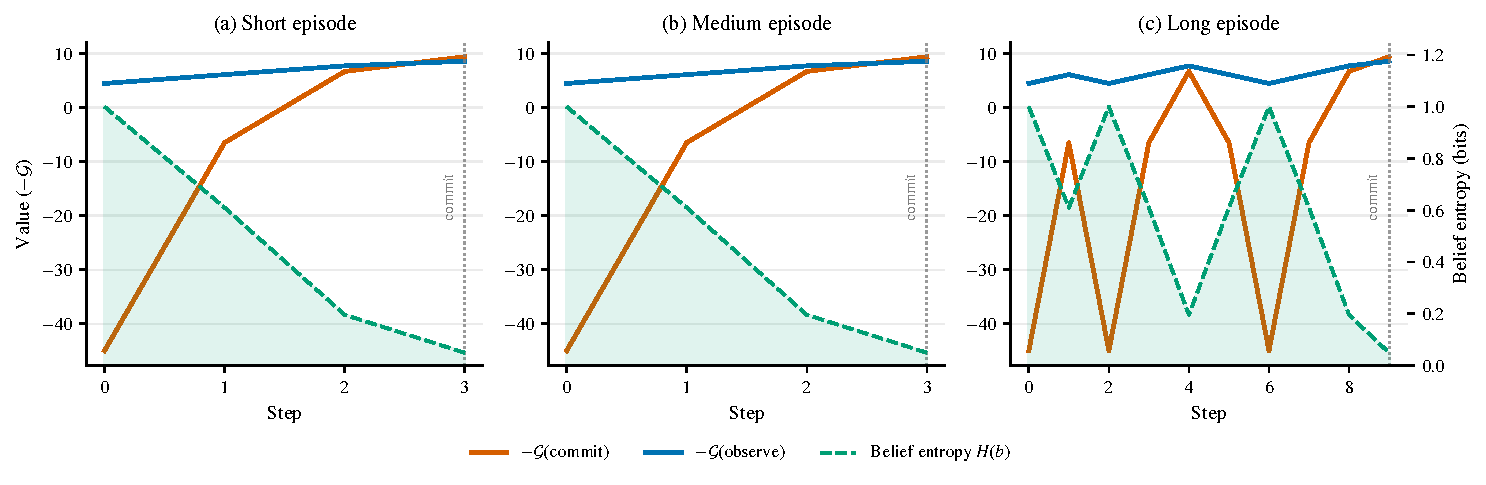
\includegraphics[width=0.78\linewidth]{figures/fig_efe_trajectory.pdf}
\caption{EFE decomposition within Tiger episodes ($H{=}6$). The agent commits at the crossover where commit value (red) exceeds observe value (blue). As belief entropy (green shading) decreases, the transition from exploration to exploitation occurs automatically.}
\label{fig:traj}
\Description{Three line plots for a short, a medium, and a long episode, each with a rising vermillion curve that starts near minus 45, a nearly flat blue curve near plus 5, and a green dashed entropy curve with light green fill plotted on a secondary axis. A dotted vertical line marks the step where the vermillion curve crosses above the blue one. In the short and medium panels the entropy declines steadily and the crossing occurs at step 3. In the long panel the vermillion curve and the entropy oscillate up and down several times before the crossing at step 9.}
\end{figure}

Figure~\ref{fig:traj} decomposes EFE within Tiger episodes. The agent commits at the crossover where commit value exceeds observe value. As belief entropy falls, the transition from exploration to exploitation happens on its own, with no stopping rule.

\subsection{Observation action scaling and adaptive test selection}
\label{app:obs_scaling}

\begin{figure}[htbp]
\centering
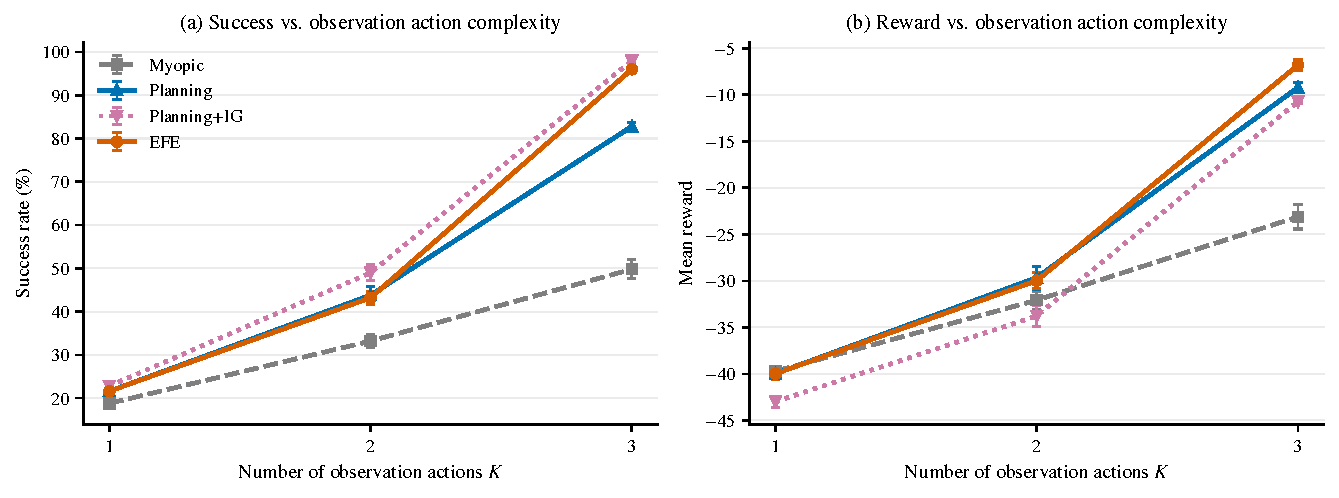
\includegraphics[width=0.78\linewidth]{figures/fig_obs_scaling.pdf}
\caption{Observation action scaling on Diagnosis ($N{=}8$, $H{=}3$, 500 episodes). EFE separates from Planning only once several tests compete. The gap is zero at $K{=}1$ (bit-identical policies), $-0.6$pp and within seed-level sampling error at $K{=}2$, and $+13.2$pp at $K{=}3$, where choosing among differentially informative tests is exactly what the information-gain term contributes.}
\label{fig:obs_scaling}
\Description{Two line plots against the number of observation actions, from 1 to 3. In the left panel success rates rise for all four agents, from roughly 19 to 23 percent at one action to about 96 to 98 percent for the vermillion and pink lines, 83 percent for the blue line, and about 50 percent for the gray line at three actions. In the right panel mean reward rises from between about minus 40 and minus 43 at one action to between about minus 7 and minus 23 at three actions, with the vermillion line ending highest and the pink dotted line starting lowest.}
\end{figure}

\begin{figure}[htbp]
\centering
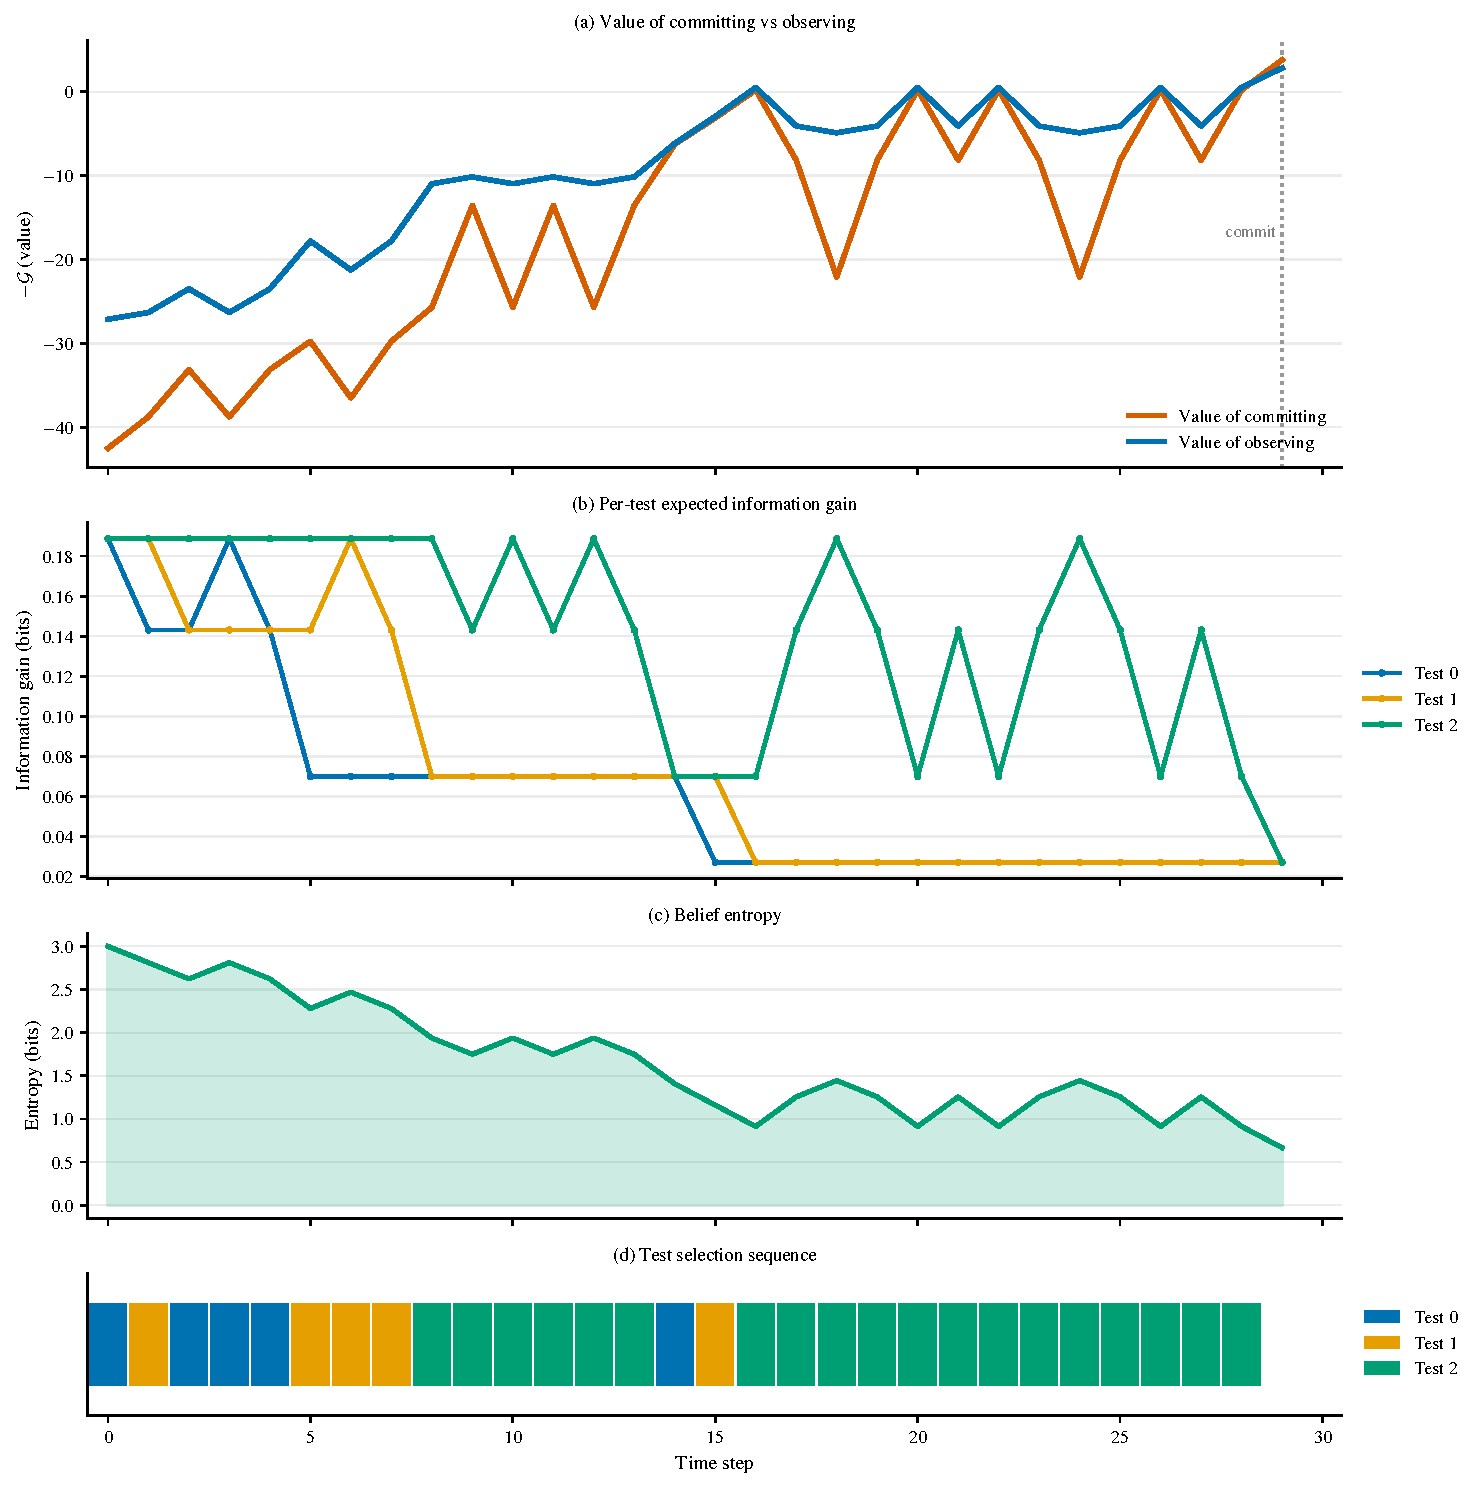
\includegraphics[width=0.78\linewidth]{figures/fig_extended_efe.pdf}
\caption{EFE decomposition over an extended Diagnosis episode ($N{=}8$, $K{=}3$). (a)~Value of committing vs.\ observing, where the agent commits at the crossover. (b)~Per-test expected information gain. Tests become differentially informative as belief concentrates, and the agent shifts its test selection as they do, though the recursive score it optimizes is not the one-step information gain plotted here. (c)~Belief entropy decay. (d)~Test selection sequence showing the agent's adaptive strategy.}
\label{fig:extended_efe}
\Description{Four stacked panels over roughly 30 time steps. In the top panel a vermillion curve rises from about minus 43 with repeated pronounced dips, touching a smoother blue curve several times before crossing it at a dotted vertical line at the final step. In the second panel three stepped lines for the three tests start near 0.19 bits, the blue and orange lines drop to about 0.03 bits at different times while the green line keeps oscillating between about 0.07 and 0.19 bits until the final step, so the green line stays at or above the other two for the whole episode. In the third panel a green entropy curve decays from 3 bits to under 1 bit with small bumps. The bottom strip is colored and encodes which test was chosen at each step, with runs of blue and orange early, then mostly green interrupted once near the middle by one blue and one orange step.}
\end{figure}

Holding $N{=}8$ fixed on Diagnosis and varying $K$ from 1 to 3 isolates the ``which information'' hypothesis (Figure~\ref{fig:obs_scaling}). At $K{=}1$ all agents face the same single test, and EFE and Planning are bit-identical. At $K{=}2$ the two remain within seed-level sampling error of each other ($43.2\%$ against $43.8\%$ success), with the multi-test evidence at that scale carried by the main Diagnosis battery (Section~\ref{sec:results}). The separation opens at $K{=}3$ ($96.0\%$ against $82.8\%$, $+13.2$pp), because selecting among competing tests is what the information-gain term contributes, a threshold rather than a steady growth. Figure~\ref{fig:extended_efe} shows the mechanism at work over a single extended episode. Tests become differentially informative as belief concentrates, since some partitions of the state space stop mattering once the condition is narrowed down while others remain decisive. The EFE agent tracks that structure and takes the most informative test still available at each step. This adaptive test selection is what underlies the advantage reported in Section~\ref{sec:results}.

\subsection{Reward asymmetry on Tiger}
\label{app:tiger_sweep}

\begin{figure}[htbp]
\centering
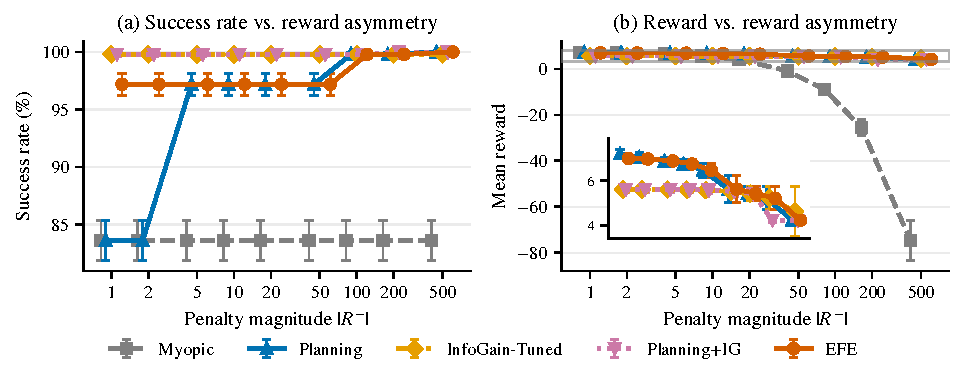
\includegraphics[width=0.78\linewidth]{figures/fig_asymmetry_sweep.pdf}
\caption{Reward asymmetry sweep on Tiger ($H{=}6$, 500 episodes per point, 5 canonical seeds). EFE and Planning adapt their listening as the penalty grows, with EFE rising from $2.7$ observations at $|R^-|{=}1$ to $5.8$ at $500$. The myopic InfoGain-Tuned agent at the fixed tuned weight listens $4.37$ times at every penalty, while Planning+IG at the same weight rises to $5.77$ at the two largest penalties. The myopic agent's fixed weight over-listens at low stakes, costing about $1.6$ reward against reward-only Planning at $|R^-|{=}1$, and its reward sits marginally ahead of EFE's only at the largest penalty, where it listens less ($4.37$ against $5.77$).}
\label{fig:sweep}
\Description{Two line plots against penalty magnitude on a log axis from 1 to 500, with five agents per panel. In the left panel the pink and orange lines hold near 100 percent success, the vermillion EFE line holds near 97 percent and joins them from a penalty of 100 onward, the blue Planning line steps up from about 84 percent to join EFE at a penalty of 5, and the gray dashed Myopic line stays flat near 84 percent. In the right panel every line runs flat near plus 5 to 7 except the gray Myopic line, which falls steadily to about minus 75 at the largest penalty.}
\end{figure}

To test whether EFE's Tiger parity holds across reward scales, we sweep the penalty magnitude from $|R^-|{=}1$ to $500$ (Figure~\ref{fig:sweep}). EFE adapts its listening on its own, from $2.7$ observations at the smallest penalty to $5.8$ at the largest, tracking the stakes without reconfiguration. The myopic InfoGain-Tuned agent, whose weight the sweep re-tunes at every penalty and which comes back as $w{=}20$ at all of them, listens $4.37$ times at every penalty, while the deeper Planning+IG at the same weight rises to $5.77$ observations at penalties $200$ and $500$. At low stakes that over-listening costs about $1.6$ reward against reward-only Planning. At the largest penalty the fixed-weight myopic agent sits marginally ahead of EFE ($4.61$ against $4.23$), so the case for adaptation is robustness across the sweep rather than uniform dominance.

\subsection{Belief evolution}
\label{app:tw_belief}

\begin{figure}[htbp]
\centering
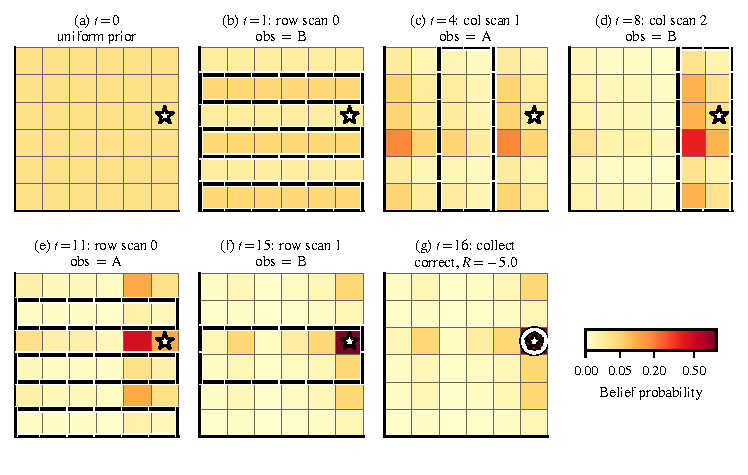
\includegraphics[width=0.78\linewidth]{figures/fig_tileworld_belief.pdf}
\caption{Belief evolution within an EFE episode on the $6{\times}6$ Tileworld. Each panel shows belief probability over the 36 grid cells (darker = higher probability) after successive scans. Blue outlines mark the scanned region. The agent concentrates belief toward the target tile (green star) and commits once confident.}
\label{fig:tw_belief}
\Description{A single row of seven six-by-six grids showing numeric belief values in every cell. The first grid is uniform at 0.03. Successive grids outline the scanned rows or columns in blue while values elsewhere shrink toward zero, with one cell reaching 0.47 in the fifth grid and the cell beside it reaching a dark red 0.73 in the sixth grid. The final grid shows the collect step with a green star on the committed cell.}
\end{figure}

\begin{figure}[htbp]
\centering
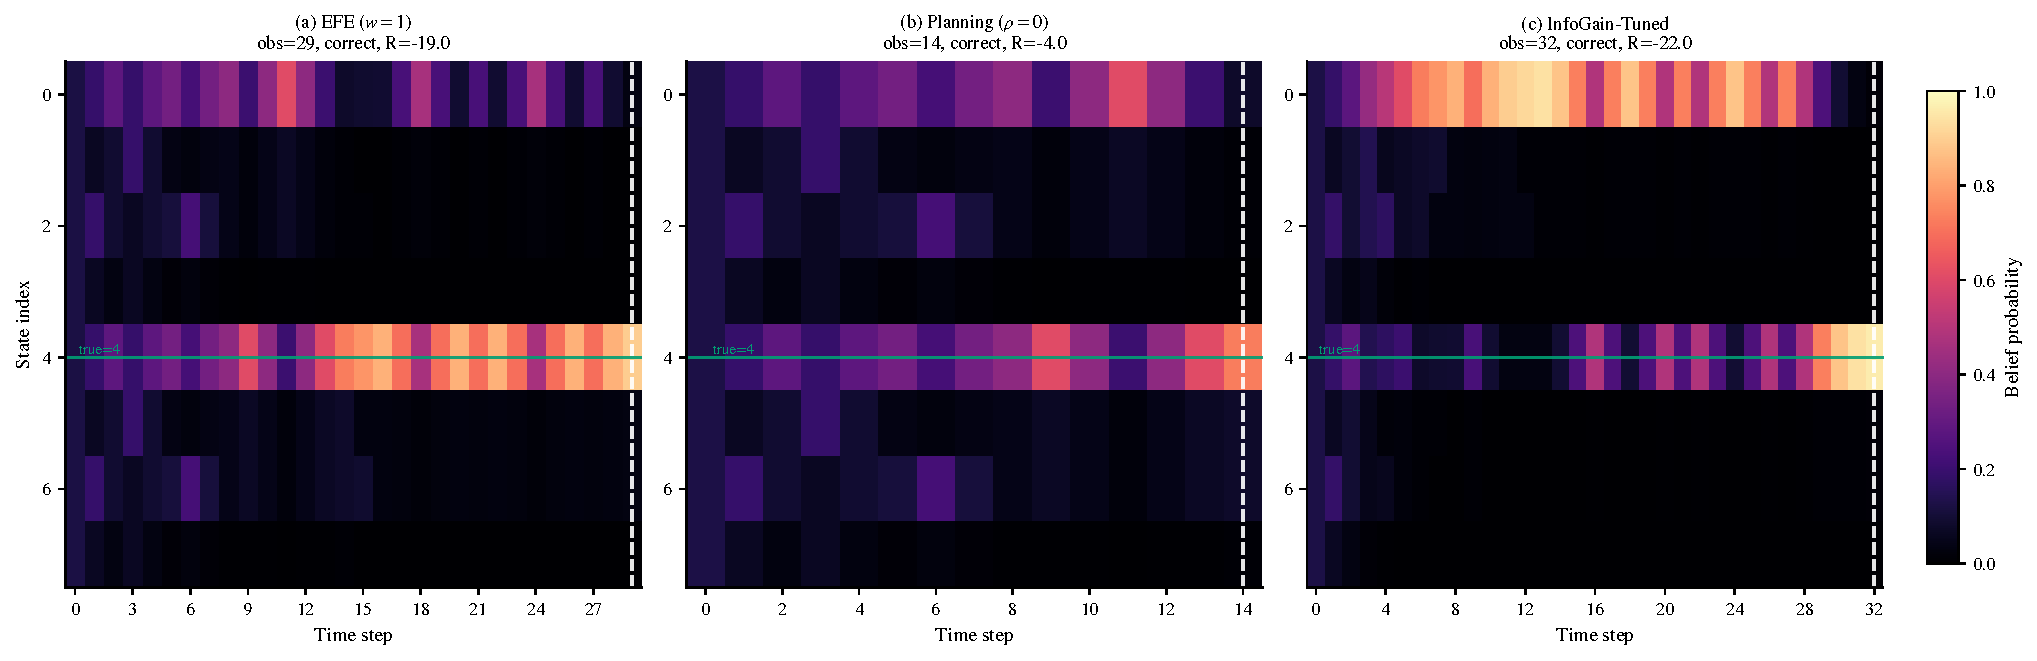
\includegraphics[width=0.78\linewidth]{figures/fig_belief_heatmap.pdf}
\caption{Belief evolution within representative Diagnosis episodes ($N{=}8$, $K{=}3$, accuracy 0.75). Brighter = higher probability. The green line marks the true state and the dashed line marks the commit point. EFE concentrates belief efficiently. InfoGain-Tuned over-explores.}
\label{fig:belief_heatmap}
\Description{Three heatmaps of state index, eight rows each, versus time step on a dark background, where brighter warm colors indicate higher belief. A horizontal green line marks the true state and a white dashed vertical line marks the commit step. In the left panel belief brightens steadily along the true state row and the EFE agent commits correctly at step 29. In the middle panel the Planning agent's belief brightens along the true state row and it commits correctly at step 14. In the right panel the brightest band sits on a wrong row for most of the episode, belief concentrates on the true state only near the end, and observations continue until step 32.}
\end{figure}

Figure~\ref{fig:tw_belief} follows belief within one EFE episode on the $6{\times}6$ Tileworld, and Figure~\ref{fig:belief_heatmap} does the same on extended Diagnosis instances ($N{=}8$, $K{=}3$, accuracy $0.75$) long enough for the plotted episode to run from fourteen to thirty-two observation steps across the three agents. EFE narrows by partition. Early tests eliminate large groups of states and later tests discriminate among what is left. Reward-only Planning commits before the belief has concentrated, and Info Gain keeps testing past the point where further tests change the decision.

\subsection{Exploration efficiency}
\label{app:foraging}

\begin{figure}[htbp]
\centering
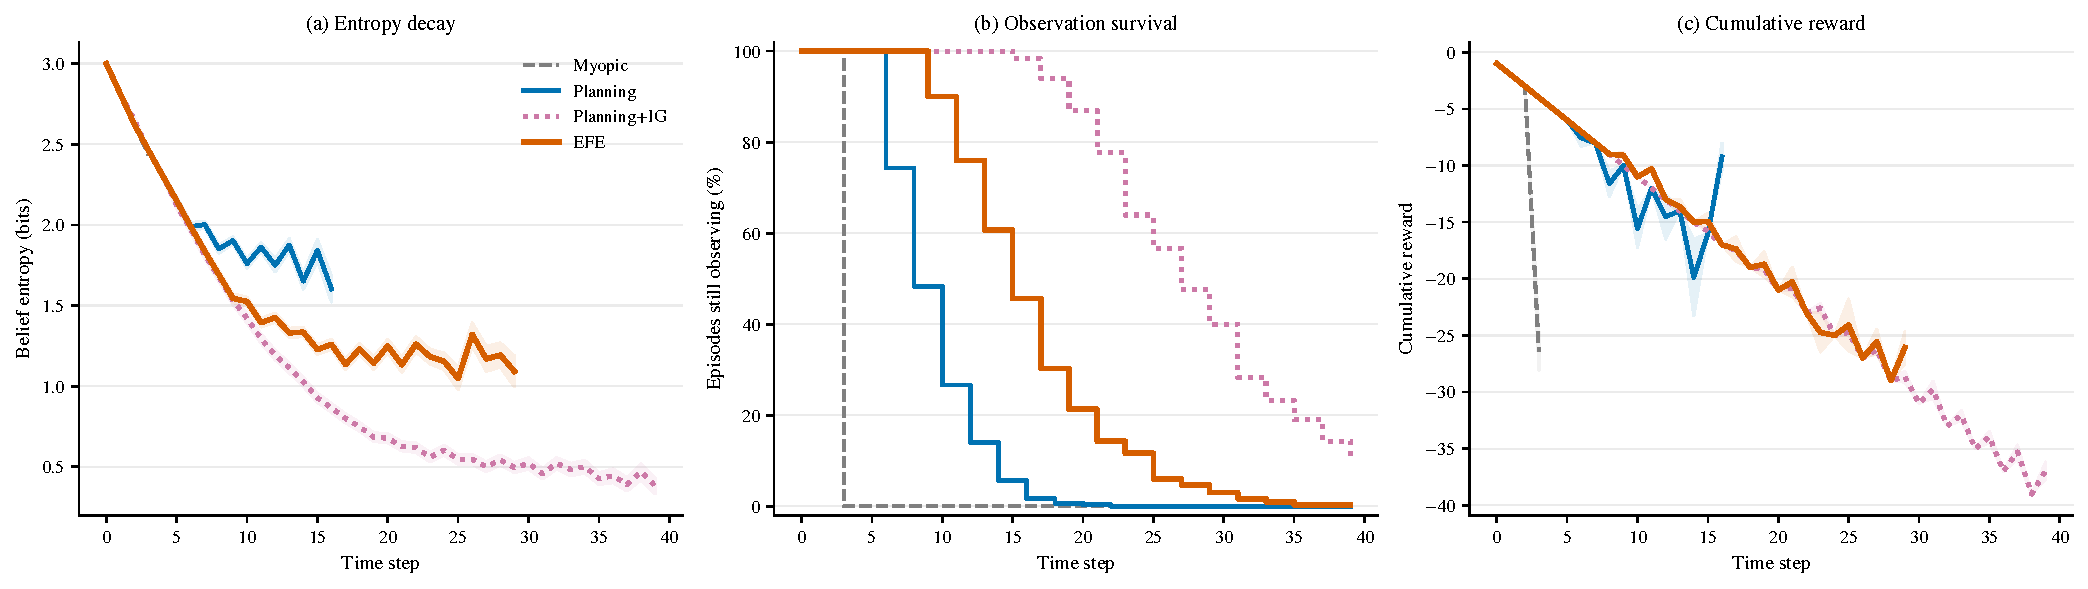
\includegraphics[width=0.78\linewidth]{figures/fig_efficiency_curves.pdf}
\caption{Exploration efficiency on Diagnosis ($N{=}8$, $K{=}3$, 300 episodes). (a) Belief entropy decay. (b) Fraction of episodes still observing. (c) Cumulative reward. EFE commits at the right time. Planning+IG over-explores.}
\label{fig:efficiency}
\Description{Three line plots over time steps. Left: belief entropy falls from 3 bits for all agents, with the blue line plateauing near 1.9 bits, the vermillion line declining to about 1 bit by step 30, and the pink dotted line falling lowest to about 0.5 bits. Middle: staircase survival curves of the fraction of episodes still observing, where the gray line drops to zero by step 3, the blue line by about step 15, the vermillion line by about step 35, and the pink line still shows over 10 percent observing at step 40. Right: cumulative reward declines roughly linearly for all agents, with the pink line extending furthest right and lowest, to about minus 40.}
\end{figure}

Figure~\ref{fig:efficiency} averages the temporal dynamics of epistemic foraging over 300 episodes. EFE reduces entropy at a rate comparable to tuned Planning+IG but commits earlier, staying out of the diminishing-returns regime. Its survival curve falls off through steps 10 to 25 while Planning+IG's extends further right.

\section{Environment specifications}
\label{app:envs}

\begin{table}[htbp]
\centering
\caption{Full environment specifications for every environment reported in the main results tables. Variant instances used outside the main results tables (Navigation $5{\times}5$ and $7{\times}7$, Tileworld $4{\times}4$, Diagnosis $N \in \{2,8,16\}$) differ from their tabulated siblings only in the stated size parameter. $H$ is the planning horizon for observe-then-commit environments and the tree depth for the interleaved ones. $\gamma$ is the discount used by the reporting agents. All main-text batteries are undiscounted ($\gamma{=}1.0$, the agent default), and $\gamma$ is set to $0.999$ inside the SARSOP/CPOMDP exports of Section~\ref{sec:sarsop}, which require a discounted infinite-horizon model, and is otherwise varied only in the discount sweep of Appendix~\ref{app:discount} and in two rows of the RockSample POMCP sensitivity battery. $|S|$ counts hidden-state configurations only, excluding fully observable components such as the RockSample agent position.}
\resizebox{\linewidth}{!}{%
\begin{tabular}{lcccccccc}
\toprule
Environment & $|S|$ & Obs.\ actions & Commit actions & Accuracy & Obs.\ cost & Correct & Incorrect & $H$ / $\gamma$ \\
\midrule
Tiger & 2 & 1 & 2 & 0.85 & $-1.0$ & $+10$ & $-100$ & 6 / 1.0 \\
Testbed & 2 & 1 & 2 & 0.75 & $-0.1$ & $+1$ & $-1$ & 4 / 1.0 \\
Diagnosis ($N{=}4$) & 4 & 2 & 4 & 0.80 & $-1.0$ & $+10$ & $-50$ & 3 / 1.0 \\
Bandit ($K{=}4$) & 4 & 4 & 4 & 0.80 & $-0.5$ & $+10$ & $+1$ & 2 / 1.0 \\
Navigation & 9 & 4 (move) & 0 (implicit) & var. & $-0.5$ & $+20$ & -- & 2 / 1.0 \\
Tileworld ($6{\times}6$) & 36 & 6 (scan) & 36 (collect) & 0.80 & $-1.0$ & $+10$ & $-50$ & 2 / 1.0 \\
Tileworld ($8{\times}8$) & 64 & 6 (scan) & 64 (collect) & 0.80 & $-1.0$ & $+10$ & $-50$ & 2 / 1.0 \\
\midrule
\multicolumn{9}{l}{\emph{Interleaved observe-act (Proposition~\ref{prop:factored}). Undiscounted. Every RockSample action costs $-0.5$, and Inspection's per-action costs are given in its own rows}} \\
RockSample RS[5,3] & $2^{3}{=}8$ & 3 (check) & sample/exit & $0.95$ decaying & $-0.5$ & $+10$ & $-10$ & 3 / 1.0 \\
RockSample RS[7,4] & $2^{4}{=}16$ & 4 (check) & sample/exit & $0.95$ decaying & $-0.5$ & $+10$ & $-10$ & 4 / 1.0 \\
RockSample RS[7,8] & $2^{8}{=}256$ & 8 (check) & sample/exit & $0.95$ decaying & $-0.5$ & $+10$ & $-10$ & 3 / 1.0 \\
RockSample RS[11,11] & $2^{11}{=}2{,}048$ & 11 (check) & sample/exit & $0.95$ decaying & $-0.5$ & $+10$ & $-10$ & 2 / 1.0 \\
Inspection ($N{=}8$) & $2^{8}{=}256$ & 2 types $\times$ 8 & diagnose & $0.70 / 0.90$ & $-0.5 / -2.0$ & $+5$ fault & $-50$ missed & 3 / 1.0 \\
Inspection ($N{=}16$) & $2^{16}{=}65{,}536$ & 2 types $\times$ 16 & diagnose & $0.70 / 0.90$ & $-0.5 / -2.0$ & $+5$ fault & $-50$ missed & 2 / 1.0 \\
\bottomrule
\end{tabular}}
\end{table}

RockSample check accuracy decays with distance from the rock ($0.95$ at range zero, halving every $4$ cells, floored at $0.5$). The tabulated value is the maximum. Each RockSample instance runs under an episode step cap of $N^2 + 10K$ steps, giving $55$, $89$, $129$, and $231$ for RS[5,3], RS[7,4], RS[7,8], and RS[11,11], and the fixed rock maps are those in \texttt{ROCKSAMPLE\_CONFIGS} (\texttt{experiments/run\_rocksample.py}). On RS[11,11] the start cell $(5,0)$ coincides with a rock while every other rock lies at Euclidean distance $3.16$ or more, at or beyond the limit of the sensor's useful range (accuracy roughly $0.55$ at distance $3.16$, and floored at chance from $3.7$ cells), the geometry behind the single-informative-check pattern of Section~\ref{sec:rocksample}. Its per-instance tree depth was fixed a priori before the reported runs, not selected on measured agent performance, and the depth-3 check on RS[11,11] (Section~\ref{sec:rocksample}) shows the reported pattern is insensitive to one extra ply. Inspection additionally pays $-0.5$ per move, gives $+2$ for a correct nominal call, and $-5$ for a false alarm, with fault prior $0.3$.

All environments are implemented as Gymnasium \citep{towers2024} environments with the standard \texttt{reset}/\texttt{step} API. The Diagnosis environment uses $K = \lceil \log_2 N \rceil$ binary tests, each providing noisy information about a different partition of the state space. The Navigation environment uses proximity-based warm/cold signals with accuracy depending on Manhattan distance to the hidden goal. The Tileworld projects the Diagnosis partition structure onto a 2D grid. $K = 2 \lceil \log_2 n \rceil$ scans, for grid side $n$, partition the grid by bit-level splits of the row and column indices, enabling complete spatial disambiguation.

\section{Navigation results}
\label{app:navigation}

Navigation uses only move actions. The goal cell is hidden, and each move yields a proximity-based warm/cold observation (Section~\ref{app:envs}). Unlike Diagnosis or Tileworld, there is no separate menu of observation actions. Information arrives as a side effect of translation, and greedy progress toward the belief mode already provides correlated evidence.

\begin{table}[htbp]
\centering
\caption{Navigation scaling ($150$ episodes per seed $\times$ $5$ seeds = $750$ episodes per agent per grid). Step budget $3n^2$. NavEFE uses depth-limited planning $H{=}2$. Uncertainty is seed-level SE. See \texttt{results\_navigation\_scaling.csv} and the companion seed-level Welch tests in \texttt{results\_navigation\_scaling\_seed\_stats.csv}.}
\label{tab:nav_scaling}
%% Numbers in this table are produced by experiments/run_experiment.py navigation-scaling
\begin{small}
\begin{tabular}{lcccc}
\toprule
Grid & $|S|$ & Agent & Success & Mean reward \\
\midrule
\multirow{3}{*}{$3{\times}3$} & \multirow{3}{*}{$9$} & NavMyopic & $90.4 \pm 1.3\%$ & $+2.04 \pm 1.51$ \\
& & NavInfoGain & $86.4 \pm 1.6\%$ & $-1.37 \pm 1.69$ \\
& & NavEFE ($H{=}2$) & $87.2 \pm 1.7\%$ & $-1.29 \pm 1.58$ \\
\midrule
\multirow{3}{*}{$5{\times}5$} & \multirow{3}{*}{$25$} & NavMyopic & $80.7 \pm 1.4\%$ & $-16.64 \pm 1.54$ \\
& & NavInfoGain & $76.0 \pm 1.5\%$ & $-23.24 \pm 1.75$ \\
& & NavEFE ($H{=}2$) & $74.4 \pm 1.2\%$ & $-25.76 \pm 1.14$ \\
\midrule
\multirow{3}{*}{$7{\times}7$} & \multirow{3}{*}{$49$} & NavMyopic & $65.7 \pm 2.8\%$ & $-38.42 \pm 2.77$ \\
& & NavInfoGain & $60.3 \pm 1.2\%$ & $-44.28 \pm 1.12$ \\
& & NavEFE ($H{=}2$) & $62.8 \pm 0.7\%$ & $-40.86 \pm 0.77$ \\
\bottomrule
\end{tabular}
\end{small}
\end{table}

NavMyopic (move toward the highest-probability cell) is the strongest baseline at every scale, nominally at $3{\times}3$ and $7{\times}7$ and significantly at $5{\times}5$, where its lead over NavEFE holds on reward ($p{=}0.002$), success ($p{=}0.010$), and observation count ($p{=}0.001$, all seed-level Welch, Holm-corrected within metric at each grid size, \texttt{results\_navigation\_scaling\_seed\_stats.csv}). At the other two sizes no pairwise difference survives correction at 5 seeds. Extra steps devoted to exploratory detours incur the per-move cost without the sharp information returns seen when tests can be chosen explicitly, and at no size does an epistemic agent significantly beat the myopic rule. This is not a failure of $w{=}1$ so much as a structural regime change relative to our main benchmarks. NavEFE is competitive with one-step NavInfoGain at $7{\times}7$, with nominally higher mean reward ($-40.86$ against $-44.28$, seed-level $p{=}0.040$ uncorrected, not significant after Holm) and comparable success, evidence that recursive epistemic valuation is not harmful once the grid is large enough that myopic information gain is already costly. The contrast with Tileworld (Figure~\ref{fig:tw_scaling}) underscores the multiple-observation-actions condition of Section~\ref{sec:discussion}. EFE's clearest wins appear when the agent must select among differentially informative observation actions, not only where to translate next under a smooth proximity field.

\section{Scaling analysis}
\label{app:scaling}

\begin{table}[htbp]
\centering
\caption{Scaling analysis. Diagnosis $N = 2$ to $16$ (2{,}500 episodes at 500 per seed $\times$ 5 seeds, $H{=}2$). Bold marks the best success and reward per $N$ and the tests of those rows, plus any row within sampling error of it (seed-level Welch $p > 0.05$, uncorrected, \texttt{results\_scaling\_stats.csv}). At $N{=}8$ and $N{=}16$ the EFE and Planning rows are statistical ties.}
\begin{small}
\begin{tabular}{clccc}
\toprule
$N$ & Agent & Tests & Success & Reward \\
\midrule
\multirow{4}{*}{2}  & Myopic    & 1.00 & 80.3\% & $-2.83$ \\
                     & \textbf{Planning}  & \textbf{2.91} & \textbf{94.1\%} & $\mathbf{+3.56}$ \\
                     & Info Gain & 1.00 & 80.3\% & $-2.83$ \\
                     & \textbf{EFE} & \textbf{2.91} & \textbf{94.1\%} & $\mathbf{+3.56}$ \\
\midrule
\multirow{4}{*}{4}  & Myopic & 2.00 & 64.5\% & $-13.29$ \\
                     & \textbf{Planning} & \textbf{5.83} & \textbf{88.8\%} & $\mathbf{-2.58}$ \\
                     & Info Gain & 2.00 & 64.5\% & $-13.29$ \\
                     & \textbf{EFE} & \textbf{5.83} & \textbf{88.8\%} & $\mathbf{-2.58}$ \\
\midrule
\multirow{4}{*}{8}  & Myopic & 3.00 & 51.1\% & $-22.33$ \\
                     & \textbf{Planning} & \textbf{8.79} & \textbf{83.9\%} & $\mathbf{-8.44}$ \\
                     & Info Gain & 3.00 & 51.1\% & $-22.33$ \\
                     & \textbf{EFE} & \textbf{8.83} & \textbf{84.1\%} & $\mathbf{-8.38}$ \\
\midrule
\multirow{4}{*}{16} & Myopic & 4.00 & 40.8\% & $-29.50$ \\
                     & \textbf{Planning} & \textbf{11.65} & \textbf{77.4\%} & $\mathbf{-15.23}$ \\
                     & Info Gain & 4.00 & 40.8\% & $-29.50$ \\
                     & \textbf{EFE} & \textbf{11.64} & \textbf{77.1\%} & $\mathbf{-15.37}$ \\
\bottomrule
\end{tabular}
\end{small}
\end{table}

At $H{=}2$, EFE and Planning show no consistent gap at any $N$ tested here (bit-identical at $N{=}2$ and $N{=}4$, at $N{=}8$, $84.08\% \pm 0.66$pp vs.\ $83.92\% \pm 0.82$pp, and at $N{=}16$, $77.12\% \pm 0.78$pp vs.\ $77.36\% \pm 0.98$pp, seed-level SE, with no consistent direction), both substantially outperforming Myopic and untuned Info Gain. This contrasts with the $H{=}3$ Diagnosis result (Table~\ref{tab:main}), where EFE outperformed Planning by $+8.3$ pp, confirming that EFE's advantage requires sufficient recursive depth, not merely a larger state space. EFE-over-Myopic advantage grows from $+13.8$ pp at $N{=}2$ ($94.12\% \pm 0.50$pp vs.\ $80.28\% \pm 0.91$pp) to $+36.3$ pp at $N{=}16$ ($77.12\% \pm 0.78$pp vs.\ $40.84\% \pm 1.69$pp, seed-level SE), confirming that deeper planning is increasingly valuable as state spaces grow, independent of whether EFE or reward-only Planning supplies that depth.

\section{PyMDP consistency check}
\label{app:pymdp}

We check our EFE computation against the \texttt{pymdp} library \citep{heins2022} by wrapping pymdp's standard Agent class. This is a consistency check, not a certified numerical equivalence, and we state its strength precisely rather than leaving ``validated'' to do unearned work. The quantitative form of the check is a deployed comparison on the two-state testbed. Run as an ordinary observe-then-commit agent over the canonical protocol, \texttt{pymdp}-AIF returns $3.15$ observations, $89.8\%$ success, and $+0.480$ reward, bit-identical to reward-only Planning on all three metrics (\texttt{results\_summary.csv}). The meaningful comparator here is our own myopic Info Gain agent at $w{=}1$, which \texttt{results\_summary.csv} records at the same $3.15$ observations, $89.8\%$ success, and $+0.480$ reward. Both agents evaluate single-step policies, and by Proposition~\ref{prop:equivalence} the myopic $w{=}1$ agent is the myopic EFE agent, so this is a like-for-like agreement. Our $H{=}4$ recursive EFE agent legitimately differs on this environment ($5.50$ observations), through planning depth rather than through any disagreement about the epistemic term. The check is therefore evidence that the two myopic implementations agree, not that recursive EFE matches pymdp. It remains weak evidence, since on this environment the myopic $w{=}1$ agent is itself bit-identical to reward-only Planning, so the comparison cannot separate a correctly implemented epistemic term from its absence. Both implementations agree on observe-vs-commit decisions across all tested belief states (uniform, intermediate, and confident beliefs on the two-state environments). Information gain values computed by our recursive scheme and pymdp's \texttt{control} module agree qualitatively, with differences attributable to our recursive multi-step evaluation vs.\ pymdp's single-step policy enumeration.

\section{Supplementary statistics}
\label{app:stats}

Pairwise comparisons in the main results tables use independent two-sample Welch $t$-tests on per-seed means with Holm--Bonferroni correction for family-wise error control, and comparisons reported without that correction are marked uncorrected where they appear. The companion pooled episode-level column in the six stats files behind the main observe-then-commit and Tileworld tables is an equal-variance two-sample test rather than a Welch test, which changes no non-degenerate comparison's outcome at $\alpha{=}0.05$ across the $510$ pooled comparisons in those files. The RockSample and Structural Inspection producers use Welch for both levels. The correction family is the full set of pairwise agent comparisons and metrics (reward, success/accuracy, and, where reported, observation count) reported together within a single table. For the main results tables (Table~\ref{tab:main} and the RockSample and Structural Inspection tables), the family is scoped to one environment or instance at a time, since each table's rows are computed and corrected together, independently of every other table. Concretely, with $A$ agents and $M$ corrected metrics the family size is $M \cdot \binom{A}{2}$. $108$ for Tiger ($A{=}9$, $M{=}3$ over reward, success, and observations), $84$ for Diagnosis and Bandit ($A{=}8$, $M{=}3$), and $18$ for each Structural Inspection instance ($A{=}4$, $M{=}3$ over reward, accuracy, and tests). RockSample corrects within metric rather than pooling, giving $28$ tests per metric per instance over its eight agents, because the RockSample table's bolding rule treats a non-rejection as a tie with the best row and pooling metrics into one larger family would loosen exactly that rule. The exception is the discount-sweep appendix table (Table~\ref{tab:discount}), where the family spans every environment and $\gamma$ value in that sweep jointly ($24$ tests, from $3$ environments $\times$ $4$ discount factors $\times$ $2$ metrics), since those rows are accumulated and corrected together before the table is written. Bootstrap 95\% confidence intervals use 10{,}000 resamples with fixed seed for reproducibility. Effect sizes use Cohen's $d$ with pooled standard deviation. Because episodes within a seed are not independent, those primary tests aggregate each seed's episodes to a single mean before testing ($n{=}5$ seeds), and the pooled episode-level columns are reported alongside them. The main-text table (Table~\ref{tab:main}) reports the seed-level SE as the primary uncertainty measure, since each answers a different question (episode-level precision versus between-seed replicability) and neither alone is a strict superset of the other. The Tiger, Diagnosis and Bandit tables of Appendix~\ref{app:full_tables} report the pooled episode-level SE only and omit the untuned Info Gain rows that duplicate Myopic exactly, together with Tiger's pymdp-AIF row. The two Tileworld tables report point estimates for every agent run, duplicates included. The companion \texttt{*\_stats.csv} files committed alongside the main battery carry the seed-level Welch $t$-tests and Cohen's $d$ this section describes. The Tileworld scaling battery reports seed-level standard errors for reward and success without a companion Welch file.

\begin{table}[htbp]
\centering
\caption{Cohen's $d$ for EFE vs.\ each baseline on mean episode reward (top) and vs.\ Planning on success rate (bottom). Positive $d$ favors EFE. Interpretation. $|d|{<}0.2$ negligible, $0.2$--$0.5$ small, $0.5$--$0.8$ medium, $|d|{>}0.8$ large. Success-rate $d$ uses the same pooled-$s$ convention as reward (proportions treated as per-episode Bernoulli outcomes).}
\label{tab:effect_sizes}
%% Numbers in this table are produced by experiments/run_supplementary.py
\begin{small}
\begin{tabular}{llrl}
\toprule
Environment & Comparison & $d$ (reward) & Interpretation \\
\midrule
Tiger & EFE vs.\ Myopic & $+0.44$ & small \\
Tiger & EFE vs.\ Planning & $0.00$ & negligible (exact tie) \\
Tiger & EFE vs.\ InfoGain-Tuned & $0.00$ & negligible (exact tie) \\
Tiger & EFE vs.\ Planning+IG & $+0.14$ & negligible \\
Tiger & EFE vs.\ Posterior-vote & $+0.09$ & negligible \\
\midrule
Testbed & EFE vs.\ Myopic & $-0.07$ & negligible \\
Testbed & EFE vs.\ Planning & $-0.18$ & negligible \\
Testbed & EFE vs.\ InfoGain-Tuned & $+0.69$ & medium \\
Testbed & EFE vs.\ Planning+IG & $+0.69$ & medium \\
Testbed & EFE vs.\ Posterior-vote & $-0.18$ & negligible \\
\midrule
Diagnosis & EFE vs.\ Myopic & $+0.55$ & medium \\
Diagnosis & EFE vs.\ Planning & $+0.08$ & negligible \\
Diagnosis & EFE vs.\ InfoGain-Tuned & $+0.25$ & small \\
Diagnosis & EFE vs.\ Planning+IG & $+0.25$ & small \\
Diagnosis & EFE vs.\ Posterior-vote & $+0.09$ & negligible \\
\midrule
Bandit & EFE vs.\ Myopic & $+0.18$ & negligible \\
Bandit & EFE vs.\ Planning & $+0.14$ & negligible \\
Bandit & EFE vs.\ InfoGain-Tuned & $+0.36$ & small \\
Bandit & EFE vs.\ Planning+IG & $+0.37$ & small \\
Bandit & EFE vs.\ Posterior-vote & $-0.01$ & negligible \\
\midrule
\multicolumn{4}{l}{\textit{Success rate} ($d$ favors EFE)} \\
\midrule
Tiger & EFE vs.\ Planning & $0.00$ & negligible (exact tie) \\
Testbed & EFE vs.\ Planning & $+0.26$ & small \\
Diagnosis & EFE vs.\ Planning & $+0.33$ & small \\
Bandit & EFE vs.\ Planning & $+0.40$ & small \\
\bottomrule
\end{tabular}
\end{small}
\end{table}

The reward table shows that EFE vs.\ Planning is negligible to none on Tiger, Diagnosis, and Bandit (exactly zero on Tiger, where EFE and Planning tie). Once both agents take enough informative actions, mean returns are similar, even though success rates differ. The success-rate rows isolate the axis where EFE improves most relative to Planning on Diagnosis and Bandit. Against over-exploring tuned alternatives (InfoGain-Tuned, Planning+IG), EFE shows medium reward effects on the Testbed ($d = 0.69$) and small effects on Bandit ($d \approx 0.36$-$0.37$), reflecting the cost of over-exploration at Bandit's success-tuned weight of $w{=}20$.

\section{Near-optimality across planning horizons}
\label{app:nearopt_horizon}

Proposition~\ref{prop:nearopt} bounds $w^*_{\mathrm{lo}}$ at $H{=}1$ and $w^*_{\mathrm{hi}}$ at $H{=}2$. To check whether the resulting near-optimality claim survives recursive multi-step planning, we generated 100 random two-state environments (reward asymmetry $\alpha \in [1,50]$, observation accuracy $p \in [0.55, 0.95]$, cost $\in [0.1, 5]$) and, for each environment and each $H \in \{1,2,3\}$, computed the reward-optimal weight $w^*$ by grid search and recorded whether $w{=}1$ falls within $\max(5\%, 0.5)$ of the best achievable reward. Each (environment, weight, horizon) cell runs $50$ episodes at a single seed, and $w^*$ is selected over the six-point grid $\{0.01, 0.5, 1, 2, 5, 50\}$ (\url{experiments/run_nearopt_horizon.py}). This is a deliberate deviation from the canonical five-seed protocol, because the study is a descriptive sweep over $100$ synthetic environments rather than a headline comparison, and its conclusions are read as coarse rates rather than per-environment estimates. Figure~\ref{fig:nearopt_horizon} reports the fraction of environments where $w{=}1$ passes this test at each horizon, stratified by $\alpha$. The near-optimality rate rises from 30\% at $H{=}1$ to 58\% at $H{=}2$ and 79\% at $H{=}3$ (26\%~$\to$~53\%~$\to$~79\% restricted to $\alpha \geq 10$), so deeper planning widens the basin in which the untuned information-unit weight is reward-competitive rather than narrowing it. This is the same trend reported for Bandit in Section~\ref{sec:discussion}, where the low reward asymmetry predicts only marginal $H{=}1$ sufficiency yet multi-step EFE performs well in practice.

\begin{figure}[ht]
\centering
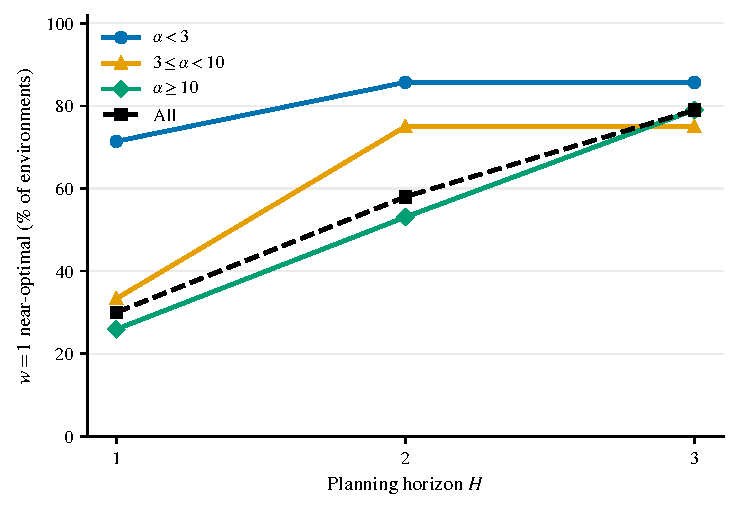
\includegraphics[width=0.7\linewidth]{figures/fig_nearopt_horizon.pdf}
\caption{Fraction of randomly generated two-state environments where $w{=}1$ is near-optimal, as a function of planning horizon $H$, stratified by reward asymmetry $\alpha$. The near-optimality basin widens with horizon, confirming that multi-step planning amplifies the value of observation. 100 environments, $\alpha \in [1,50]$, $p \in [0.55, 0.95]$, cost $\in [0.1, 5]$.}
\label{fig:nearopt_horizon}
\Description{A line plot of the percentage of environments passing the near-optimality test against planning horizon values 1, 2, and 3. A dashed black line for all environments rises from about 30 to 79 percent. Of the three colored strata, the blue line (low reward asymmetry) rises from about 71 to 86 percent and flattens, the orange line (moderate asymmetry) rises from about 33 to 75 percent and flattens, and the green line (high asymmetry) rises steadily from about 26 to 79 percent without flattening.}
\end{figure}

\paragraph{Horizon map: where myopic and deeper planning agree, and where they do not.} Figure~\ref{fig:nearopt_horizon} stratifies only by reward asymmetry $\alpha$. Table~\ref{tab:horizon-map} breaks the same 100 environments down by all three sampled regime axes and adds a direct per-environment comparison of the $H{=}1$ classification against $H{\geq}2$. Eight of the nine regime strata show the same qualitative pattern, with near-optimality rarer at $H{=}1$ than at $H{=}3$. The effect is sharpest for high-informativeness observations ($p \geq 0.85$, rising $17\% \to 90\%$). The exception is the low-informativeness stratum ($p < 0.65$, $25$ environments), which is flat and mildly non-monotone at $80\% \to 84\% \to 80\%$, since weak observations leave little for a deeper horizon to exploit. Low reward asymmetry rises but less sharply ($\alpha < 3$, from $71\%$ at $H{=}1$ to $86\%$ by $H{=}2$, holding there through $H{=}3$, on 7 environments). The per-environment comparison uses the producing script's definition of agreement. An environment agrees when $w{=}1$ is near-optimal at $H{=}1$ and at some deeper horizon, or at neither. By that definition the two horizons agree on 44 of the 100 environments. In 30 the $H{=}1$ check passes and near-optimality recurs at some deeper horizon, and in 26 of those 30 it holds at every deeper horizon tested. In 14 the check fails and never recovers. The remaining 56 environments fail the $H{=}1$ check yet turn out near-optimal at some deeper horizon (myopic underclaiming, the safe direction, a missed opportunity rather than a risk). On this random sample, zero environments show the opposite pattern (myopic overclaiming, where $H{=}1$ predicts near-optimality but no deeper horizon delivers it). Four of the 30 passers fail at exactly one of the two deeper horizons (environments 2, 42, 63, and 95 in the committed CSV), so a practitioner validating $w{=}1$ with a cheap $H{=}1$ check would have been misled at one specific deeper horizon in 4 of 30 cases, and in no case toward a weight that fails at every deeper horizon. This is a property of the observed sample, not a proven guarantee. We report it as an empirical boundary map over one random family of two-state environments, not an adaptive-submodularity result, and we make no claim that the $H{=}1$ check is monotone or that overclaiming is impossible in general, only that it did not occur here (the per-environment data is in \texttt{results/results\_nearopt\_horizon.csv}, from which \texttt{experiments/build\_horizon\_map.py} derives the aggregate agreement counts in \texttt{results/results\_horizon\_map\_agreement.csv}).

% Table auto-generated by experiments/build_horizon_map.py from
% results/results_nearopt_horizon.csv -- see that script to regenerate.
% Auto-generated by experiments/build_horizon_map.py -- do not edit by hand.
\begin{table}[t]
\centering
\caption{Horizon map: fraction of randomly generated two-state environments
 where $w{=}1$ is near-optimal (within $\max(5\%, 0.5)$ of the
 reward-optimal weight), stratified by each sampled regime axis and
 planning horizon $H$. Same 100 environments as Figure~\ref{fig:nearopt_horizon}
 (Appendix~\ref{app:nearopt_horizon}); this is an empirical boundary map, not an
 adaptive-submodularity guarantee.}
\label{tab:horizon-map}
\small
\begin{tabular}{lccc}
\toprule
Regime & $H{=}1$ & $H{=}2$ & $H{=}3$ \\
\midrule
\multicolumn{4}{l}{\textit{$\alpha$ (reward asymmetry)}} \\
\quad $\alpha<3$ & 0\% & 43\% & 29\% \\
\quad $3 \le \alpha < 10$ & 0\% & 25\% & 50\% \\
\quad $\alpha \ge 10$ & 14\% & 19\% & 37\% \\
\multicolumn{4}{l}{\textit{$p$ (observation informativeness)}} \\
\quad $p<0.65$ & 20\% & 8\% & 24\% \\
\quad $0.65 \le p < 0.85$ & 11\% & 9\% & 31\% \\
\quad $p \ge 0.85$ & 3\% & 50\% & 60\% \\
\multicolumn{4}{l}{\textit{cost (observation cost)}} \\
\quad cost$<1$ & 5\% & 16\% & 42\% \\
\quad $1 \le$ cost$<3$ & 5\% & 18\% & 37\% \\
\quad cost$\ge 3$ & 19\% & 26\% & 37\% \\
\bottomrule
\end{tabular}
\par\vspace{2pt}\footnotesize $H{=}1$ vs.\ $H{\geq}2$ agreement: 50\% of 100 environments agree; myopic overclaims 8, underclaims 42.
\end{table}


\section{Discount factor sensitivity}
\label{app:discount}

We test EFE and Planning agents' sensitivity to discounting by sweeping $\gamma \in \{0.9, 0.95, 0.99, 1.0\}$ across three environments, at the canonical 5-seed protocol. Including Planning at each $\gamma$ enables comparison of the relative gap between agents under discounting.

\begin{table}[htbp]
\centering
\caption{EFE and Planning agent performance across discount factors $\gamma$ (2{,}500 episodes at 500 per seed $\times$ 5 seeds, lighter than Table~\ref{tab:main}'s 5{,}000-episode battery, so small numeric differences from that table on the $\gamma{=}1.0$ row are expected). $\Delta$Succ.\ shows the success rate gap (EFE $-$ Planning) at each $\gamma$, with the seed-level Welch $p$-value in parentheses. $^*$ marks significance after Holm--Bonferroni correction.}
\label{tab:discount}
%% Numbers in this table are produced by experiments/run_discount.py
\begin{small}
\begin{tabular}{llccccc}
\toprule
Environment & Agent & $\gamma$ & Obs. & Success & Reward & $\Delta$Succ. ($p$) \\
\midrule
\multirow{8}{*}{Tiger}
& EFE & 0.90 & 4.23 & 99.6\% & $+5.33$ & \multirow{2}{*}{$+2.7$ ($p<10^{-3}$)$^*$} \\
& Planning & 0.90 & 2.65 & 96.9\% & $+3.91$ & \\
& EFE & 0.95 & 4.23 & 99.6\% & $+5.33$ & \multirow{2}{*}{$0.0$ ($p{=}1.0$)} \\
& Planning & 0.95 & 4.23 & 99.6\% & $+5.33$ & \\
& EFE & 0.99 & 4.23 & 99.6\% & $+5.33$ & \multirow{2}{*}{$0.0$ ($p{=}1.0$)} \\
& Planning & 0.99 & 4.23 & 99.6\% & $+5.33$ & \\
& EFE & 1.00 & 4.23 & 99.6\% & $+5.33$ & \multirow{2}{*}{$0.0$ ($p{=}1.0$)} \\
& Planning & 1.00 & 4.23 & 99.6\% & $+5.33$ & \\
\midrule
\multirow{8}{*}{Diagnosis}
& EFE & 0.90 & 5.83 & 88.8\% & $-2.58$ & \multirow{2}{*}{$+0.0$ ($p{=}0.96$)} \\
& Planning & 0.90 & 5.86 & 88.7\% & $-2.62$ & \\
& EFE & 0.95 & 5.83 & 88.8\% & $-2.58$ & \multirow{2}{*}{$+0.0$ ($p{=}0.96$)} \\
& Planning & 0.95 & 5.86 & 88.7\% & $-2.62$ & \\
& EFE & 0.99 & 9.67 & 97.5\% & $-1.19$ & \multirow{2}{*}{$+7.9$ ($p<10^{-4}$)$^*$} \\
& Planning & 0.99 & 5.89 & 89.6\% & $-2.15$ & \\
& EFE & 1.00 & 9.68 & 97.4\% & $-1.26$ & \multirow{2}{*}{$+8.6$ ($p<10^{-4}$)$^*$} \\
& Planning & 1.00 & 5.85 & 88.8\% & $-2.59$ & \\
\midrule
\multirow{8}{*}{Bandit}
& EFE & 0.90 & 2.04 & 61.9\% & $+5.55$ & \multirow{2}{*}{$-0.2$ ($p{=}0.95$)} \\
& Planning & 0.90 & 2.04 & 62.0\% & $+5.56$ & \\
& EFE & 0.95 & 2.04 & 61.9\% & $+5.55$ & \multirow{2}{*}{$-0.2$ ($p{=}0.95$)} \\
& Planning & 0.95 & 2.04 & 62.0\% & $+5.56$ & \\
& EFE & 0.99 & 5.16 & 86.9\% & $+6.24$ & \multirow{2}{*}{$+22.4$ ($p<10^{-4}$)$^*$} \\
& Planning & 0.99 & 2.38 & 64.5\% & $+5.61$ & \\
& EFE & 1.00 & 5.16 & 86.9\% & $+6.24$ & \multirow{2}{*}{$+17.0$ ($p<10^{-4}$)$^*$} \\
& Planning & 1.00 & 3.24 & 69.9\% & $+5.67$ & \\
\bottomrule
\end{tabular}
\end{small}
\end{table}

\paragraph{Discounting erases EFE's advantage on multi-observation environments.} On Tiger (single observation action), both agents achieve ${\geq}96\%$ success across all $\gamma$ values, with a significant but small $+2.7$ pp EFE advantage at the heaviest discounting tested ($\gamma{=}0.9$, seed-level Welch $p<10^{-3}$). At $\gamma \geq 0.95$ the two agents are numerically identical ($p{=}1.0$). On Diagnosis and Bandit, heavy discounting ($\gamma{=}0.9$--$0.95$) renders both agents effectively myopic, erasing EFE's advantage entirely. At $\gamma{=}0.9$--$0.95$, EFE's epistemic term cannot propagate value through future observations because discounting truncates the effective horizon below the number of observations needed for disambiguation. Both agents observe the same number of times on Bandit (${\sim}2$) and Diagnosis (${\sim}6$) at these discount levels, and the residual success gaps are not statistically significant (Diagnosis diff $\approx 0.04$pp, $p{=}0.96$, Bandit diff $\approx -0.16$pp, $p{=}0.95$, Table~\ref{tab:discount}). The transition between $\gamma{=}0.95$ and $\gamma{=}0.99$ is sharp and, with 5-seed replication, clearly significant. At $\gamma{=}0.99$, EFE's success gap over Planning jumps to $+7.9$ pp on Diagnosis and $+22.4$ pp on Bandit (both $p<10^{-4}$), matching the undiscounted pattern ($+8.6$ pp Diagnosis, $+17.0$ pp Bandit at $\gamma{=}1.0$, both $p<10^{-4}$). This confirms that EFE's advantage depends on the discount factor preserving a sufficient effective horizon for recursive epistemic evaluation. In practical terms, on the multi-observation environments Diagnosis and Bandit, $\gamma \geq 0.99$ is needed for EFE to differentiate from reward-only planning, and the 5-seed replication makes this a statistically confirmed threshold rather than a single-seed point estimate.

\section{Model misspecification sensitivity}
\label{app:misspec}

Our main results assume the agent's generative model matches the true environment dynamics. Here we investigate robustness when the agent's believed observation accuracy $p_{\text{agent}}$ differs from the true accuracy $p_{\text{true}}$, creating a systematic model mismatch.

\begin{table}[htbp]
\centering
\caption{Model misspecification on Tiger ($p_{\text{true}}{=}0.85$, $H{=}4$, 2{,}500 episodes across 5 seeds, lighter than Table~\ref{tab:main}'s 5{,}000-episode battery, so small numeric differences from that table's calibrated row are expected). The mismatch column shows $p_{\text{agent}} - p_{\text{true}}$. Reward reported as mean $\pm$ seed-level SE (\texttt{results\_model\_misspec.csv}). EFE and Planning rows are bit-identical at every level tested, not merely close, so no significance test applies to that comparison.}
\label{tab:misspec-tiger}
%% Numbers in this table are produced by experiments/run_model_misspec.py
\begin{small}
\begin{tabular}{llcccc}
\toprule
Agent & $p_{\text{agent}}$ & Mismatch & Obs & Success & Reward \\
\midrule
EFE & 0.70 & $-0.15$ & 4.23 & 99.6\% & $+5.33 \pm 0.26$ \\
EFE & 0.75 & $-0.10$ & 4.23 & 99.6\% & $+5.33 \pm 0.26$ \\
EFE & 0.80 & $-0.05$ & 4.23 & 99.6\% & $+5.33 \pm 0.26$ \\
EFE & 0.85 & $\pm 0.00$ & 4.23 & 99.6\% & $+5.33 \pm 0.26$ \\
EFE & 0.90 & $+0.05$ & 2.65 & 96.9\% & $+3.91 \pm 0.38$ \\
EFE & 0.95 & $+0.10$ & 2.65 & 96.9\% & $+3.91 \pm 0.38$ \\
\midrule
Planning & 0.70 & $-0.15$ & 4.23 & 99.6\% & $+5.33 \pm 0.26$ \\
Planning & 0.85 & $\pm 0.00$ & 4.23 & 99.6\% & $+5.33 \pm 0.26$ \\
Planning & 0.95 & $+0.10$ & 2.65 & 96.9\% & $+3.91 \pm 0.38$ \\
\bottomrule
\end{tabular}
\end{small}
\end{table}

\begin{table}[htbp]
\centering
\caption{Model misspecification on Diagnosis ($p_{\text{true}}{=}0.80$, $H{=}3$, 2{,}500 episodes across 5 seeds). Reward reported as mean $\pm$ seed-level SE (\texttt{results\_model\_misspec.csv}).}
\label{tab:misspec-diag}
\begin{small}
\begin{tabular}{llcccc}
\toprule
Agent & $p_{\text{agent}}$ & Mismatch & Obs & Success & Reward \\
\midrule
EFE & 0.65 & $-0.15$ & 5.86 & 88.7\% & $-2.62 \pm 0.31$ \\
EFE & 0.70 & $-0.10$ & 9.68 & 97.4\% & $-1.26 \pm 0.34$ \\
EFE & 0.75 & $-0.05$ & 9.68 & 97.4\% & $-1.26 \pm 0.34$ \\
EFE & 0.80 & $\pm 0.00$ & 9.68 & 97.4\% & $-1.26 \pm 0.34$ \\
EFE & 0.85 & $+0.05$ & 5.86 & 88.7\% & $-2.62 \pm 0.31$ \\
EFE & 0.90 & $+0.10$ & 5.86 & 88.7\% & $-2.62 \pm 0.31$ \\
\midrule
Planning & 0.65 & $-0.15$ & 5.84 & 89.2\% & $-2.35 \pm 0.51$ \\
Planning & 0.70 & $-0.10$ & 9.71 & 97.6\% & $-1.12 \pm 0.26$ \\
Planning & 0.75 & $-0.05$ & 9.68 & 97.3\% & $-1.29 \pm 0.32$ \\
Planning & 0.80 & $\pm 0.00$ & 5.85 & 88.8\% & $-2.59 \pm 0.37$ \\
Planning & 0.85 & $+0.05$ & 5.86 & 88.7\% & $-2.62 \pm 0.31$ \\
Planning & 0.90 & $+0.10$ & 5.82 & 88.7\% & $-2.61 \pm 0.40$ \\
\bottomrule
\end{tabular}
\end{small}
\end{table}

\paragraph{Key findings.} On Tiger, both EFE and Planning agents are remarkably robust. Success falls at most $2.7$pp below the calibrated $99.6\%$ across the tested range of $-0.15$ to $+0.10$. The degradation pattern is asymmetric but not in observation count. For EFE and Planning, negative mismatch (underestimating accuracy, including exact calibration) leaves observation count and success unchanged (4.23 observations, 99.6\% success at every level from $-0.15$ to $0.00$), whereas positive mismatch (overestimating accuracy) sharply reduces observation count (to 2.65) and lowers success to 96.9\%. Under the fixed pipeline, EFE and Planning give bit-identical rows at every mismatch level tested on Tiger (Table~\ref{tab:misspec-tiger}), not merely statistically indistinguishable ones. With a single observation action, the belief-update dynamics driven by the agent's believed accuracy determine when committing becomes attractive, and information gain has no separate observation action to redirect toward, so there is no EFE-specific buffering effect to report here. This is a genuine, environment-specific finding, not a case we can attribute to the epistemic term. The same asymmetric degradation appears in reward-only Planning, which has no information-gain term at all.

On Diagnosis, EFE's behavior steps between exactly two levels rather than degrading smoothly with mismatch magnitude (Table~\ref{tab:misspec-diag}). A high-testing level (9.68 observations, 97.4\% success) at mismatch $\in \{-0.10, -0.05, 0.00\}$, and a low-testing level (5.86 observations, 88.7\% success) at mismatch $\in \{-0.15, +0.05, +0.10\}$. This is not a ``well-calibrated agent tests most, both directions of error reduce testing'' pattern. Perfect calibration ($\pm 0.00$) ties with two levels of underestimation rather than uniquely maximizing testing, and only the most extreme underestimate tested ($-0.15$) drops to the low-testing level, matching every overestimate we tested. Overestimating accuracy (the agent believes tests are more informative than they truly are) makes each test look more decisive than it is, so the agent commits prematurely on insufficient evidence and lands in the low-testing, lower-success regime at every overestimate level tested. Underestimating accuracy makes each test look less informative than it is, but only past a threshold. Mild underestimation ($-0.05$, $-0.10$) does not visibly change behavior from perfect calibration, while severe underestimation ($-0.15$) triggers the same reduced-testing response as overestimation, producing a similar-looking success rate (88.7\%) that is, as before, driven by fewer rather than more observations. Reward-only Planning shows a comparable but not identical step pattern (Table~\ref{tab:misspec-diag}), so this threshold structure is not unique to EFE's epistemic term. We do not have a mechanistic account of why the transition sits precisely where it does and report the pattern descriptively rather than explain it.

\paragraph{Implications for learned models.} These results suggest that EFE-based agents can tolerate moderate model errors without catastrophic failure. In practice, observation models learned from data will have estimation error. The graceful degradation observed here indicates that approximate models suffice for effective EFE-driven information gathering, provided the model does not systematically overestimate sensor informativeness.

\section{Interleaved observe-act: RockSample (extended)}
\label{app:rocksample}

This appendix provides extended RockSample results beyond the main text (Section~\ref{sec:rocksample}), including a flat one-ply Monte Carlo (Flat-MC) reference on every instance, the genuine POMCP at its tuned frozen configuration, POMCP's approach-then-check rollout policy run standalone, the two-point Planning+IG sweep ($w{=}5, 10$), and per-instance step and check counts. The extended table (Table~\ref{tab:rocksample_extended}) is read directly from the same CSVs as Table~\ref{tab:rocksample} (\texttt{results\_rocksample\_\allowbreak\{5x3,7x4,7x8,11x11\}.csv}), regenerated by \texttt{experiments/\allowbreak build\_rocksample\_\allowbreak tables.py}. The tuning, budget-scaling, horizon, and sensitivity numbers quoted in the POMCP discussion come from their own producer CSVs (\texttt{results\_rocksample\_pomcp\_\{tuning,budget,horizon,sensitivity\}.csv}).

% Auto-generated by experiments/build_rocksample_tables.py -- do not edit by hand.
\begin{table}[ht]
\centering
\caption{RockSample extended results: full agent roster including
 a POMCP(1000) baseline on every instance and Planning+IG at
 both $w{=}5$ and $w{=}10$. Steps and checks are episode means.
 RS[5,3]/RS[7,4]: 500 episodes $\times$ 10 seeds. RS[7,8]/RS[11,11]:
 100 episodes $\times$ 5 seeds.}
\label{tab:rocksample_extended}
\begin{small}
\begin{tabular}{llccccc}
\toprule
Instance & Agent & Steps & Checks & Good & Bad & Reward \\
\midrule
\multirow{6}{*}{RS[5,3]}
 & Greedy & $12.00$ & $0.00$ & $1.49$ & $1.51$ & $+3.71 \pm 0.25$ \\
 & POMCP (1000) & $51.00$ & $20.69$ & $1.22$ & $0.03$ & $-9.92 \pm 0.19$ \\
 & Planning (d=3) & $10.38$ & $3.71$ & $0.99$ & $0.04$ & $+14.28 \pm 0.11$ \\
 & Plan+IG w=5 (d=3) & $15.81$ & $5.36$ & $1.44$ & $0.01$ & $+16.41 \pm 0.11$ \\
 & Plan+IG w=10 (d=3) & $20.35$ & $6.63$ & $1.48$ & $0.00$ & $+14.60 \pm 0.11$ \\
 & EFE w=1 (d=3) & $15.26$ & $4.79$ & $1.44$ & $0.03$ & $+16.47 \pm 0.12$ \\
\midrule
\multirow{6}{*}{RS[7,4]}
 & Greedy & $22.00$ & $0.00$ & $1.98$ & $2.02$ & $-1.38 \pm 0.29$ \\
 & POMCP (1000) & $85.97$ & $41.05$ & $1.58$ & $0.04$ & $-25.51 \pm 0.21$ \\
 & Planning (d=4) & $10.00$ & $2.00$ & $0.95$ & $0.05$ & $+13.97 \pm 0.11$ \\
 & Plan+IG w=5 (d=4) & $24.55$ & $8.15$ & $1.69$ & $0.01$ & $+14.56 \pm 0.12$ \\
 & Plan+IG w=10 (d=4) & $26.82$ & $8.80$ & $1.78$ & $0.01$ & $+14.27 \pm 0.12$ \\
 & EFE w=1 (d=4) & $16.81$ & $5.36$ & $1.44$ & $0.01$ & $+15.96 \pm 0.12$ \\
\midrule
\multirow{6}{*}{RS[7,8]}
 & Greedy & $32.00$ & $0.00$ & $4.02$ & $3.98$ & $-5.60 \pm 1.23$ \\
 & POMCP (1000) & $129.00$ & $82.43$ & $1.51$ & $0.05$ & $-49.90 \pm 0.46$ \\
 & Planning (d=3) & $4.51$ & $1.00$ & $0.48$ & $0.03$ & $+12.31 \pm 0.24$ \\
 & Plan+IG w=5 (d=3) & $40.27$ & $14.19$ & $3.40$ & $0.01$ & $+23.76 \pm 0.51$ \\
 & Plan+IG w=10 (d=3) & $57.47$ & $18.26$ & $3.94$ & $0.01$ & $+20.55 \pm 0.51$ \\
 & EFE w=1 (d=3) & $27.26$ & $9.84$ & $2.61$ & $0.06$ & $+21.85 \pm 0.53$ \\
\midrule
\multirow{6}{*}{RS[11,11]}
 & Greedy & $57.00$ & $0.00$ & $5.48$ & $5.52$ & $-18.90 \pm 1.45$ \\
 & POMCP (1000) & $231.00$ & $165.75$ & $2.98$ & $0.16$ & $-87.22 \pm 0.61$ \\
 & Planning (d=2) & $2.50$ & $1.00$ & $0.48$ & $0.03$ & $+13.23 \pm 0.24$ \\
 & Plan+IG w=5 (d=2) & $3.09$ & $1.56$ & $0.50$ & $0.03$ & $+13.18 \pm 0.25$ \\
 & Plan+IG w=10 (d=2) & $3.09$ & $1.56$ & $0.50$ & $0.03$ & $+13.18 \pm 0.25$ \\
 & EFE w=1 (d=2) & $2.50$ & $1.00$ & $0.48$ & $0.03$ & $+13.23 \pm 0.24$ \\
\bottomrule
\end{tabular}
\end{small}
\end{table}


The Greedy agent moves to rocks and samples them without checking quality first, incurring frequent bad-rock penalties ($1.51$--$5.52 \pm 0.01$--$0.05$, seed-level SE, across the four instances). EFE moves toward uncertain rocks, checks them to resolve quality, then samples selectively, so bad samples stay low ($0.01$--$0.06 \pm 0.001$--$0.013$, seed-level Welch $p<5{\times}10^{-8}$ vs.\ Greedy at every instance). RS[11,11] is exceptional in a different sense, where every tree-search agent, including Planning at $w{=}0$, converges to the same low-activity policy, discussed in Section~\ref{sec:rocksample}. The Flat-MC baseline collapses to a large negative reward on every instance ($-9.92$ to $-87.22$), but we do not read this as a directed-checking result and it should not be compared to the POMCP findings of Appendix~\ref{app:pomcp}. Flat-MC is a one-ply Monte Carlo evaluator with no search tree and no UCB1 selection (\texttt{rho\_aif/agents/rocksample\_agents.py}). Because its rollout policy conditions on the rock-quality hypothesis sampled at the root, a check accrues no simulated value beyond the root action itself, so the agent structurally cannot represent a check that informs a later decision. On the two larger instances this degenerates outright. It checks almost continuously ($82.4$ checks/episode on RS[7,8], $165.8$ on RS[11,11]) and never reaches the exit, hitting the episode step cap on $100\%$ of episodes for both (mean steps $129.00$ of a $129$-step cap, and $231.00$ of $231$). Its returns are therefore that truncation, not evidence about information-directed planning. We report it as a weak reference point under an accurate name rather than dropping it.

A genuine POMCP for RockSample is reported here (\texttt{rho\_aif/agents/rocksample\_pomcp.py}). It builds a search tree over action-observation histories, selects with UCB1, backs up means as UCT does, and evaluates newly expanded leaves by Monte Carlo rollout. Three departures in the search procedure itself remain, all keyed to fully observable quantities (the belief representation and depth-cap leaf value are separate implementation choices, disclosed and sensitivity-checked below). The depth bound shrinks as the episode step cap approaches, the action set is masked to exclude wall bumps, checks on already-sampled rocks, and samples where no rock sits, and the subtree under the realised history is not reused, since under a fixed depth bound statistics accumulated at depth one would be credited with a full horizon after promotion. Its configuration was selected on three tuning seeds disjoint from every evaluation seed, over a two-stage coordinate grid covering the rollout policy, the exploration constant, the planning horizon, and the root criterion (\texttt{results\_rocksample\_pomcp\_tuning.csv}), and frozen before any evaluation number was inspected. Belief is the exact factored posterior by default, which is available here because the RockSample posterior factorises exactly. A literal unweighted particle filter with rejection sampling is also implemented and scores within sampling error of the exact version ($+12.93 \pm 0.25$ against $+12.81 \pm 0.43$, $p{=}0.81$), so the exact belief is not what carries the result. The depth-cap leaf value is a second implementation choice worth the same check. Replacing the frozen exit-valued leaf with a greedy-belief leaf scores $+14.52 \pm 0.34$ against the frozen configuration's $+12.81 \pm 0.43$ ($p{=}0.015$ uncorrected), still below that battery's own standalone rollout at $+17.16 \pm 0.44$ ($p{=}0.002$ uncorrected, and neither comparison survives that battery's per-metric Holm family). The leaf choice moves the number without changing the ordering, so we report it rather than retune around it.

At the frozen configuration POMCP reaches $+12.74 \pm 0.11$ on RS[5,3] at the full protocol, against EFE's $+16.47 \pm 0.12$, and it costs $46.6$ ms per decision against EFE's $1.76$ ms. The gap holds at every instance though its ratio varies, $767.5$ against $103.5$ ms on RS[7,4], $75.5$ against $7.2$ on RS[7,8], and $87.6$ against $0.46$ on RS[11,11] (\texttt{mean\_wallclock\_ms\_per\_step} in the instance CSVs). Two further measurements are needed before that comparison means anything, and both cut against the baseline being taken at face value.

First, the search tree is not what produces the score. The rollout policy POMCP was tuned to use, run standalone with no tree at all, scores $+16.67 \pm 0.13$ on the same protocol at $0.005$ ms per decision, which is $3.9$ reward above the full search (seed-level Welch $p{=}1.9{\times}10^{-14}$ at the full protocol, significant after Holm--Bonferroni). On this domain the tree subtracts value from the policy it rolls out with. The mechanism is the position-independent exit acting as a zero-variance outside option worth $+9.50$ from any cell, against mean UCT backup. The forced exploration that makes UCT sound is what drags the alternatives below it, so the tree commits to exiting after $7.5$ steps where its own rollout plays a $13.5$-step collection tour.

Second, the frozen planning horizon handicapped it, and we say so because we measured it rather than because a referee asked. Sweeping the horizon post hoc on RS[5,3] at two simulation budgets (\texttt{results\_rocksample\_\allowbreak pomcp\_\allowbreak horizon.csv}) shows the frozen $H{=}10$ is the worst setting tested at both. At $16{,}384$ simulations, $H{=}10$ gives $+12.52 \pm 0.26$ while $H{=}15$, $H{=}25$ and $H{=}40$ give $+15.60 \pm 0.37$, $+15.24 \pm 0.39$ and $+15.62 \pm 0.36$. The headline 2{,}048-simulation budget was fixed before evaluation as double the tuning stage's 1{,}024, not itself a tuned choice. The budget-scaling direction reverses with the horizon, and it is not a clean slope in either direction, since at $H{=}10$ the sweep is non-monotone across the budget range ($256$ scores $+11.73$, the worst tested, and the peak sits at $1{,}024$). At $H{=}10$ more simulations beyond $1{,}024$ make POMCP worse, from $+13.19$ at $1{,}024$ to $+12.52$ at $16{,}384$, because a longer search only sharpens a conclusion that is wrong for being truncated. At $H{=}15$ more simulations help substantially, from $+14.00$ to $+15.60$, which is the behaviour the algorithm is supposed to show. This is a real gap in our tuning protocol and not a property of POMCP. Stage B selected the horizon at a fixed budget of $1{,}024$ simulations, so a budget-by-horizon interaction was structurally invisible to it. The horizon sweep ran on the canonical evaluation seeds and is therefore reported as a disclosed post-hoc diagnostic, not used to re-select the frozen configuration.

The same diagnostic on RS[11,11] (\texttt{results\_rocksample\_pomcp\_horizon\_11x11.csv}, at the 2{,}048-simulation tier only, since the $16{,}384$ tier is prohibitively slow at this instance's per-step planning cost) shows the opposite pattern. Deepening the horizon does not rescue POMCP at scale. It makes it monotonically worse. $H{=}10$ scores $+12.94 \pm 0.24$, $H{=}15$ falls to $-7.54 \pm 1.20$, $H{=}25$ to $-34.65 \pm 1.12$, and $H{=}40$ to $-54.78 \pm 0.86$, with every step of the decline significant (seed-level Welch $p \leq 4.3{\times}10^{-5}$, all surviving Holm correction). The behavioural trace says why. At $H{=}10$ the tree exits after $3.3$ steps with $1.6$ checks. At $H{=}40$ it plays $196$-step episodes with $144$ checks, thirteen times its own rollout's $11$, yet still collects only $3.4$ good rocks against the rollout's $5.2$. The deeper tree does see the collection tour, but what it assembles from noisy distant checks is a bad tour, and the $-0.5$ cost on every one of those extra actions swamps the sampling profit. So the tuning-protocol gap the RS[5,3] sweep exposed does not transfer to the large instance. On RS[5,3] the frozen $H{=}10$ was the worst measured setting. On RS[11,11] it is the best by a wide margin, and the frozen configuration was not handicapping POMCP there.

Taken together, the fair reading is that POMCP at its best measured configuration on RS[5,3] reaches roughly $+15.6$ at $530$ ms per decision, still short of EFE at $1.76$ ms, while on RS[11,11] the frozen $H{=}10$'s $+12.94$ is matched but not clearly beaten by any measured alternative, the best being the $4{,}096$-simulation budget at $+13.14 \pm 0.15$, a nominal gain inside sampling error. Its remaining deficit against its own rollout policy at those best configurations is nominal rather than significant ($p{=}0.012$ to $0.028$ uncorrected at $16{,}384$ simulations and $H \geq 15$, none surviving the correction), so the tree recovers the rollout's performance there at five orders of magnitude more compute per decision. We report the predeclared row in the main table and this diagnostic beside it, so a reader can see both what the protocol committed to and what a more generous configuration achieves.

Planning+IG at $w{=}5$ and $w{=}10$ lets us check whether $w{=}1$ leaves performance on the table when a higher weight is allowed. On RS[5,3], $w{=}5$ is not significantly different from EFE ($w{=}1$) ($+16.41$ vs.\ $+16.47$, seed-level Welch $p{=}0.74$), while $w{=}10$ is significantly worse ($+14.60$ vs.\ $+16.47$, $p<10^{-8}$), so nothing is gained by tuning beyond $w{=}1$ here, and pushing the weight too far past it actively hurts. On RS[7,4], EFE ($w{=}1$) outright beats both tuned weights ($+15.96$ vs.\ $+14.56$ and $+14.27$, both $p<10^{-5}$). More checking here (Plan+IG's higher check counts) does buy more good rocks sampled, but not enough to pay for the extra steps it costs, so the untuned weight is better calibrated on this instance. On RS[7,8], the pattern is neither monotone in the weight nor a simple case of ``more checking helps''. $w{=}5$ (+23.76) and EFE (+21.85) are not significantly different ($p{=}0.09$ uncorrected), while $w{=}10$ (+20.55) is significantly worse than $w{=}5$ ($p{=}0.003$, significant under the per-metric Holm family), so the intermediate tuned weight is at worst tied with the untuned $w{=}1$ and reliably ahead of the more aggressive $w{=}10$, whose extra checking (57.47 steps, 18.26 checks per episode, versus $w{=}5$'s 40.27/14.19) buys $0.54$ more good rocks per episode but spends $17.2$ more steps at the $-0.5$ per-step move cost to get them. The honest summary is that $w{=}1$ is not uniformly best on RockSample, and neither is any fixed direction of ``tune the weight higher''. $w{=}1$ leads the weighted family outright on RS[7,4] and is never significantly beaten within that family on RS[5,3] and RS[7,8]. Outside the family the picture changes. On RS[7,8] the standalone approach-then-check heuristic beats $w{=}1$ decisively ($+28.33$ vs.\ $+21.85$, $p{=}4.6{\times}10^{-4}$, significant after correction), and POMCP at its frozen configuration trails EFE and both tuned Plan+IG weights significantly on the three smaller instances, beats reward-only Planning on RS[7,8] ($+15.07$ vs.\ $+12.31$, $p{=}0.002$), and sits within sampling error of the entire family on RS[11,11] (seed-level Welch $p \geq 0.36$, none significant after correction). The weight sweep bounds what tuning $w$ can buy, not what this instance admits.

These results exercise the extension Proposition~\ref{prop:factored} already establishes for interleaved settings despite the transition--observation coupling analyzed in Section~\ref{sec:methodology} (factored observation extension). The agent's behavior mirrors the observe-then-commit pattern. Check (gather information), then sample/exit (commit), even though checking and acting are interleaved with movement.

\section{IDS baseline (observe-then-commit)}
\label{app:ids}

We adapt information-directed sampling \citep{russo2014} to the observe-then-commit setting by minimizing the information ratio $\Delta^2/I$ over observation actions, where $\Delta$ is the opportunity cost of observing versus committing now and $I$ is expected information gain about the optimal commit. Two fidelity gaps against Russo and Van Roy must be stated. Their IDS minimizes the ratio over randomized action distributions $\pi \in D(A)$, and they prove randomization is essential (the information ratio is unbounded for any stationary deterministic policy), whereas our baseline takes a deterministic argmin over single observation actions. And where their formulation assumes the information gain is nonzero, our implementation substitutes a raw state-entropy term when the gain about the optimal commit vanishes. Table~\ref{tab:ids} reports a matched comparison (2{,}500 episodes at 500 per seed $\times$ 5 seeds, the canonical seed set) against Myopic, Planning, success-tuned Planning+IG, and EFE.

\begin{table}[htbp]
\centering
\caption{IDS vs.\ baselines (2{,}500 episodes at 500 per seed $\times$ 5 seeds, lighter than Table~\ref{tab:main}'s 5{,}000-episode battery, so small numeric differences from that table's EFE/Planning rows are expected). Reward reported as mean $\pm$ seed-level SE. IDS is competitive on Tiger (exactly tying Planning and EFE there) but over-explores on Diagnosis and Bandit relative to EFE's untuned $w{=}1$, matching success-tuned Planning+IG on Diagnosis reward and trailing even it on Bandit. Success-tuned Planning+IG runs at the Planning+IG-class weights recorded in \texttt{results\_supplementary\_tuned\_weights.csv}.}
\label{tab:ids}
%% Numbers in this table are produced by experiments/run_ids.py
\begin{small}
\begin{tabular}{llccc}
\toprule
Environment & Agent & Obs. & Success & Reward \\
\midrule
\multirow{5}{*}{Tiger}
& Myopic & $1.00$ & 84.6\% & $-7.90 \pm 0.67$ \\
& Planning & $4.23$ & 99.6\% & $+5.33 \pm 0.26$ \\
& Planning+IG ($w{=}50$) & $5.66$ & 99.9\% & $+4.25 \pm 0.08$ \\
& EFE & $4.23$ & 99.6\% & $+5.33 \pm 0.26$ \\
& IDS & $4.23$ & 99.6\% & $+5.33 \pm 0.26$ \\
\midrule
\multirow{5}{*}{Diagnosis}
& Myopic & $2.00$ & 64.5\% & $-13.29 \pm 0.88$ \\
& Planning & $5.85$ & 88.8\% & $-2.59 \pm 0.37$ \\
& Planning+IG ($w{=}50$) & $13.17$ & 99.2\% & $-3.68 \pm 0.14$ \\
& EFE & $9.68$ & 97.4\% & $-1.26 \pm 0.34$ \\
& IDS & $13.17$ & 99.2\% & $-3.63 \pm 0.16$ \\
\midrule
\multirow{5}{*}{Bandit}
& Myopic & $2.05$ & 61.6\% & $+5.52 \pm 0.13$ \\
& Planning & $3.24$ & 69.9\% & $+5.67 \pm 0.13$ \\
& Planning+IG ($w{=}20$) & $9.72$ & 99.0\% & $+5.05 \pm 0.07$ \\
& EFE & $5.16$ & 86.9\% & $+6.24 \pm 0.09$ \\
& IDS & $10.62$ & 99.5\% & $+4.65 \pm 0.07$ \\
\bottomrule
\end{tabular}
\end{small}
\end{table}

On multi-observation environments, IDS reaches near-ceiling success but at a reward cost similar to success-tuned Planning+IG, whereas EFE ($w{=}1$) retains higher mean reward. A seed-level Welch test on reward rejects the null in both cases (Diagnosis $-1.26$ vs.\ $-3.63$, $p{=}0.0009$, Bandit $+6.24$ vs.\ $+4.65$, $p{=}1.5{\times}10^{-6}$, \texttt{results\_ids.csv}). The adaptive information ratio does not eliminate the need for a stopping trade-off calibrated to the reward scale. Under our shared reward convention, the fixed information-unit weight remains the stronger untuned default for expected reward.

\section{Proper-scoring calibration}
\label{app:calibration}

The reward and success-rate metrics used throughout this paper score decisions, not beliefs. To check that the epistemic term is doing more than inflating a task-performance proxy, we separately score the terminal belief itself against the true hidden state using two proper scoring rules \citep{gneiting2007}, the log score ($\log b(s^\star)$, the same functional the epistemic value term is derived from) and the Brier score ($\sum_s (b(s) - \mathbb{1}[s=s^\star])^2$). A well-calibrated agent should not merely act correctly more often. Its posterior should also assign more mass, in expectation, to the state that turns out to be true. Table~\ref{tab:calibration} reports mean $\pm$ SE over 5 seeds for Planning (reward-only), EFE ($w{=}1$), and a reference near-optimal or IG-heavy policy on the three core OTC environments plus both Structural Inspection instances (500 episodes per seed for Tiger, Diagnosis, Bandit, and Inspection-N8, 200 per seed for Inspection-N16). The reference is the point-based near-optimal solver SARSOP \citep{kurniawati2008}, run as a self-built alpha-vector policy evaluated in-simulator, for the three OTC environments where its belief is small enough to reach near-optimal convergence in reasonable time. For Structural Inspection, whose state space exceeds what our SARSOP build solves in reasonable time, the reference is Planning+IG at the atlas's higher canonical budget (Appendix~\ref{app:w_atlas}).

% Auto-generated by experiments/run_calibration_table.py -- do not edit by hand.
\begin{table}[t]
\centering
\caption{Proper-scoring calibration of the terminal belief against the
 true hidden state (log score in nats, Brier score; mean $\pm$ SE over
 5 seeds). Reference is SARSOP for the three OTC environments and
 Planning+IG at the Stage G atlas's higher canonical budget for
 Structural Inspection, where the near-optimal solver used here does not
 scale to the instance's state space.}
\label{tab:calibration}
\small
\begin{tabular}{llcc}
\toprule
Instance & Agent & Log score & Brier score \\
\midrule
Tiger & Planning (reward-only) & $-0.035 \pm 0.006$ & $0.011 \pm 0.002$ \\
Tiger & EFE (w=1) & $-0.035 \pm 0.006$ & $0.011 \pm 0.002$ \\
Tiger & SARSOP & $-0.035 \pm 0.006$ & $0.011 \pm 0.002$ \\
\midrule
Diagnosis & Planning (reward-only) & $-0.433 \pm 0.018$ & $0.199 \pm 0.011$ \\
Diagnosis & EFE (w=1) & $-0.134 \pm 0.004$ & $0.049 \pm 0.002$ \\
Diagnosis & SARSOP & $-0.154 \pm 0.021$ & $0.058 \pm 0.010$ \\
\midrule
Bandit & Planning (reward-only) & $-0.901 \pm 0.033$ & $0.463 \pm 0.019$ \\
Bandit & EFE (w=1) & $-0.525 \pm 0.027$ & $0.240 \pm 0.016$ \\
Bandit & SARSOP & $-0.510 \pm 0.034$ & $0.231 \pm 0.018$ \\
\midrule
Inspection-N8 & Planning (reward-only) & $-0.417 \pm 0.004$ & $0.286 \pm 0.003$ \\
Inspection-N8 & EFE (w=1) & $-0.245 \pm 0.004$ & $0.144 \pm 0.003$ \\
Inspection-N8 & Planning+IG (w=100) & $-0.008 \pm 0.001$ & $0.002 \pm 0.000$ \\
\midrule
Inspection-N16 & Planning (reward-only) & $-0.382 \pm 0.005$ & $0.251 \pm 0.003$ \\
Inspection-N16 & EFE (w=1) & $-0.257 \pm 0.003$ & $0.150 \pm 0.002$ \\
Inspection-N16 & Planning+IG (w=23.7) & $-0.032 \pm 0.004$ & $0.010 \pm 0.001$ \\
\bottomrule
\end{tabular}
\end{table}


Planning (reward-only) is calibration-dominated by every epistemic-aware agent on every instance except Tiger, where its single observation action already suffices and all three agents converge to the same policy and hence the same terminal belief. On Diagnosis, Bandit, and both Inspection instances, EFE's terminal belief scores substantially better under both rules than reward-only Planning's, and on the three OTC environments EFE ($w{=}1$) lies within overlapping SE bands of SARSOP's near-optimal calibration. This is evidence that the epistemic term produces genuinely better-informed terminal beliefs, not only better terminal actions. The two need not coincide, since an agent can commit correctly from a confidently wrong belief on environments with few reachable outcomes.

\section{Per-test value-of-information audit trail}
\label{app:audit}

Section~\ref{sec:discussion} argues that the epistemic value term supports interpretable decisions, but nothing in the main results exposes that decomposition directly. We add an optional, backward-compatible audit record at the shared Planning+IG evaluation boundary used by \texttt{PlanningInfoGainAgent}, \texttt{EFEAgent} (at $w{=}1$), and \texttt{Inspection\allowbreak Tree\allowbreak Search\allowbreak Agent}. For every candidate action considered at the root of the decision, the record stores the sensing cost, the expected information gain in bits, the weighted information gain $w \cdot \mathrm{IG}$, the expected task value, and the resulting total score, plus which action was selected. Enabling this record does not change any action selection. It is a read-only projection of quantities the agent already computes, and unit tests confirm that the recorded total score always ranks the chosen action first and that its components sum correctly.

Table~\ref{tab:audit-case-study} shows one representative decision point from a Structural Inspection-N8 episode ($w{=}5$) where the ranking by total score disagrees with the ranking by raw information gain. \texttt{test1} carries about 5$\times$ the information gain of \texttt{test0}, yet the agent selects \texttt{test0} because \texttt{test1}'s higher sensing cost is not offset by a compensating gain in expected task value. This is the audit trail's purpose. It lets a practitioner check, for any single decision, whether an unexpected action was chosen for an information-theoretic reason or a task-value reason, rather than only reporting an aggregate reward or success rate. We keep this as an interpretability appendix artifact. It does not change any reported headline result.

% Auto-generated by experiments/run_audit_case_study.py -- do not edit by hand.
\begin{table}[t]
\centering
\caption{Per-action value-of-information audit for one representative decision
 (Inspection-N8, info-gain weight $w=5$, step 2 of the
 episode seeded at 42). Total score is the maximized planning
 objective (Section 6); the chosen action need not have the largest raw information
 gain once sensing cost and downstream task value are accounted for.}
\label{tab:audit-case-study}
\small
\begin{tabular}{lccccc}
\toprule
Action & Cost & IG (bits) & $w \cdot$IG & Task value & Total score \\
\midrule
test0 & 0.50 & 0.021 & 0.106 & -26.29 & -26.18 \\ % chosen
test1 & 2.00 & 0.106 & 0.528 & -26.87 & -26.34 \\
diagnose(nominal) & 0.00 & 0.000 & 0.000 & -26.86 & -26.86 \\
diagnose(faulty) & 0.00 & 0.000 & 0.000 & -31.05 & -31.05 \\
\bottomrule
\end{tabular}
\end{table}


\section{Reward-rescaling invariance}
\label{app:reward_scaling}

To test the scale objection directly, we multiply all rewards and costs by $k \in \{0.1, 1, 10\}$ on Diagnosis and Bandit and re-sweep Planning+IG weights. Maximizing $\mathbb{E}[kR] + w\,I$ induces the same policy as maximizing $\mathbb{E}[R] + (w/k)\,I$, so matching a given unscaled policy requires scaling the weight up with $k$, and $w^*_{\mathrm{ret}}(k) \approx k\, w^*_{\mathrm{ret}}(1)$. Equivalently, keeping $w$ fixed while scaling rewards by $k$ is indistinguishable from rescaling the weight by $1/k$. Figure~\ref{fig:reward_scaling} and Table~\ref{tab:reward_scaling} report the sweep (200 episodes $\times$ 3 seeds per $(k,w)$ pair). Results confirm covariance of $w^*_{\mathrm{ret}}$ with $k$. $w{=}1$ is not scale-invariant, and the paper's near-optimality claims are conditional on the shared reward convention used throughout the suite.

\begin{figure}[htbp]
\centering
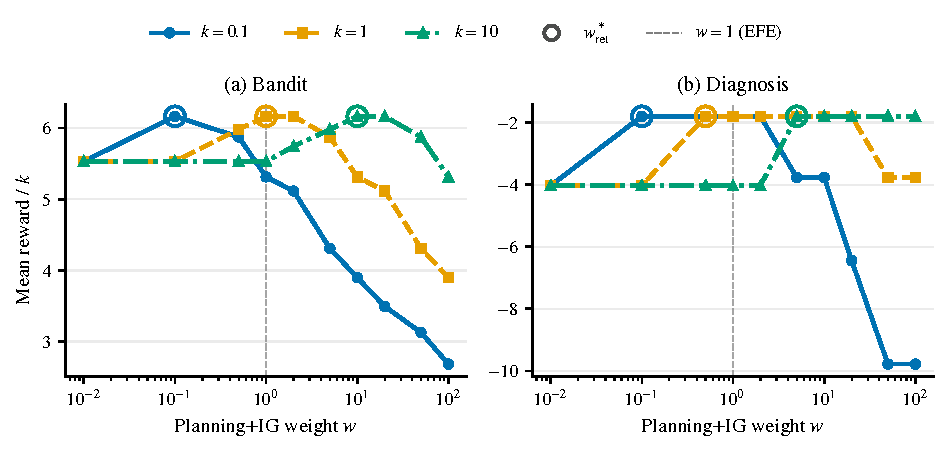
\includegraphics[width=0.78\linewidth]{figures/fig_reward_scaling.pdf}
\caption{Reward rescaling. Mean reward vs.\ Planning+IG weight $w$ under global scale factors $k$. Stars mark $w^*_{\mathrm{ret}}$. The optimum shifts toward larger $w$ as $k$ grows, consistent with $w^*_{\mathrm{ret}}(k) \propto k$.}
\label{fig:reward_scaling}
\Description{Two panels of mean reward versus weight on a log axis, each with three curves for scale factors 0.1, 1, and 10 and a dashed vertical line at weight 1. In the left Bandit panel the blue k=0.1 curve stays flat near 0 with a star at weight 0.1, the orange k=1 curve stays flat near 5 to 6 with a star at weight 1, and the green k=10 curve is flat near 55 before rising to a starred peak near 62 at weight 10, then falling back to about 53 at weight 100. In the right Diagnosis panel the blue k=0.1 curve stays flat near 0 with a star at weight 0.1, the orange k=1 curve stays flat near minus 2 to minus 4 with a star at weight 0.5, and the green k=10 curve is flat near minus 40 until weight 2, then jumps sharply to a starred plateau near minus 18 at weight 5 and stays there through weight 100.}
\end{figure}

\begin{table}[htbp]
\centering
\caption{Reward-optimal Planning+IG weight under reward scale $k$. The direction of covariance is as predicted (larger scales favor larger weights). On Bandit the ratio $w^*_{\mathrm{ret}}/k$ is exactly constant across the three tested scales under the fixed pipeline. On Diagnosis it varies twofold (flat high-$w$ plateaus mean several grid weights tie for $w^*_{\mathrm{ret}}$, and ties are broken toward the smallest weight reaching the maximum), so the table is qualitative evidence of covariance on Diagnosis and a tight quantitative match on Bandit, not a precise stability estimate on this finite grid.}
\label{tab:reward_scaling}
\begin{small}
\begin{tabular}{lccc}
\toprule
Environment & $k$ & $w^*_{\mathrm{ret}}$ & $w^*_{\mathrm{ret}}/k$ \\
\midrule
Diagnosis & $0.1$ & $0.1$ & $1.0$ \\
Diagnosis & $1.0$ & $0.5$ & $0.5$ \\
Diagnosis & $10.0$ & $5.0$ & $0.5$ \\
Bandit & $0.1$ & $0.1$ & $1.0$ \\
Bandit & $1.0$ & $1.0$ & $1.0$ \\
Bandit & $10.0$ & $10.0$ & $1.0$ \\
\bottomrule
\end{tabular}
\end{small}
\end{table}

\section{POMCP baseline comparison}
\label{app:pomcp}

We compare against POMCP \citep{silver2010}, a standard online POMDP solver that handles exploration through Monte Carlo tree search with UCB1 action selection. This addresses whether EFE's explicit information gain valuation provides benefit over the implicit exploration in POMCP's tree search. Our implementation adapts the algorithm to the observe-then-commit action structure, and three fidelity gaps against Silver and Veness must be stated before the numbers. Rollouts initialize from the agent's root belief regardless of tree depth, ignoring the observations accumulated along the tree path. The depth-cap leaf returns the best commit reward for the sampled state, a clairvoyant quantity. And rollouts credit the belief-expected commit reward rather than the sampled-state reward. The clairvoyant leaf and the belief-expected commit credit are favourable or neutral to POMCP on these small instances. The root-belief rollout cuts the other way, since it denies observation branches credit for the in-tree observations that produced them, so the net direction of these simplifications is mixed rather than uniformly favourable. None is present in the RockSample POMCP of Appendix~\ref{app:rocksample}, whose own departures from the published algorithm, all keyed to fully observable quantities, are stated there. Crucially, our POMCP rollout policy is semi-informed. Observation actions are selected uniformly at random, but the rollout terminates (stochastically, with 30\% probability per step) with a belief-optimal commit, i.e., the commit action maximizing expected reward under the Bayesian-updated rollout belief. This is strictly stronger than a fully random rollout, which would also randomize over commit actions. Each of the five outer seeds initializes both the environment stream and the planner's internal random stream (particle sampling and rollouts) from that seed, so the reported variability reflects genuine run-to-run differences rather than a fixed planner seed collapsing one axis of variation. Directed observation selection appears to be what separates EFE from POMCP here, though with the configuration caveats above we cannot fully separate it from solver configuration. EFE chooses which test to run based on information gain, while POMCP samples tests uniformly. We sweep POMCP simulation budgets across $\{500, 1000, 2000, 5000\}$ and report wall-clock timings for a simulation-budget scaling analysis. The comparison is simulation-matched, not compute-matched, the same distinction drawn for the MCTS-EFE comparison above. Tree-node action selection uses UCB1 with exploration constant $10.0$ (\texttt{rho\_aif/agents/pomcp.py}), fixed across all environments. This was not tuned per environment, and because reward scales differ across our benchmarks (Section~\ref{sec:experiments}), the same exploration constant implies a different effective exploration--exploitation balance on each one, a caveat symmetric to the reward-scale sensitivity we report for $w$ (Appendix~\ref{app:reward_scaling}). Tree and rollout depth are capped at the reporting agent's planning horizon plus three steps (\texttt{experiments/run\_pomcp.py}).

\begin{table}[htbp]
\centering
\caption{POMCP comparison config (5{,}000 total episodes across 5 per-run seeds $\{42,123,456,789,1024\}$ for Tiger/Diagnosis/Bandit and 1{,}000 for Tileworld, matching the main-table protocol on those three environments, and EFE/Planning here are re-run inside the POMCP harness rather than sourced from Table~\ref{tab:main}, which they reproduce exactly). POMCP uses 1{,}000 simulations per decision. Reward is mean $\pm$ seed-level SE. Bold marks EFE and any agent bit-identical to it, the convention of Table~\ref{tab:main}, so it flags EFE's row rather than a per-column best. On Tileworld $6{\times}6$ Planning is nominally ahead of EFE on both displayed metrics ($73.6\%$ against $71.9\%$, $-21.41$ against $-21.62$), and on Bandit POMCP(1000) leads on success ($87.7\%$ against $86.9\%$), both within seed-level sampling error.}
\label{tab:pomcp}
%% Numbers in this table are produced by experiments/run_pomcp.py
\begin{small}
\begin{tabular}{llccc}
\toprule
Environment & Agent & Obs. & Success & Reward \\
\midrule
\multirow{3}{*}{Tiger} & \textbf{Planning} & $\mathbf{4.20}$ & $\mathbf{99.4\%}$ & $\mathbf{+5.19 \pm 0.21}$ \\
& POMCP (1000) & $1.80$ & 89.4\% & $-3.48 \pm 0.28$ \\
& \textbf{EFE} & $\mathbf{4.20}$ & $\mathbf{99.4\%}$ & $\mathbf{+5.19 \pm 0.21}$ \\
\midrule
\multirow{3}{*}{Diagnosis} & Planning & $5.86$ & 88.8\% & $-2.57 \pm 0.20$ \\
& POMCP (1000) & $3.96$ & 74.1\% & $-9.49 \pm 0.22$ \\
& \textbf{EFE} & $\mathbf{9.66}$ & $\mathbf{97.2\%}$ & $\mathbf{-1.37 \pm 0.18}$ \\
\midrule
\multirow{3}{*}{Bandit} & Planning & $3.29$ & 71.0\% & $+5.75 \pm 0.08$ \\
& POMCP (1000) & $7.20$ & 87.7\% & $+5.29 \pm 0.04$ \\
& \textbf{EFE} & $\mathbf{5.11}$ & $\mathbf{86.9\%}$ & $\mathbf{+6.27 \pm 0.04}$ \\
\midrule
\multirow{3}{*}{\shortstack[l]{Tileworld\\[-1pt]{\scriptsize $6{\times}6$}}} & Planning & $15.57$ & 73.6\% & $-21.41 \pm 0.64$ \\
& POMCP (1000) & $1.35$ & 5.6\% & $-47.99 \pm 0.72$ \\
& \textbf{EFE} & $\mathbf{14.76}$ & $\mathbf{71.9\%}$ & $\mathbf{-21.62 \pm 0.87}$ \\
\bottomrule
\end{tabular}
\end{small}
\end{table}

\paragraph{Key findings.} Table~\ref{tab:pomcp} shows POMCP underperforming both EFE and Planning on reward on every environment, and on success rate everywhere except Bandit. On Tiger, POMCP commits prematurely (1.80 observations vs.\ 4.20 for EFE), yielding 89.4\% success against EFE's 99.4\% (here numerically identical to Planning, per the exact tie documented in Section~\ref{sec:results}). On Diagnosis, the gap is dramatic. POMCP achieves only 74.1\% success ($-9.49$ reward) while EFE reaches 97.2\% ($-1.37$ reward). POMCP's semi-informed rollout policy selects observation actions uniformly at random and so cannot evaluate which of the $K{=}2$ diagnostic tests to run. It treats all observation actions equally, whereas EFE's information gain term directly values differential informativeness. On Bandit, POMCP's Monte Carlo exploration achieves a slightly higher success rate than EFE ($87.7 \pm 0.5\%$ vs.\ $86.9 \pm 0.3\%$ seed-level SE, $+0.8$ pp) but at real reward cost ($+5.29 \pm 0.04$ vs.\ EFE's $+6.27 \pm 0.04$), buying that success with 7.20 inspections against EFE's 5.11. On success the two are close. EFE is ahead on reward. On Tileworld ($6{\times}6$, $|S|{=}36$), POMCP collapses to 5.6\% success, as the 36 commit actions and 6 scan actions create a branching factor that overwhelms 1{,}000 simulations.

\paragraph{Simulation-budget scaling.} Increasing POMCP's simulation budget to 5{,}000 does not qualitatively change the picture. On Diagnosis, POMCP(5000) reaches $75.5 \pm 0.6\%$ success (seed-level SE), still far short of EFE's $97.2 \pm 0.3\%$, while taking substantially more wall-clock time per episode (311.9 ms/ep vs.\ EFE's closed-form computation). On Tiger, POMCP(5000) reaches $90.3 \pm 0.3\%$ but at roughly 5$\times$ the compute of the 1{,}000-simulation budget. On Bandit the sweep is not monotone in the middle. POMCP(2000) reaches $90.8 \pm 0.3\%$ success at $+5.90 \pm 0.05$ reward, ahead of POMCP(1000) on both metrics and nominally above Planning's $+5.75$. POMCP(5000) then reaches $97.2 \pm 0.2\%$ success (clearly ahead of EFE) but its reward falls to $+5.18 \pm 0.04$ and its wall-clock cost balloons to roughly 0.93 s/episode, a $\sim$6.9$\times$ slowdown versus the 1{,}000-simulation budget. The 2{,}000-to-5{,}000 step is the clearest case in our results of buying success-rate with both compute and return. These results indicate that EFE's advantage is not merely a compute-budget artifact but reflects the benefit of closed-form information gain valuation over Monte Carlo exploration as configured here, with this rollout policy and a single untuned exploration constant, particularly on multi-observation-action environments where the agent must choose which information to gather. A stronger POMCP configuration (tuned exploration constants per reward scale, informed rollouts, or a reference implementation) could narrow the gap, and we do not claim the comparison bounds what a best-practice POMCP can achieve.

\paragraph{MCTS-EFE.} To disentangle EFE's information valuation from the planning mechanism, we implement MCTS-EFE. MCTS with EFE as the leaf heuristic rather than random rollouts, using UCB1 tree selection with max-backup value propagation and exact per-node information gain as the observe-action reward, so the tree optimizes the same objective as exact EFE rather than a proxy. On Tiger at $H{=}10$, MCTS-EFE with 500 simulations achieves 97.7\% success ($23$--$28$ ms per episode, \texttt{results\_mcts\_efe.csv}), compared to POMCP's 88.8\% at the same simulation count ($15$--$19$ ms per episode, simulation-matched, not compute-matched) and exact EFE's 99.9\% at $H{=}6$ ($103$ ms per episode, both from the MCTS battery's own 200-episodes-per-seed protocol rather than Table~\ref{tab:main}'s battery). In this configuration, EFE provides a stronger leaf evaluation function. The same MCTS framework with EFE leaf evaluation substantially outperforms semi-informed rollouts. We additionally ran a compute-matched check on this machine (\url{experiments/run_pomcp_compute_matched.py}), instrumented with seed-level statistics throughout. Timing MCTS-EFE(500) end to end for the full protocol (5 seeds $\times$ 200 episodes) gives 24.97s ($97.7\% \pm 0.5$pp success, seed-level SE). Calibrating POMCP's wall-clock cost at 200/500/1{,}000 simulations on the same protocol and machine and solving for the simulation budget matching 24.97s gives 699 simulations, roughly 40\% more than the simulation-matched comparison. POMCP(699) reaches $89.0\% \pm 0.8$pp success ($-3.82 \pm 0.81$ reward, $24.99$s), and a seed-level Welch test against the simulation-matched POMCP(500) ($88.8\% \pm 0.2$pp success, $-4.03 \pm 0.21$ reward, $19.08$s) confirms the two are not significantly different (success $p{=}0.81$, reward $p{=}0.81$). Giving POMCP the same wall-clock budget as MCTS-EFE rather than the same simulation count does not close the gap, and this is a direct test result rather than a bare assertion. Both POMCP configurations remain significantly behind MCTS-EFE on both metrics (seed-level Welch $p<0.0002$ in every comparison). On Tiger, MCTS-EFE's success and observation count are insensitive to both horizon (6, 8, 10) and simulation budget (200, 500, 1{,}000) in this range, saturating at 97.7\% success and 3.735 observations throughout. This reflects Tiger's small reachable-belief set, which the tree already covers well within 200 simulations, rather than the horizon or budget parameters having no effect in general.

\section{Budgeted $\rho$-POMDP supplementary details}
\label{app:budget_supp}

\subsection{SARSOP build and export details}
\label{app:sarsop_build}

Section~\ref{sec:sarsop}'s reference solver is the original APPL C++ toolkit (\texttt{pomdpsol}), built from source by \url{tools/build_sarsop.sh} with four documented patches required for a modern clang toolchain on Apple Silicon. Dropping unsupported \texttt{-msse2} and \texttt{-mfpmath=sse} flags, replacing raw-pointer \texttt{SparseCol} iterators (modern libc++ cannot construct \texttt{std::vector::const\_iterator} from a raw pointer), converting chained comparison assertions to conjunctions, and suppressing implicit-function-declaration errors in the legacy Cassandra parser. The resulting binary is not committed. The patch script is. \url{experiments/run_sarsop_baseline.py} exports any discrete observe-then-commit benchmark generically from the same hidden-state, action-layout, and observation-model definitions the agents already use (an absorbing done state, discount $\gamma{=}0.999$), solves to precision $10^{-3}$, parses the resulting alpha-vector policy from its XML output, and evaluates it through the same episode runner used for every other agent so that mechanics and metrics are shared exactly. Four unit tests (\url{tests/test_sarsop_export.py}) cover the exporter, the policy parser, and the alpha-vector argmax agent without requiring the compiled binary, so the export pipeline is checked even in environments where the solver is unavailable.

\subsection{Distractor-diagnosis environment: factorization guarantee}
\label{app:distractor}

Section~\ref{sec:distractor}'s \texttt{DistractorDiagnosisEnv} joint state space is the product of a $4$-way condition and a binary nuisance factor. Every observation model in the environment (condition tests, the distractor test, and the terminal commit reward) is constructed to depend on exactly one of the two factors, so for a belief that itself factors as a product of independent condition and nuisance marginals, observing the distractor test updates the nuisance marginal and leaves the condition marginal exactly unchanged, and symmetrically for condition tests and the nuisance marginal. This is verified by $13$ unit tests (\url{tests/test_distractor_diagnosis.py}), including a direct check that the condition marginal is unchanged before and after a distractor observation (up to floating-point tolerance) when the prior belief is factored, which makes their KL divergence exactly zero, and a symmetric check for condition tests against the nuisance marginal. The guarantee is stated for factored beliefs specifically. A belief with residual condition--nuisance correlation (which does not arise under this environment's independent generative process, but could under model misspecification) is outside the scope of the proof.

\subsection{The $w^*$ atlas}
\label{app:w_atlas}

Table~\ref{tab:w-atlas} aggregates the usage-curve range, implicit EFE budget $B_{\mathrm{EFE}} = U(w{=}1)$, and two canonical-budget crossing brackets (Definition~\ref{def:pi3}) for the eight benchmark instances whose usage curves were swept, generated by \url{experiments/run_w_atlas.py} from the saved usage-curve CSVs of Sections~\ref{sec:results} and~\ref{sec:budget_experiments}. Brackets are set-valued by construction. The table implies no closed-form relationship between $B_{\mathrm{EFE}}$ and environment parameters such as reward scale, state count, or horizon, and none should be inferred from it.

% Table auto-generated by experiments/run_w_atlas.py from
% results/results_w_atlas.csv -- see that script to regenerate.
% Auto-generated by experiments/run_w_atlas.py -- do not edit by hand.
\begin{table}[t]
\centering
\caption{Atlas of operational sensing budgets across benchmark instances:
 usage range of the Planning+IG family, implicit EFE budget
 $B_{\mathrm{EFE}} = U(w{=}1)$ (mean $\pm$ SE over seeds), and crossing
 brackets $w^*(B)$ at two canonical budgets per instance. Brackets are
 set-valued (Definition PI-3); no closed-form meta-model is implied.}
\label{tab:w-atlas}
\small
\begin{tabular}{lcccc}
\toprule
Instance & $[U_{\min}, U_{\max}]$ & $B_{\mathrm{EFE}}$ & $B_1$: $w^*$ bracket & $B_2$: $w^*$ bracket \\
\midrule
Bandit & $[3.06, 12.20]$ & $5.03 \pm 0.17$ & 4.4: $(0.0611, 0.139]$ & 10.8: $(19.3, 43.9]$ \\
Diagnosis & $[5.72, 13.57]$ & $9.68 \pm 0.15$ & 6.9: $(0.139, 0.316]$ & 12.4: $(19.3, 43.9]$ \\
Inspection-N16 & $[22.42, 46.04]$ & $33.46 \pm 0.19$ & 26.0: $(0.316, 1.33]$ & 42.5: $(5.62, 23.7]$ \\
Inspection-N8 & $[12.65, 30.89]$ & $18.24 \pm 0.19$ & 15.4: $(0.316, 2.15]$ & 28.2: $(14.7, 100]$ \\
RS{[}5,3{]} & $[3.81, 9.10]$ & $4.90 \pm 0.08$ & 4.6: $(0.316, 1.33]$ & 8.3: $(23.7, 100]$ \\
RS{[}7,4{]} & $[2.00, 14.73]$ & $5.49 \pm 0.14$ & 3.9: $(0.316, 2.15]$ & 12.8: $(14.7, 100]$ \\
Tiger & $[3.98, 5.62]$ & $4.21 \pm 0.07$ & -- & 5.4: $(19.3, 43.9]$ \\
Tileworld-6x6 & $[14.92, 33.70]$ & $14.83 \pm 0.22$ & 17.7: $(5.62, 23.7]$ & 30.9: $(23.7, 100]$ \\
\bottomrule
\end{tabular}
\end{table}


\section{JAIR reproducibility checklist}
\label{app:repro}

This appendix answers the JAIR reproducibility checklist \citep{gundersen2024jair} for the submission version of this article, as required for review. It is not part of the accepted version.

\subsection*{All articles}
\begin{enumerate}
\item All claims investigated in this work are clearly stated. \textbf{Yes.}
\item Clear explanations are given how the work reported substantiates the claims. \textbf{Yes.} Every proposition is accompanied by a proof or proof sketch (Section~\ref{sec:methodology}, Section~\ref{sec:budget}, Appendix~\ref{app:proof}), and every empirical claim is backed by a table or figure generated directly from committed result files.
\item Limitations or technical assumptions are stated clearly and explicitly. \textbf{Yes.} Section~\ref{sec:discussion} states scope limitations (observe-then-commit vs.\ factored observation coverage, the destructive-sensing boundary of Example~\ref{ex:destructive}, the single-reward-convention conditioning of every $w{=}1$ claim) and the conclusion restates them.
\item Conceptual outlines and/or pseudo-code descriptions of the AI methods introduced in this work are provided, and important implementation details are discussed. \textbf{Yes.} The recursive EFE agent (Equation~\ref{eq:efe_recursive}), the usage-curve procedure (Section~\ref{sec:budget}), and the online dual controller update are given in closed form in the main text, with build and export details for the SARSOP baseline in Appendix~\ref{app:sarsop_build}.
\item Motivation is provided for all design choices, including algorithms, implementation choices, parameters, data sets and experimental protocols beyond metrics. \textbf{Yes.} Section~\ref{sec:methodology} motivates the observe-then-commit restriction, and Section~\ref{sec:budget_positioning} positions every budgeted-formulation design choice against prior art.
\end{enumerate}

\subsection*{Articles containing theoretical contributions}
Does this paper make theoretical contributions? \textbf{Yes.}
\begin{enumerate}
\item All assumptions and restrictions are stated clearly and formally. \textbf{Partially.} Definition~\ref{def:factored} and the proposition preconditions state the structural assumptions. Proposition~\ref{prop:equivalence} states its four modeling assumptions ($\beta{=}1$ reward-to-preference identification, exact Bayesian conditioning, matched information units, deterministic $\arg\min$ selection) inside the proposition itself. The specific information base (bits in the implementation, nats in the canonical identification) is fixed in the surrounding text rather than in the proposition statement, and Proposition~\ref{prop:pi5} invokes the Robbins--Monro/Blum regularity conditions at the level of the cited theorems rather than restating them.
\item All novel claims are stated formally (e.g., in theorem statements). \textbf{Yes.} Propositions~\ref{prop:equivalence}, \ref{prop:nearopt}, \ref{prop:factored}, \ref{prop:pi1}, \ref{prop:pi2}, \ref{prop:pi5}, Definition~\ref{def:pi3}, and Corollary~\ref{cor:pi4}.
\item Proofs of all non-trivial claims are provided in sufficient detail to permit verification by readers with a reasonable degree of expertise. \textbf{Partially.} Full proof in Appendix~\ref{app:proof} for Proposition~\ref{prop:equivalence}. Proof sketches with the complete case analysis inline for the remaining propositions. Proposition~\ref{prop:pi5} appeals to the cited stochastic-approximation results rather than verifying their conditions line by line, and it covers the projected recursion, a variant of the implemented controller (Section~\ref{sec:budget}).
\item Complex formalism, such as definitions or proofs, is motivated and explained clearly. \textbf{Yes.}
\item The use of mathematical notation and formalism serves the purpose of enhancing clarity and precision; gratuitous use of mathematical formalism is avoided. \textbf{Yes.}
\item Appropriate citations are given for all non-trivial theoretical tools and techniques. \textbf{Yes.} Log scoring \citep{bernardo1979}, the Robbins--Monro recursion \citep{robbins1951} and its almost-sure convergence refinement \citep{blum1954}, and the sophisticated-inference Bellman-optimality result \citep{dacosta2020b} that the recursive agent is built on.
\end{enumerate}

\subsection*{Articles reporting on computational experiments}
Does this paper include computational experiments? \textbf{Yes.}
\begin{enumerate}
\item All source code required for conducting experiments is included in an online appendix or will be made publicly available upon publication of the paper. \textbf{Yes.} \url{https://github.com/PatrickAllenCooper/rho_aif}. PyPI distribution as \texttt{rho-aif} is planned but not yet published.
\item The source code comes with a license that allows free usage for reproducibility purposes. \textbf{Yes.} MIT License.
\item The source code comes with a license that allows free usage for research purposes in general. \textbf{Yes.} MIT License.
\item Raw, unaggregated data from all experiments is included in an online appendix or will be made publicly available upon publication of the paper. \textbf{Partially.} The repository commits, for every reported table and figure, the summary CSV it is built from, carrying per-agent means, and for the core-environment, Tileworld, Structural Inspection, transfer, IDS, scaling, discount, and navigation batteries also full protocol provenance (seed list, episodes per seed, git revision, generation timestamp), with the RockSample battery carrying the seed list and episodes per seed but not the git revision or generation timestamp. The offline-reference and atlas CSVs (SARSOP, CPOMDP, POMCP, MCTS-EFE, calibration, $w^*$ atlas) carry the summary statistics with their protocols stated in the corresponding table captions or accompanying prose instead. Per-episode traces are committed for the dual-control study. Episode-level frames for the remaining batteries are not committed as files, but the pipeline seeds every environment stream per episode, so they are regenerable exactly via the README's reproduction command map. The core-environment, Tileworld, RockSample, and Structural Inspection battery CSVs additionally carry both pooled and seed-level standard error columns directly (Structural Inspection's accuracy metric included), with companion \texttt{\_stats.csv} files reporting seed-level Welch $t$-tests, Cohen's $d$, and Holm--Bonferroni-corrected significance. The navigation-scaling and Diagnosis $N$-scaling batteries carry seed-level standard-error columns and companion \texttt{\_stats.csv} files as well. The IDS battery carries seed-level standard-error columns without a Welch companion, since the comparisons it supports are reported inline. Two batteries store point estimates only. These are the reward-rescaling sweep, whose qualitative claim (covariance of the tuned weight with the reward scale) does not rest on error bars, and the near-optimality horizon study, whose per-environment flags come from 50 episodes at a single seed and are reported as a descriptive boundary map rather than as estimates with uncertainty intervals.
\item The unaggregated data comes with a license that allows free usage for reproducibility purposes. \textbf{Yes.} Covered by the repository's MIT License.
\item The unaggregated data comes with a license that allows free usage for research purposes in general. \textbf{Yes.}
\item If an algorithm depends on randomness, then the method used for generating random numbers and for setting seeds is described in a way sufficient to allow replication of results. \textbf{Yes.} Main results use the canonical seed set $\{42, 123, 456, 789, 1024\}$ (documented in the repository README and the \texttt{rho\_aif.benchmark} module). Deviations are stated where they occur. The principal ones are three seeds for the reward-rescaling sweep, ten seeds for the multi-seed dual-control study of Section~\ref{sec:dual_multiseed}, ten seeds for RockSample RS[5,3] and RS[7,4] (500 episodes/seed), the canonical five seeds at 100 episodes/seed for RockSample RS[7,8] and RS[11,11], 500 episodes/seed for the Structural Inspection, discount, misspecification, IDS and transfer batteries, and 200 episodes/seed for the MCTS-EFE and Tileworld scaling sweeps. POMCP's internal random stream (particle sampling and rollouts) is seeded per-run from the same outer seed as the environment (Appendix~\ref{app:pomcp}), rather than from a fixed constant. Environment streams themselves are seeded per episode, with \texttt{env.reset} receiving the seed $10^4 s + i$ for outer seed $s$ and episode index $i$. Every environment stream is therefore seed-controlled end to end, the released pipeline's runs are bitwise reproducible, and every table and figure in this version was regenerated under it. Per-seed results are reported alongside aggregates wherever variation matters, including seed-level standard errors and $t$-tests for the three core environments (Table~\ref{tab:main}, Appendix~\ref{app:stats}).
\item The execution environment for experiments is described, including GPU/CPU makes and models, amount of memory, make and version of operating system, and names and versions of relevant software libraries and frameworks. \textbf{Partially.} All experiments are CPU-only, closed-form or Monte Carlo tree search computations with no GPU dependency and modest memory footprint (the largest benchmark, Structural Inspection, has $65{,}536$ states and runs in minutes on a laptop-class CPU). Exact make/model of the development machine is not pinned in the manuscript, and the dependency versions in \texttt{pyproject.toml} (Python $\geq 3.9$, NumPy, SciPy, Gymnasium, PyMDP, pandas, matplotlib, seaborn) are lower bounds rather than a fully pinned environment, so bit-exact reproduction may require matching the exact installed versions. The reported Monte Carlo quantities carry their own uncertainty estimates and are robust to version-level numerical differences.
\item The evaluation metrics used in experiments are clearly explained and their choice is explicitly motivated. \textbf{Yes.} Success rate, mean reward, mean observation count, and usage (sensing spend) are defined at first use and motivated by the observe-then-commit setting's cost structure (Section~\ref{sec:methodology}).
\item The number of algorithm runs used to compute each result is reported. \textbf{Yes.} Five seeds per condition unless stated otherwise (e.g., ten seeds for the multi-seed dual-control study of Section~\ref{sec:dual_multiseed}). Episode counts are reported per benchmark in the seeding item above and in every results table caption.
\item Reported results have not been ``cherry-picked'' by silently ignoring unsuccessful or unsatisfactory experiments. \textbf{Yes.} Section~\ref{sec:discussion} and the conclusion explicitly report where the proposed method does not help (Section~\ref{sec:distractor}'s distractor robustness result, Example~\ref{ex:destructive}'s destructive-sensing failure mode, and cases where tuned Planning+IG exceeds EFE on particular metrics).
\item Analysis of results goes beyond single-dimensional summaries of performance to include measures of variation, confidence, or other distributional information. \textbf{Yes.} Standard errors and confidence intervals are reported throughout Sections~\ref{sec:results} and~\ref{sec:budget_experiments} (e.g., the disjoint-CI comparison in Section~\ref{sec:dual_multiseed}, the mean $\pm$ SE usage-curve ranges of Appendix~\ref{app:w_atlas}).
\item All (hyper-)parameter settings for the algorithms/methods used in experiments have been reported, along with the rationale or method for determining them. \textbf{Yes.} Planning horizons and discount factors are reported per environment (Appendix~\ref{app:envs}) and the tuned Planning+IG weight search protocol is stated in Section~\ref{sec:methodology}, with discount-factor sensitivity swept explicitly in Appendix~\ref{app:discount}.
\item The number and range of (hyper-)parameter settings explored prior to conducting final experiments have been indicated, along with the effort spent on (hyper-)parameter optimisation. \textbf{Yes.} The Pareto sweep over $w$ (Section~\ref{sec:pareto}) reports the full grid searched, not only the selected operating point, and the horizon sweep of Appendix~\ref{app:nearopt_horizon} searches the horizon grid $H \in \{1,2,3\}$ and the weight grid $\{0.01, 0.5, 1, 2, 5, 50\}$, both stated in \url{experiments/run_nearopt_horizon.py}, from which its reward-optimal weight is selected.
\item Appropriately chosen statistical hypothesis tests are used to establish statistical significance in the presence of noise effects. \textbf{Yes.} Confidence intervals and seed-level $t$-tests (\texttt{tests/test\_stats\_seed.py}) are used rather than point-estimate comparisons alone. The SARSOP comparison of Section~\ref{sec:sarsop} is additionally backed by a predeclared-margin TOST equivalence test \citep{schuirmann1987}. The near-optimal CPOMDP reference of Section~\ref{sec:cpomdp} estimates the optimality gap directly via a Lagrangian-penalized SARSOP sweep, evaluated by simulation rather than a certified bound, in place of an informal consistency argument.
\end{enumerate}

\subsection*{Articles using data sets}
Does this work rely on one or more data sets? \textbf{No.} All environments (Tiger, Diagnosis, Bandit, Tileworld, RockSample, Structural Inspection, and the testbed variants) are simulators defined generatively in code (Appendix~\ref{app:envs}), not fixed empirical data sets. RockSample is a cost-modified variant of \citet{smith2004}, not the standard generator. Checks are charged, rock positions are fixed per instance in both ours and the original but use our own maps rather than the published ones, returns are undiscounted, exit is rewarded from any cell rather than only at the east edge, zero-range check accuracy is $0.95$ rather than perfect, and sampled rocks keep their hidden quality rather than turning bad (Section~\ref{sec:experiments} states all six, and notes that absolute returns are therefore not comparable to published RockSample numbers).

\subsection*{Explanations}
The execution-environment item above is answered Partially because this work's computational claims do not depend on hardware specifics. Every reported number is either a deterministic computation or a Monte Carlo estimate with reported variation, reproducible in distribution on any machine satisfying the stated minimum software versions. Each of the other Partially-marked items (theoretical assumptions and restrictions, proof completeness, and raw-data provenance) carries its own inline justification at that item.

\end{document}
